%%
%% Copyright 2007-2020 Elsevier Ltd
%%
%% This file is part of the 'Elsarticle Bundle'.
%% ---------------------------------------------
%%
%% It may be distributed under the conditions of the LaTeX Project Public
%% License, either version 1.2 of this license or (at your option) any
%% later version.  The latest version of this license is in
%%    http://www.latex-project.org/lppl.txt
%% and version 1.2 or later is part of all distributions of LaTeX
%% version 1999/12/01 or later.
%%
%% The list of all files belonging to the 'Elsarticle Bundle' is
%% given in the file `manifest.txt'.
%%

%% Template article for Elsevier's document class `elsarticle'
%% with numbered style bibliographic references
%% SP 2008/03/01
%%
%%
%%
%% $Id: elsarticle-template-num.tex 190 2020-11-23 11:12:32Z rishi $
%%
%%
\documentclass[preprint,10pt,times]{elsarticle}
\usepackage{ulem}
%% Use the option review to obtain double line spacing
%% \documentclass[authoryear,preprint,review,12pt]{elsarticle}

%% Use the options 1p,twocolumn; 3p; 3p,twocolumn; 5p; or 5p,twocolumn
%% for a journal layout:
%% \documentclass[final,1p,times]{elsarticle}
%% \documentclass[final,1p,times,twocolumn]{elsarticle}
%% \documentclass[final,3p,times]{elsarticle}
%% \documentclass[final,3p,times,twocolumn]{elsarticle}
%% \documentclass[final,5p,times]{elsarticle}
%% \documentclass[final,5p,times,twocolumn]{elsarticle}

%%%%%%%%%%%%%%%%%%%%%%%%%%%%%% User specified LaTeX commands.
\usepackage[scr=boondoxo]{mathalfa}
\DeclareFontEncoding{FML}{}{}
\DeclareFontSubstitution{FML}{fncmi}{m}{it}
\DeclareSymbolFont{fourierletters}{FML}{fncmi}{m}{it}
\SetSymbolFont{fourierletters}{normal}{FML}{fncmi}{m}{it}
\DeclareMathSymbol{\fP}{\mathalpha}{fourierletters}{`E}
\DeclareSymbolFont{Nperm}{OML}{cmss}{bx}{it}

\SetSymbolFont{Nperm}{bold}{OML}{cmss}{bx}{it}
\DeclareMathSymbol{\nw}{\mathalpha}{Nperm}{`w}
\newcommand{\unit}[1]{\ensuremath{\, \mathrm{#1}}}


\usepackage{amssymb,amsmath,yhmath,amsthm}
\newtheorem{theorem}{Theorem}[section]
\usepackage{lineno}
%\linenumbers
\usepackage{ccaption}
\usepackage{tabularx}
\numberwithin{equation}{section}
% \usepackage{showkeys}
\usepackage{todonotes}

\usepackage[T1]{fontenc}
% \usepackage{cite}
\usepackage{tikz}
\newcommand*\circled[1]{\tikz[baseline=(char.base)]{
\node[shape=circle,draw,inner sep=1pt] (char) {#1};}}


\usepackage{enumitem}
\usepackage{pifont}% http://ctan.org/pkg/pifont
\newcommand{\cmark}{\ding{51}}%
\newcommand{\xmark}{\ding{55}}%
\usepackage{epstopdf}
\usepackage{xr}
\usepackage{float}
\usepackage{hyperref}
\hypersetup{
colorlinks = true,
citecolor = blue,
linkcolor = blue
}

\newcommand{\tbp}[1]{\tilde{{\mathpzc{#1}}}}
\newcommand{\bp}[1]{{\mathpzc{#1}}}



% Proof reading
\PassOptionsToPackage{normalem}{ulem}
\usepackage{ulem}


% Special font for physical quantities
\newcommand{\forcemag}{f}
\newcommand{\physF}{\boldsymbol{\mathfrak{f}}} %
\newcommand{\physB}{\mathscr{b}} % Width of the thin film
\newcommand{\physE}{{\mathpzc{E}}}
\newcommand{\ndE}{E}
\newcommand{\ndL}{L}
\newcommand{\physI}{{\mathscr{I}}}
\newcommand{\ndI}{I}
\newcommand{\physkc}{\mathscr{k}_{\rm c}}
\newcommand{\ndkc}{k_{\rm c}}
\newcommand{\physh}{\mathscr{h}} %
\newcommand{\physe}{\hat{\mathbscr{e}}} %
\newcommand{\physf}{\hat{\boldsymbol{\mathfrak{f}}}}
\newcommand{\physm}{\mathscr{m}} %
\newcommand{\physu}{\mathbscr{u}}
\newcommand{\physw}{\mathscr{w}}
\newcommand{\rtple}[1]{\boldsymbol{#1}}
\newcommand{\n}{\mathfrak{n}} %

\newcommand{\physwc}{\bm{w}_c}
\newcommand{\physws}{\bm{w}_s}
\newcommand{\physwo}{\bm{w}_0}

\renewcommand{\u}[1]{\boldsymbol{#1}}
\newcommand{\chat}[1]{\skew{4}\hat{#1}}

\newcommand{\OriginRefEucldPtSpace}{O_{\mathrm{ R}}}
\newcommand{\MapManifoldToRefEucldPtSpace}{\kappa_{\mathrm{ R}}}
\renewcommand{\t}[1]{\tilde{#1}}
\renewcommand{\b}[1]{\mathbb{#1}}
\renewcommand{\c}[1]{\mathcal{#1}}
\newcommand{\lsc}[2][\mathscr{l}]{{}^{ #1 }\! #2}
\newcommand{\lscH}[1]{\lsc[H]{#1}}
\newcommand{\dsf}[1]{\Delta\boldsymbol{\sf #1}}
\newcommand{\tpsb}[1]{\left. #1 \right.^{\sf T}}
\newcommand{\tps}[1]{\left( #1 \right)^{\sf T}}
\newcommand{\usf}[1]{\u{\sf #1}}
\newcommand{\busf}[1]{\bar{\usf{ #1}}}
\newcommand{\tu}[1]{\tilde{\u{ #1}}}
\newcommand{\tusf}[1]{\tilde{\usf{ #1}}}
\newcommand{\btusf}[1]{\bar{\tusf{ #1}}}
\newcommand{\pr}[1]{\left( #1 \right)}
\newcommand{\encl}[1]{\left. #1 \right.}
\newcommand*{\subfigurewdith}{0.8\textwidth}
\newcommand{\D}[1]{D\hspace{-.1em}#1}
\newcommand{\Dr}{D\hspace{-.1em}\varrho}
\newcommand{\Drp}{\Dr^{+}}
\newcommand{\Drm}{\Dr^{-}}
\newcommand{\Dro}{\dot{\rho}}
\newcommand{\DDro}{\ddot{\rho}}
\newcommand{\Df}{\dot{f}}
\newcommand{\DDf}{\ddot{f}}
\newcommand{\Drop}{\Dro^{+}}
\newcommand{\Drom}{\Dro^{-}}
\newcommand{\Dl}{\dot{l}}
\newcommand{\Da}{\dot{a}}
\newcommand{\DDl}{\ddot{l}}
\newcommand{\DF}{\dot{F}}
\newcommand{\DDF}{\ddot{F}}
\newcommand{\Dlp}{\Dl^{+}}
\newcommand{\Dlm}{\Dl^{-}}
\newcommand{\Dam}{\Da^{-}}
\newcommand{\Deq}{\mathcal{D}^{\circ}}
\newcommand{\Dst}{\mathcal{D}^{\stable}}
\newcommand{\Dnt}{\mathcal{D}^{\odot}}
\newcommand{\Dunst}{\mathcal{D}^{\otimes}}
\newcommand{\conf}{\boldsymbol{\kappa}}
\newcommand{\confp}{\tilde{\boldsymbol{\kappa}}}
\newcommand{\gammaeq}{\gamma_{\text{sp-eq}}}





\newcommand{\hlc}[2][yellow]{ {\sethlcolor{#1} \hl{#2}} }
% \usepackage{wrapfig}

  \DeclareMathAlphabet{\mathvz}{OT1}{LinuxBiolinumT-OsF}{m}{sl}

  \DeclareMathAlphabet{\mathlib}{OT1}{LinuxLibertineT-OsF}{m}{it}
  \DeclareMathAlphabet{\mathbio}{OT1}{LinuxBiolinumT-OsF}{m}{it}
\DeclareMathAlphabet{\mathpzc}{OT1}{pzc}{m}{it}





\usepackage[prefix=sol]{xcolor-solarized}
\usepackage{booktabs}

% \usepackage{mathptmx}
\usepackage{pdflscape}
% \usepackage{threeparttable}
% \usepackage{tabto}

% \usepackage{sectsty}
%  \sectionfont{\fontsize{16}{16}\selectfont}

%CUSTOM COMMANDS
\newcommand{\norm}[1]{\ensuremath \lVert #1 \rVert}
\newcommand{\bs}[1]{\ensuremath{\mathbf{#1}}}
\newcommand{\pD}[2]{\frac{\partial #1}{\partial #2}}
\renewcommand{\D}[2]{\frac{\mathrm{d} #1}{\mathrm{d} #2}}
\newcommand{\dx}[1]{\,\mathrm{d} #1}
\newcommand{\ex}{{\bm{\hat{e}}}_1}
\newcommand{\ey}{{\bm{\hat{e}}}_2}
\newcommand{\ez}{{\bm{\hat{e}}}_3}
\newcommand{\ei}{{\bm{\hat{e}}}_i}
\newcommand{\ej}{{\bm{\hat{e}}}_j}
\newcommand{\er}{{\bm{\hat{e}}}_r}
\newcommand{\et}{{\bm{\hat{e}}}_\theta}
\newcommand{\ep}{{\bm{\hat{e}}}_\phi}
\newcommand{\TA}{\textit{Ta.\@}\xspace}
\newcommand{\EA}{\textit{Ea.\@}\xspace}
\newcommand{\subf}[1]{\pr{\textsf{#1}}}
\newcommand{\ra}[1]{\renewcommand{\arraystretch}{#1}}
\newcommand{\idp}{\mathsf{p}}


\newcommand{\notimplies}{%
  \mathrel{{\ooalign{\hidewidth$\not\phantom{=}$\hidewidth\cr$\implies$}}}}



%\usepackage[nomarkers,figuresonly]{endfloat}

\usepackage{algorithm,algorithmicx}
\usepackage{algpseudocode}
\usepackage[hang,flushmargin]{footmisc}
\DeclareMathOperator*{\argmin}{arg\,min} % Jan Hlavacek

\usepackage{xspace}
\newcommand\hmmax{0}
\newcommand\bmmax{0}
\usepackage{bm}
% \makeatother

% \usepackage{babel}
% \usepackage[style=numeric,backend=bibtex]{biblatex}

\journal{Journal of the Mechanical Behavior of Biomedical Materials}

\begin{document}

\begin{frontmatter}

%% Title, authors and addresses

%% use the tnoteref command within \title for footnotes;
%% use the tnotetext command for theassociated footnote;
%% use the fnref command within \author or \address for footnotes;
%% use the fntext command for theassociated footnote;
%% use the corref command within \author for corresponding author footnotes;
%% use the cortext command for theassociated footnote;
%% use the ead command for the email address,
%% and the form \ead[url] for the home page:
%% \title{Title\tnoteref{label1}}
%% \tnotetext[label1]{}
%% \author{Name\corref{cor1}\fnref{label2}}
%% \ead{email address}
%% \ead[url]{home page}
%% \fntext[label2]{}
%% \cortext[cor1]{}
%% \affiliation{organization={},
%%             addressline={},
%%             city={},
%%             postcode={},
%%             state={},
%%             country={}}
%% \fntext[label3]{}

\title{Sawtooth patterns in flexural force curves of structural biological
materials are not signatures of toughness enhancement: Part II}

%% use optional labels to link authors explicitly to addresses:
%% \author[label1,label2]{}
%% \affiliation[label1]{organization={},
%%             addressline={},
%%             city={},
%%             postcode={},
%%             state={},
%%             country={}}
%%
%% \affiliation[label2]{organization={},
%%             addressline={},
%%             city={},
%%             postcode={},
%%             state={},
%%             country={}}

\author{Wenqiang Fang}
\author{Sayaka Kochiyama}
\author{Haneesh Kesari\corref{cor1}}
\cortext[cor1]{Corresponding author}
\ead{haneesh\_kesari@brown.edu}

\address{Brown University, School of Engineering, 184 Hope Street, Providence, RI, USA}

\begin{abstract}
Stiff biological materials (SBMs), such as nacre and bone, are composites
that display remarkable toughness enhancements over their primary
constituents, which are brittle minerals. These enhancements are thought
to be a consequence of different mechanisms made possible by the SBMs'
internal lamellar architecture. One such mechanism is the Cook-Gordon
(crack-arrest-and-reinitiation) mechanism, whose operation manifests
in flexural tests as a sawtooth pattern in the force-displacement
curves. The curves from flexural tests carried out on marine sponge
spicules, which also possess a lamellar architecture, also display
a sawtooth-pattern, suggesting the presence of the Cook-Gordon mechanism.
Intriguingly, the spicules were recently found not to display any
significant toughness enhancement. To resolve this apparent contradiction,
in the preceding paper~[Kochiyama S, Monn MA, Fang W, Kesari H (2021): \textit{J Mech Behav Biomed Mater} 104362], we put forward the hypothesis that
the sawtooth pattern was due to the spicules slipping at the tests'
supports. In this paper, we present a model for the spicule's flexural
tests in which we allow for the possibility for the specimen to slip
at the test's supports. We model contact between the specimen and
the test's supports using the Coulomb's friction law. By choosing experimentally
reasonable values for the friction coefficient, we were able to get
the model's predictions to match experimental measurements remarkably
well. Additionally, on incorporating the spicules' surface roughness
into the model, which we did by varying the friction coefficient along
the spicule's length, its predictions can also be made to match the
measured sawtooth patterns. We find that the sawtooth patterns in the
model are due to slip type instabilities, which further reinforces
the hypothesis put forward in our preceding paper.

\end{abstract}

%%Graphical abstract
% \begin{graphicalabstract}
% %\includegraphics{grabs}
% \end{graphicalabstract}

%%Research highlights
% \begin{highlights}
% \item Research highlight 1
% \item Research highlight 2
% \end{highlights}

\begin{keyword}
%% keywords here, in the form: keyword \sep keyword

%% PACS codes here, in the form: \PACS code \sep code

%% MSC codes here, in the form: \MSC code \sep code
%% or \MSC[2008] code \sep code (2000 is the default)
structure-property relationship \sep experimental mechanics \sep stick-slip phenomenon \sep architectured materials
\end{keyword}

\end{frontmatter}

%% \linenumbers

%% main text
\section{Introduction\label{sec:Introduction}}

Stiff biological materials (SBMs), such as nacre and bone, are natural
layered composites that are known for having remarkable fracture toughness
that can be orders of magnitude higher than that of the brittle ceramics
that dominates their composition~\cite{jackson1988mechanical,currey1977mechanical,sarikaya1994introduction,menig2000quasi,koester2008true,wegst2015bioinspired}.
The key to such enhancement in fracture toughness lies in their lamellar
architectures, which are the intricate arrangements of ceramic and
organic phases at the sub-micron scales (see Figure~\ref{fig:lamellar}$\subf{A}$\&$\subf{B}$).
One way in which the lamellar architecture contributes to the toughness
enhancement is by supporting the operation of the Cook-Gordon (crack-arrest-and-reinitiation)
mechanism)~\cite{cook1964mechanism}. In this mechanism, when a crack
initiates in and propagates through the ceramic phase, the organic
phase, which separates one region of the ceramic phase from another,
can effectively act as a \textquotedblleft trap\textquotedblright{}
and arrest the crack~\cite{ming1989crack,cook1964mechanism}. In
flexural tests, the operation of the Cook-Gordon mechanism reflects
as a drop in the measured force as the crack advances, and then as
the end of that force drop as the crack gets arrested~\cite{clegg1990simple}.
As such, when the Cook-Gordon mechanism operates in layered materials,
the measured force-displacement curve can have the appearance of a
sawtooth pattern (see Figure~\ref{fig:sawtooth}$\subf{B}$).

\begin{figure}
\begin{centering}
\includegraphics[width=1\textwidth]{../Figures_Submit/Lamellar_V3.pdf}
\par\end{centering}
\caption{\label{fig:lamellar} Lamellar architectures in biological materials.~$\subf{A}$
The shell of~\textit{Haliotis rufescens}---the red abalone (image
courtesy of John Varner).~$\subf{B}$ The nacre from~\textit{H. rufescens}
consists of aragonite tablets assembled in a brick-and-mortar manner,
where thin protein layers (not identifiable in the image) in-between
the tablets function as the mortar (modified with permission from~\cite{rabiei2012nacre}; copyright 2012 the Royal Society of Chemistry). Owing to such arrangement,
nacre demonstrates a 1000-fold increase in fracture toughness compared
to that of the mineral aragonite.~$\subf{C}$ The entire skeletal
structure of a marine sponge~\textit{Euplectella aspergillum} is
shown (modified from~\cite{monn2015new}; copyright 2015 National Academy of Sciences). The white arrow identifies
the spicules, which are around 50$~\mu$m in diameter and can be several
centimeters long. In some of our recent studies, we performed three-point
bending tests on these spicules~\cite{monn2017enhanced,monn2020lamellar}.~$\subf{D}$
A scanning electron microscope (SEM) image of a~\textit{E. aspergillum}
spicule's cross section shows lamellar architecture consisting of
a cylindrical silica core surrounded by concentric silica layers (modified
from~\cite{monn2015new}; copyright 2015 National Academy of Sciences). Each of these concentric silica layers
are separated from their adjacent layers or the silica
core  by a compliant organic layer whose thickness
is roughly in the 5--10 nm range (not identifiable in the SEM image)~\cite{weaver2007hierarchical}.}
\end{figure}

\begin{figure}
\centering{}
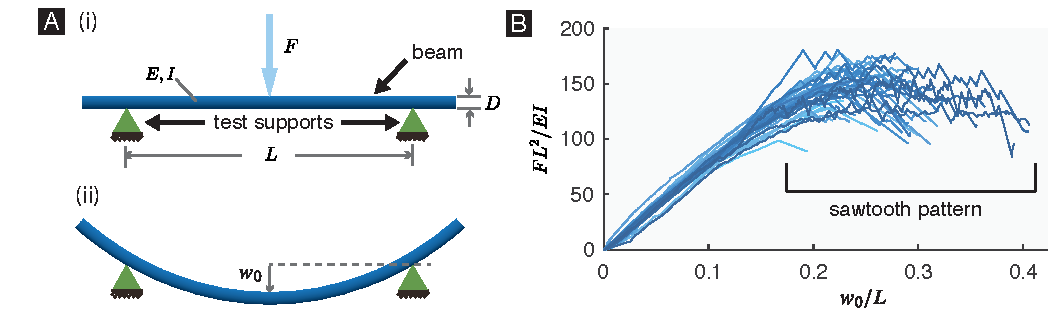
\includegraphics[width=1\textwidth]{../Figures_Submit/SawtoothPatterns_V4.pdf}
\caption{\label{fig:sawtooth}~$\subf{A}$$\subf{i}$ Typical schematic of
a three-point bending test in its reference configuration and~$\subf{ii}$
the deformed beam with midpoint displacement~$w_0$ under the action of some midpoint force~$F$. % hk done
The support span is~$\ndL$, and~$D$,~$\ndE$, and~$\ndI =\pi D^4/64$
are the diameter, Young's modulus, and the bending moment of inertia of
the beam, respectively. % hk done
$\subf{B}$ Thirty eight scaled force-displacement
curves from three-point bending
tests carried out on \textit{E. aspergillum} spicules and previously presented in~\cite{monn2017enhanced,Sayaka2021Sawtooth}. % hk done
The spicules respond linearly until a certain point, then, in most cases, start displaying the sawtooth pattern. % hk done
}
\end{figure}

\begin{figure}
\centering{}
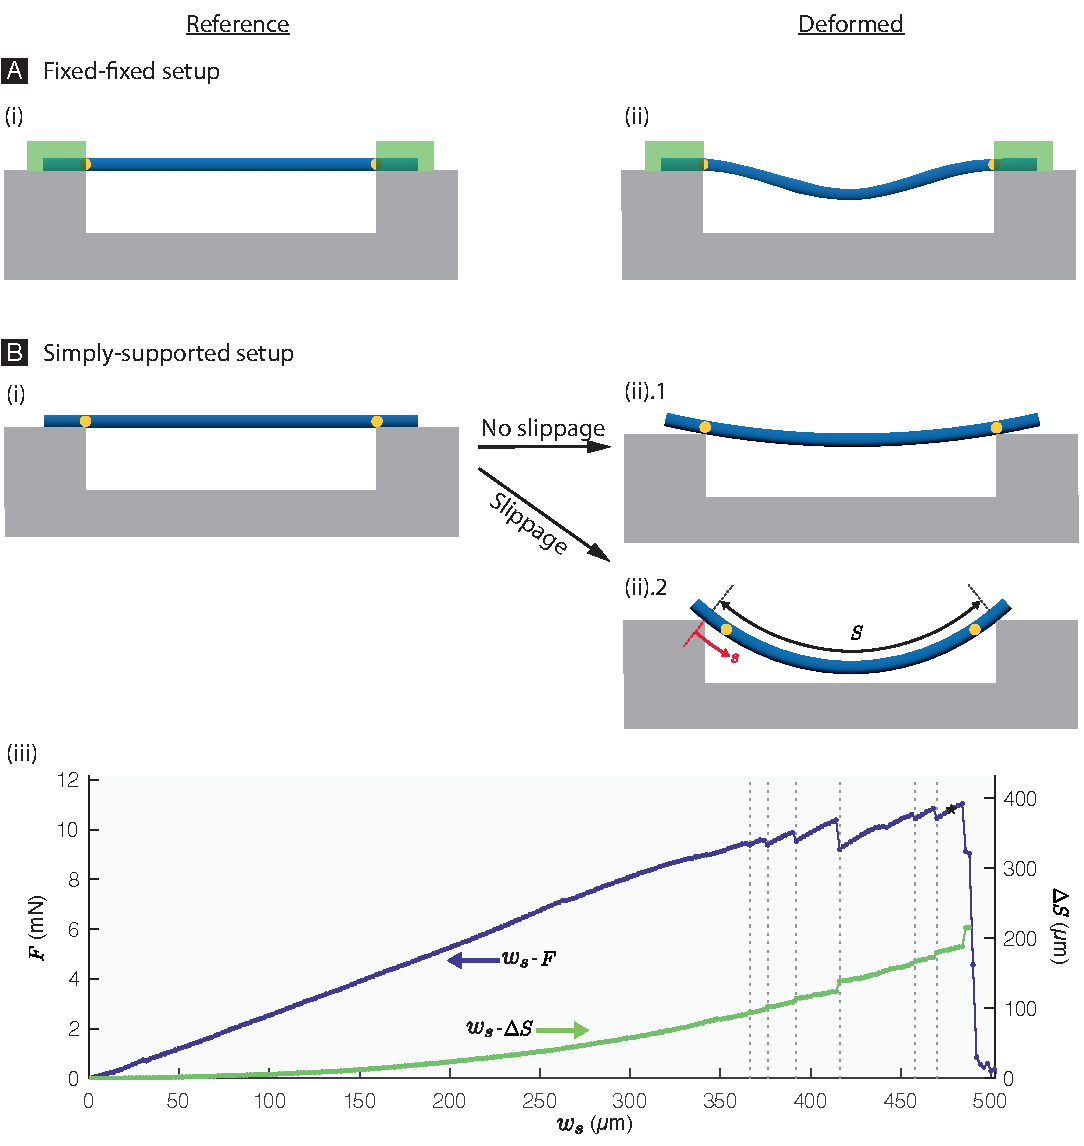
\includegraphics[width=1\textwidth]{../Figures_Submit/Slip_V8.pdf}
\caption{Fixed-fixed setup and spicule slippage in simply-supported
setup.
$\subf{A}$$\subf{i}$ shows the reference configuration of
a spicule set up for a flexural test in a fixed-fixed setup; the spicule
ends are glued onto the test's supports (adhesive shown in green). The yellow circles mark two spicule material particle that sit at
the test's supports in this configuration. % hk done
$\subf{A}$$\subf{ii}$ shows the spicule in its deformed configuration as it is being tested with its ends glued to the test's supports. The material particles that were at the test's supports in the reference configuration (yellow circles) are still at the test's supports. % hk done
$\subf{B}$$\subf{i}$ shows a spicule in its reference configuration in the simply-supported setup. % hk done
The yellow circles mark two spicule material particle that sit at
the test's supports in this configuration. % hk done
(Caption continued on next page)}
\label{fig:slip2}
\end{figure}


\begin{figure}
\centering
\contcaption{ (continued from previous page)
$\subf{B}$$\subf{ii}.1$ shows a deformed spicule configuration
in which the spicule has not undergone any slipping at the supports; the material particles that were at the test's supports in the reference configuration (yellow circles) are still at the test's supports in this configuration as well. % hk done
This is the assumption made in standard beam theories, such as the Euler-Bernoulli beam theory, when they are used to model three point bending tests. % hk done
~$\subf{B}$$\subf{ii}.2$
shows a deformed configuration of the spicule in which the spicule has undergone slippage at the test's supports. % hk done
The material particles denoted by the yellow circles are no longer at the test's supports,
but have slipped down into the trench. % hk done
The parameter~$S$ denotes the spicule's total length, which is the length of the section
of the spicule specimen lying between the test's supports. % hk done
~$\subf{B}$$\subf{iii}$ shows the measured force~$F$ (left axis) (for details
of what we mean by force,~$F$, see~$\S$\ref{sec:experiment})
and the change in the total length,~$\Delta S$ (right axis), from a  representative three point bending test carried out in the simply supported setup as a function of stage displacement,~$w_s$, in
blue and green, respectively. % hk done
The vertical dashed lines indicate the
instances at which the drops in the force take place. % hk done
As can be noted from the graphs, the
jumps in the spicule's total length take place at those very same instances (modified from~\cite{Sayaka2021Sawtooth}). % hk done
\label{fig:slip2}}
\end{figure}

\medskip{}


Monn et al. recently showed that the presence of lamellar architectures
by itself does not necessarily guarantee the operation of the Cook-Gordon
mechanism~\cite{monn2020lamellar}. They demonstrated this using
the fiber-like glass skeletal elements, called spicules (see Figure~\ref{fig:lamellar}$\subf{C}$),
of the marine sponge~\textit{Euplectella aspergillum} ($\EA$).
The~$\EA$ spicules also have a lamellar architecture that resembles
those in nacre and bone. The architecture consists of alternating
layers of glass and organic phase laid out in a concentric manner,
as shown in Figure~\ref{fig:lamellar}$\subf{D}$. Monn et al. performed
notched three-point bending tests on the spicules and directly measured
their fracture toughness in terms of the initiation fracture toughness
and the average crack growth resistance, and found that the fracture
toughness enhancement in them was negligible~\cite{monn2020lamellar}.
This implied that the Cook-Gordon mechanism either operated to a negligible
level or was absent in the spicules.

\medskip{}

However, the implication that the Cook-Gordon mechanism operates to
an insignificant level during the failure of~$\EA$ spicules in flexural
tests appears to contradict the observations made in Monn and Kesari~\cite{sarikaya2001biomimetic,levi1989remarkably,monn2017enhanced}.
To be specific, in~\cite{monn2017enhanced} Monn and Kesari carried
out three-point bending tests on~$\EA$ spicules. They observed sawtooth
patterns in the force-displacement curves from their tests, in which
the spicules were being loaded all the way until failure (see Figure~\ref{fig:sawtooth}).
As \sout{we }intimated previously, sawtooth-patterns in layered materials
are usually a signature of the operation of the Cook-Gordon mechanism~\cite{clegg1990simple}
. \sout{So if, as argued in Monn et al., the Cook-Gordon mechanism is indeed
irrelevant during the spicule's failure, then how does one explain
the sawtooth patterns observed in the force-displacements curves of
Monn and Kesari?}
\textcolor{red}{Therefore, if the Cook-Gordon mechanism is indeed
irrelevant during the spicule's failure as argued in Monn et al., there must be alternative explanations for the appearance of the sawtooth patterns observed in the force-displacements curves of Monn and Kesari.}

In Part I of the current paper~\cite{Sayaka2021Sawtooth}, we attempt
to resolve the apparent contradiction by hypothesizing that the sawtooth
patterns, at least in the case of~$\EA$ spicules, are solely the
consequence of the spicules slipping (see Figure~\hypersetup{linkcolor=red}\ref{fig:slip2}\hypersetup{linkcolor=blue}$\subf{B}$)
at the test's supports, rather than of the operation of the Cook-Gordon
mechanism. We summarize our arguments from Part I of this paper in
the following few paragraphs.

\medskip{}

In~\cite{Sayaka2021Sawtooth} we reported force-displacement measurements
from three-point bending tests that \sout{we}\textcolor{red}{were} carried out on~$\EA$ spicules
in the simply-supported (SS) setup (see Figure~\ref{fig:sawtooth}).
Micrographs of the spicules were taken\textit{ in-situ} via a microscope
during the tests. By conducting image analysis on those micrographs,
\sout{we}\textcolor{red}{it was} demonstrated that in the tests in which the force-displacement
curve displayed a sawtooth pattern, there were sudden jumps in the
total length of the spicule section lying between the test's supports.
This total length is shown marked as~$S$ in Figure~\hypersetup{linkcolor=red}\ref{fig:slip2}\hypersetup{linkcolor=blue}$\subf{B}$$\subf{ii}.2$.
The jumps appear, e.g., as the discontinuities in the green curve
shown in Figure~\hypersetup{linkcolor=red}\ref{fig:slip2}\hypersetup{linkcolor=blue}$\subf{B}$$\subf{iii}$.  \sout{We then
showed}\textcolor{red}{It was further shown} that the jumps and the force-drop events (which appear, e.g.,
as the discontinuities in the blue curve in Figure~\hypersetup{linkcolor=red}\ref{fig:slip2}\hypersetup{linkcolor=blue}$\subf{B}$$\subf{iii}$)
took place at the exact same time instances. These observations imply
one of the following three scenarios: (i) the force-drop events are
solely due to the layer-fracture events associated with the Cook-Gordon
mechanism, (ii) they are due to a combination of layer-fracture events
and slip-events, or (iii) they are entirely due to the slip-events.

To determine which of the three scenarios is likely true, \sout{we again
carried out} three-point bending tests \textcolor{red}{were carried out} on the spicules \textcolor{red}{again} \sout{but this time}
in the fixed-fixed (FF) setup (see Figure~\hypersetup{linkcolor=red}\ref{fig:slip2}\hypersetup{linkcolor=blue}$\subf{A}$).
In the FF setup, the spicule's ends are glued to the test's supports,
which prevents the occurrence of any slip-events at the test's supports.
None of the force-displacement curves from the FF tests displayed
a sawtooth pattern. \sout{This observation led us to conclude that it was
scenario (iii) that was true. In arriving at this conclusion, we,
however, implicitly assumed that the operation of the Cook-Gordon
mechanism would be unaffected regardless of whether or not the spicule
ends are free to slide and rotate. For that reason, we attempted to
gauge the likelihood of the different scenarios being true through
a different means.}\textcolor{red}{Although this observation points to scenario (iii) as being true, it is with the implicit assumption that the operation of the Cook-Gordon
mechanism would be unaffected regardless of whether or not the spicule
ends are free to slide and rotate. Since such an assumption is not explicitly validated, additional experiments were performed to gauge the likelihood of each of the three scenarios in an alternative manner. } \sout{We repeated the three-point bending tests on the
spicules in the SS setup. However, this time, instead of loading them
all the way until they failed completely, we only loaded them until
we observed a few force drops that are characteristic of the sawtooth-pattern.}\textcolor{red}{To be specific, the three-point bending tests were carried out on the spicules again in the SS setup, but the spicules were only loaded until a few force drops that are characteristic of the sawtooth-pattern were observed instead of until complete failure.}
\sout{We then unloaded the}\textcolor{red}{The} specimens \textcolor{red}{were then unloaded} until they regained their straight
shape and the force on them almost vanished. Finally, \sout{we loaded the
spicules again (re-loaded them) until we again observed a few force
drops.}\textcolor{red}{the spicules were loaded for the second time (re-loaded) until a few force drops were again observed.} If the sawtooth pattern observed during the loading phase was
due to the Cook-Gordon mechanism, then the spicule's stiffness (slope
of the initial linear portion of the force-displacement curve before
the appearance of the force drops) from the re-loading (second loading)
phase should be different from that in the loading (first loading)
phase. However, \sout{we found} the spicules' stiffnesses in the loading
and the re-loading phases \textcolor{red}{were found }to be almost the same. This observation
implies that the force-drops in the loading phases are not due to
the Cook-Gordon mechanism, which leads us to conclude that scenario (iii)
is the one that is true.

In this paper, with the goal of further investigating our hypothesis,
we develop and study a mechanics model for the spicule's SS bending
tests. A distinguishing feature of our model is that \sout{in it} the test
specimen is allowed to slide at the test's supports. In contrast,
in the standard Euler-Bernoulli (EB) model of the three point bending
test, the specimen is not allowed to slide at the test's supports.

\medskip{}

Considering the geometry in the SS experiments\textcolor{violet}{{}
}(e.g., see Figure~\ref{fig:sawtooth}), in our model\textcolor{red}{,} \sout{we take that}
the spicule's displacements\textcolor{red}{~are taken} to be two dimensional in nature. \sout{Considering
the spicules' high aspect ratios (length:diameter) of~$\approx 25$,
we model them as 1D continua. Since the spicules undergo large displacements
in the experiments, we use the Euler's elastica theory to model their
bending behavior. We ignore any stretching behavior along their axes.}
\textcolor{red}{The spicules are modeled as 1D continua considering their high aspect ratios (length:diameter) of~$\approx 25$, and their bending behavior is modeled using Euler's elastica theory since they undergo large displacements in the experiments. Any stretching behavior along their axes are ignored.}
The contact at the test's supports is modeled using the Coulomb friction
model. Scanning electron microscopy (SEM) revealed that the spicules'
surfaces could have both smooth and rough regions.
By roughness, we are referring to the different types of imperfections,
including debris, scrapes and outer layer damage, that \sout{we}\textcolor{red}{were} observed
on the spicules' surfaces (Figure~\ref{fig:SEM}). We incorporate
the spicules' surface roughness in our model by assuming that the
coefficient of friction between the spicule and the test's supports
varies depending on which particular spicule cross-section is in contact
with the supports. Specifically, in the model \sout{we assume}\textcolor{red}{it is assumed} that the coefficient
of friction varies along the spicule's length  as
\begin{equation}
\mu_{0}\left(1+A\cos\left(\frac{ 2 \pi s}{\lambda}-\phi\right)\right),\label{eq:muofS1}
\end{equation}
where~$s$ is the arc-length coordinate along the spicule's axis
(see Figure~\hypersetup{linkcolor=red}\ref{fig:slip2}\hypersetup{linkcolor=blue}$\subf{B}$$\subf{ii}.2$), and we refer
to the parameters~$\mu_0$,~$A$,~$\lambda$, and~$\phi$ as the
average value of coefficient of friction, the amplitude, the wavelength,
and the phase, respectively. In our problem, \sout{we take} the static and
kinetic coefficients of friction \textcolor{red}{are taken} to have the same value. In~$\S$\ref{subsec:Governing-equations-of},
we present the governing equations of our model. In~$\S$\ref{subsec:Equilibrium-force-displacement},
we semi-analytically solve the governing equations to derive what
we call our model's equilibrium force-displacement curve. \textcolor{red}{Each point on that curve corresponds to a static equilibrium configuration.}
Our model
predicts that any measured force-displacement point will lie on the
equilibrium curve. However, due to the finite stiffness of the loading
apparatus, not all the points on the equilibrium curve will be measured
in an experiment. Taking into account the stability of the equilibrium
points in~$\S$\textcolor{violet}{\ref{subsec:Force-displacement-curves-that}},
we provide an algorithm for numerically determining our model's prediction
for the force-displacement curve that will be measured in an SS experiment.

\begin{figure}
\begin{centering}
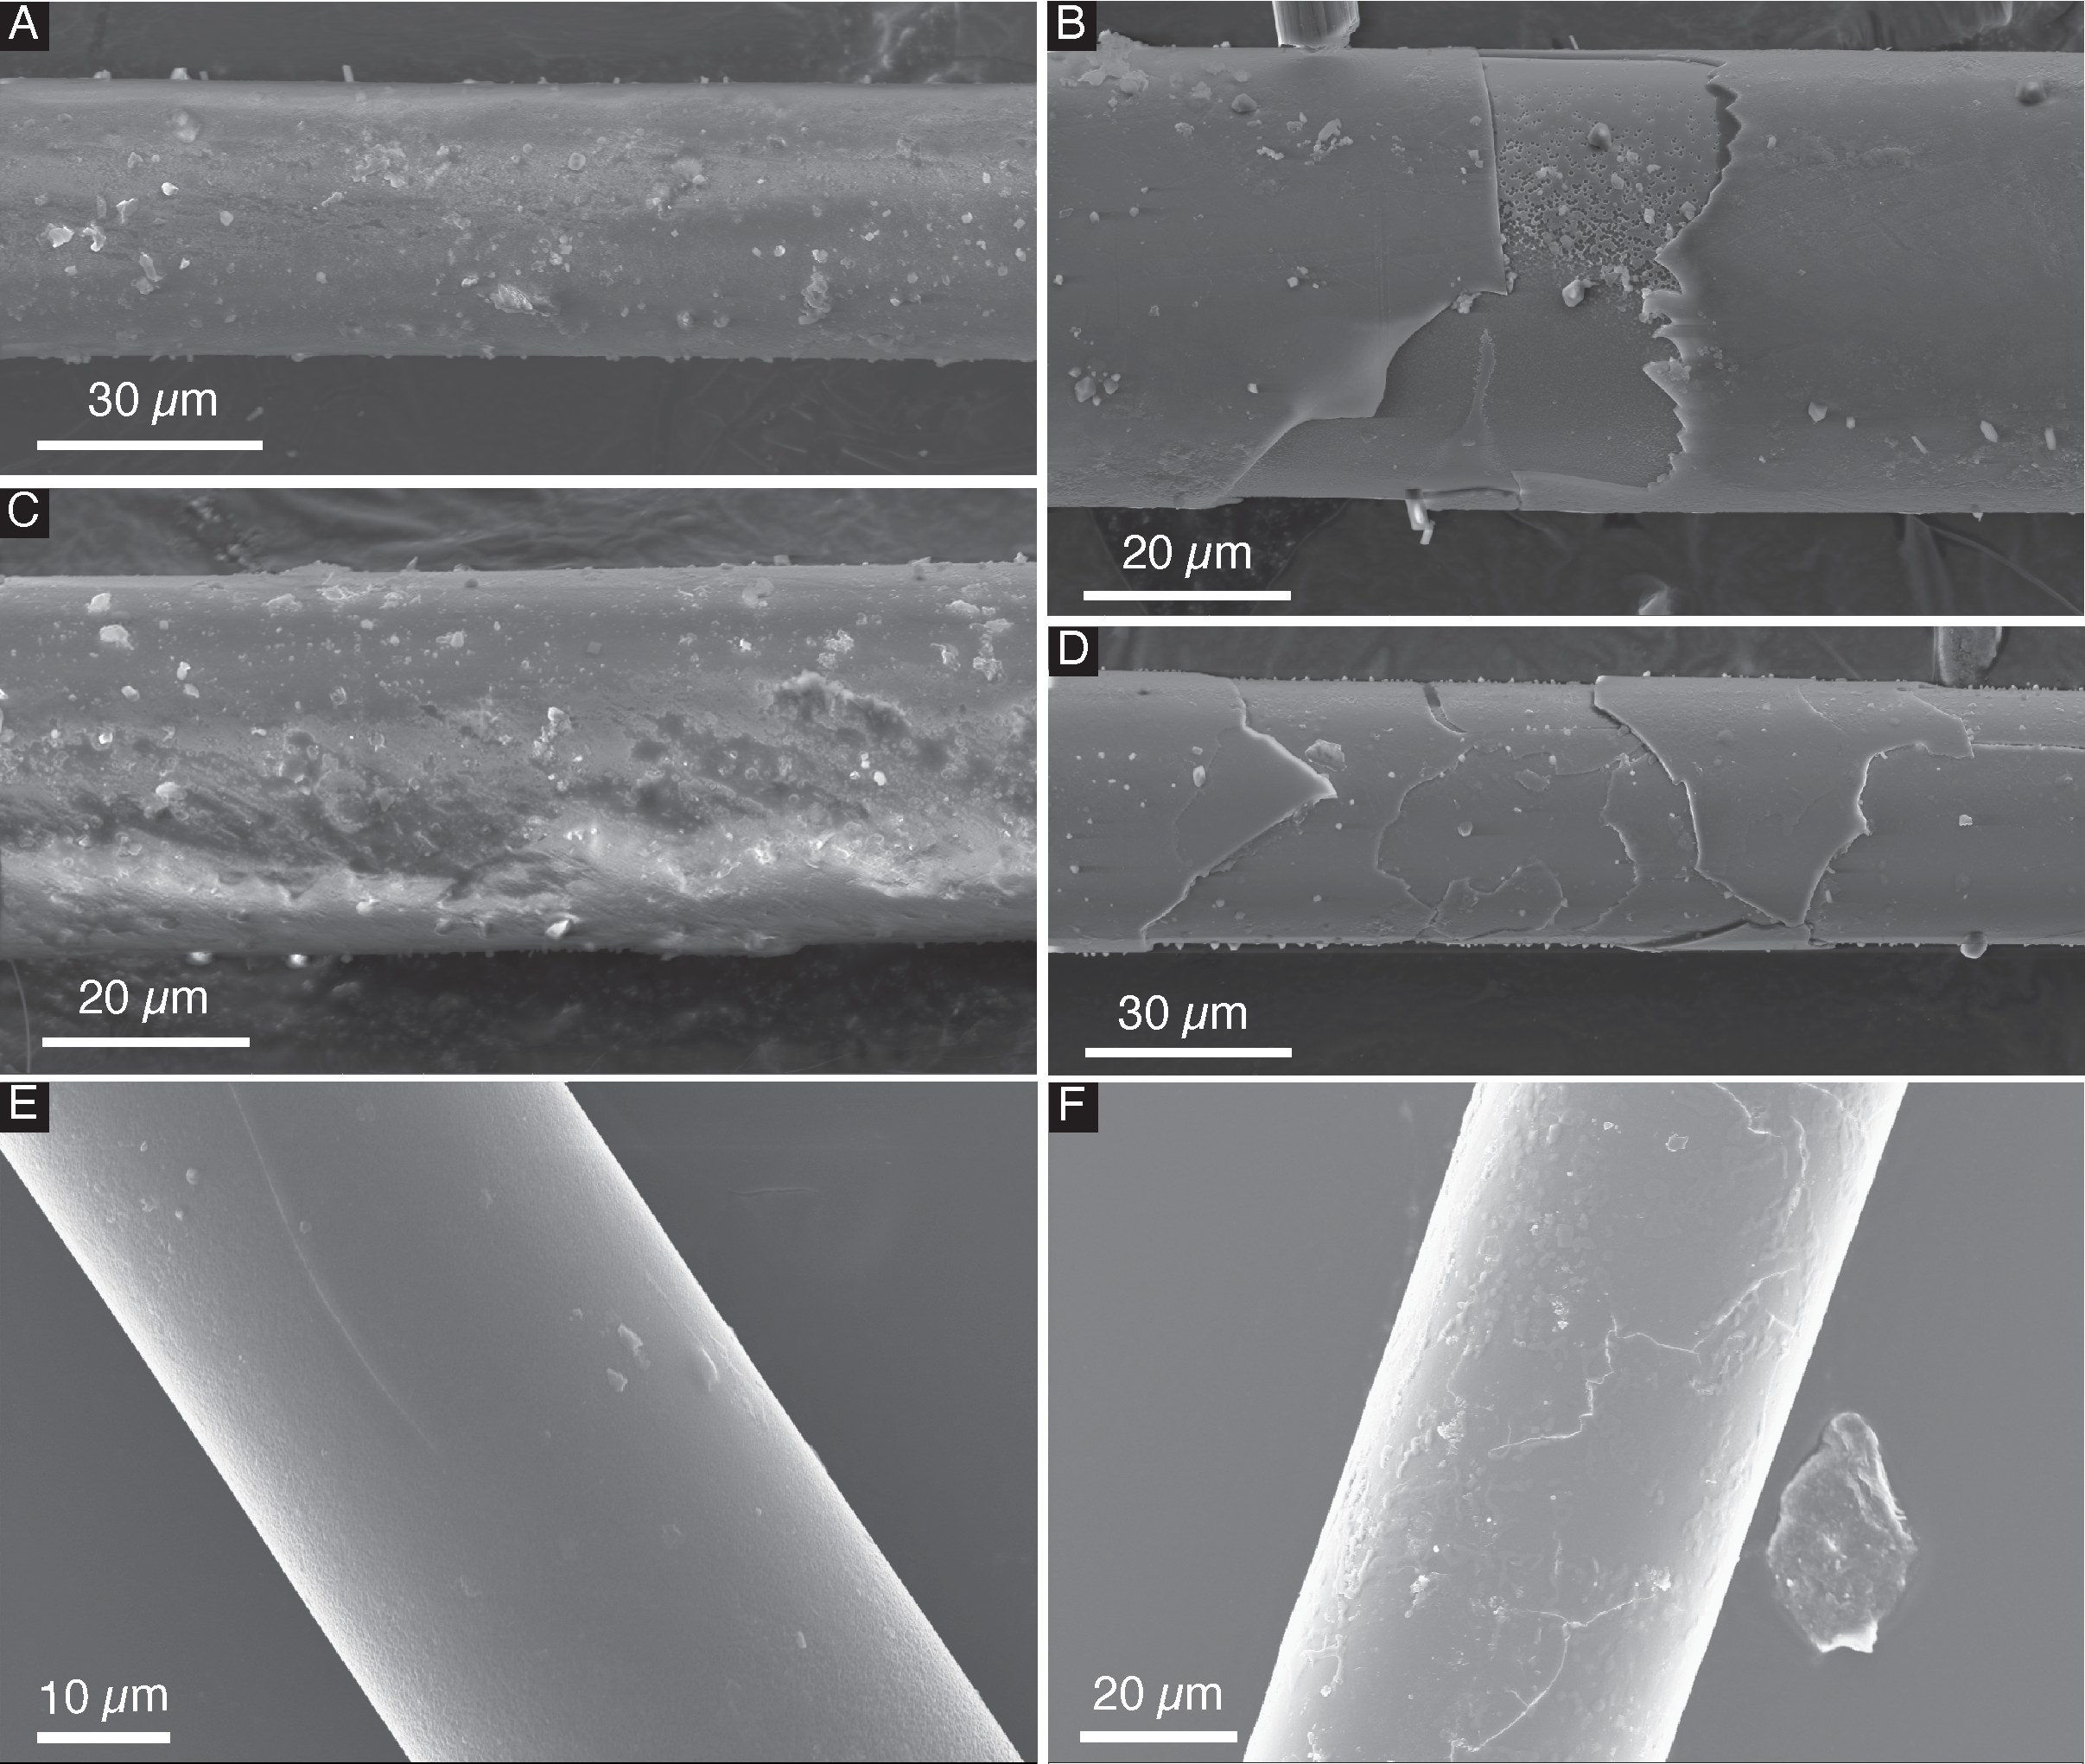
\includegraphics[width=1\textwidth]{../Figures_Submit/EA_SEM.pdf}
\par\end{centering}
\caption{
\label{fig:SEM}
Representative SEM images of a few
randomly selected~\textit{E. aspergillum} spicules that were taken after the spicules had been flexurally tested in a simply-supported setup. % hk done
Each spicule is identified by the label given to the
flexural test (see Tables S1--S2 of~\cite{Sayaka2021Sawtooth} for detailed
information pertaining to a given test) in which it was used. % hk done
$\subf{A}$ and~$\subf{B}$ are two
different images of the spicule from the test SS4. % hk done
$\subf{C}$--$\subf{F}$ are images of
the spicules from the tests  SS7,
SS24, SS32, and SS34, respectively. % hk done
The imaged region in each spicule was chosen randomly. % hk done
These images demonstrate how the spicules can have rough
surfaces, as shown in~$\subf{A}$--$\subf{D}$, or relatively smooth
surfaces, as shown in~$\subf{E}$--$\subf{F}$. % hk done
}
\end{figure}


In~$\S$\ref{sec:comparison}, we compare the force-displacement
curves predicted by our models with the ones that were experimentally
measured in~\cite{monn2017enhanced,Sayaka2021Sawtooth}. We find
that not only do the predicted force-displacement curves capture the
sawtooth pattern, \textcolor{red}{but} they \sout{in fact} can also be made to quantitatively
match the measured force-displacement remarkably well by appropriately
choosing the value of~$\mu_0$,~$A$,~$\lambda$, and~$\phi$\sout{
in our model}. The sawtooth pattern in our model is a direct consequence
of the slip events at the supports. \sout{We find that the values we chose
for~$\mu_0$, while trying to get our model's prediction to match
the experimental measurements,}\textcolor{red}{We find that the values of~$\mu_0$, which were chosen to match our model's prediction with the experimental measurements,} is quite consistent with the values
reported in literature for the coefficient of friction between glass
and steel (note that the contact in the spicule SS experiments is
between silica (spicule) and stainless steel (test's supports)).

Since the sawtooth pattern in our model is a direct consequence of
slip events, the good match between our model's predictions and the
experimental measurements supports our hypothesis that the sawtooth
patterns in the experiments of Monn and Kesari are solely a consequence
of the slip instabilities that take place at the trench's edges. However,
the modeling results we put forward in this paper do not conclusively
prove our hypothesis. This is because we were unable to check the
reasonableness of the values we chose for the parameters~$A$ and~$\lambda$
while we were comparing our model to the experiments. We discuss this
limitation of our current work in the concluding section of this paper,~$\S$\ref{sec:Remark},
where we also discuss a potential future direction for addressing
this limitation.

We begin by discussing some mathematical notions that are needed for
the development of our model. Following that we recapitulate the experimental
setup of the SS bending tests in~$\S$\ref{sec:experiment} before
presenting our model in~$\S$\ref{sec:results}.

\section{Mathematical preliminaries\label{sec:notion}}

The mathematical notions that we use in this paper are discussed in~\cite[Section 2.1,][]{Sayaka2021Sawtooth}.
However, for the readers' convenience, we briefly review some of those
notions in this section.

We assume that our experiments take place in the three dimensional
physical point space~$\mathcal{E}$, and take~$\mathbb{E}$ to be
a three dimensional, oriented, Hilbert space, such that~$\mathcal{E}$
is~$\mathbb{E}$'s principle homogenous space. We introduce vectors~$\physe_1$,~$\physe_2$,
and~$\physe_3$, as shown in Figure~\ref{fig:SSsetup}$\subf{C}$,
to form a basis for~$\mathbb{E}$. We denote the dot product between
any two vectors~$\u{u}$ and~$\u{v}$ as~$\u{u}\cdot\u{v}$, where
by definition~$\u{u}\cdot\u{v}\in\mathbb{R}$, and~$\mathbb{R}$
is the set of all real numbers. The vectors~$\physe_1$,~$\physe_2$,
and~$\physe_3$ are orthonormal. This can be expressed by stating
that~$\physe_i\cdot\physe_j=\delta_{ij}$, where~$i$,$j\in (1,2,3)$,
and the Kronecker delta symbol~$\delta_{ij}$ is defined as having
a value of unity if~$i=j$ and zero otherwise.

Following~\cite{masiur2019accelerometer}, we consider vectors to
carry units with them if they belong to a physical vector space. For
instance, we take that~$\physe_i$,~$i\in(1,2,3)$, carry the units
of~$\rm\mu m$ (micrometers). The magnitude/norm of the vector~$\u{u}$
is denoted as~$\norm{\u{u}}=\pr{\u{u}\cdot\u{u}}^{1/2}$. The norm~$\norm{\u{u}}$
is non-dimensional, or to be more precise,~$\norm{\u{u}}\in\mathbb{R}_{\ge 0}$,
where~$\mathbb{R}_{\ge 0}$ is the set of non-negative real numbers.

Following~\cite{masiur2019accelerometer} and~\cite{deng2020angle},
we model force as a linear map from~$\mathbb{E}$ into the one dimensional
vector space whose elements carry units of energy. Let the forces~$\physf_i$,~$i\in(1,2,3)$,
be defined such that~$\physf_i\pr{\physe_j}=\delta_{ij}~\text{nJ}~\pr{10^{-9}~\text{Joules}}$\sout{.That is,} \textcolor{red}{, where}~$\physf_i$ is a milli-newton of force acting in the~$\physe_i$
direction. The set of all forces can be made into a vector space~$\mathbb{F}$
by defining the addition between two forces~$\mathfrak{u}$ and~$\mathfrak{v}$
to be the force~$\mathfrak{w}$ such that~$\mathfrak{w}(\u{x})=\mathfrak{u}(\u{x})+\mathfrak{v}(\u{x})$
for all~$\u{x}\in\mathbb{E}$. Let~$\mathfrak{F}$ be the linear
map from~$\mathbb{E}$ to~$\mathbb{F}$ such that~$\mathfrak{F}\pr{\physe_i}=\physf_i$.
Then, defining the dot product between forces~$\mathfrak{u}$ and~$\mathfrak{v}$
to be the dot product in~$\mathbb{E}$ between the vectors~$\mathfrak{F}^{-1}(\mathfrak{u})$
and~$\mathfrak{F}^{-1}(\mathfrak{v})$, where~$\mathfrak{F}^{-1}$
is the inverse of~$\mathfrak{F}$, the space~$\mathbb{F}$ can be
made into a Hilbert space. It can be shown that~$\pr{\physf_i}_{i\in(1,2,3)}$
provides an orthonormal basis for~$\mathbb{F}$.

\section{A brief review of the simply supported, three-point bending experiments
from Part I\label{sec:experiment}}

\begin{figure}
\centering{}
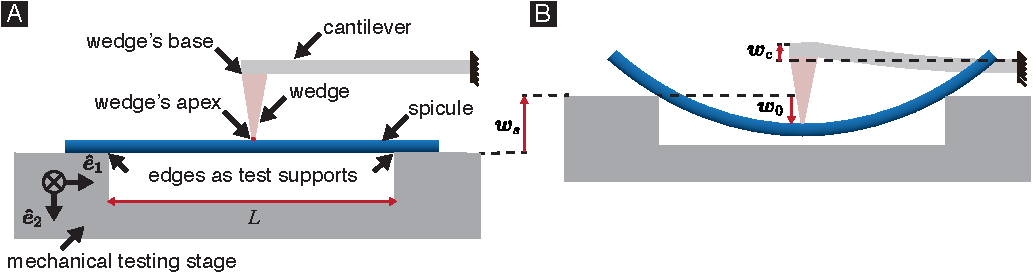
\includegraphics[width=1\textwidth]{../Figures_Submit/SSsetup_V4.pdf}\caption{\label{fig:SSsetup}
An illustration of the simply-supported setup. % hk done
$\subf{A}$
Schematic of the experimental setup used in our recent study~\cite{Sayaka2021Sawtooth} for testing spicules in a simply-supported setup. % hk done
The mechanical testing stage consisted of a stainless steel plate with a~$L~\mu$m wide trench, where the trench edges served as the test's supports. % hk done
The loading device consisted of a wedge attached to a cantilever; to ensure that the
cantilever's right end remained fixed in space during the experiment,
the right end was encastered into a rigid aluminum frame (not shown
in the schematic) that was independent of all the other testing structures. % hk done
$\subf{B}$ Schematic of a simply-supported spicule in our experiment, which is
being deformed under some applied load. % hk done
The loading of the spicules was achieved by displacing the mechanical testing stage by~$w_s~\mu$m
($\physws=-w_s\physe_2$) as shown, where the mechanical testing stage
was mounted onto a three-axis motorized translation stage (not shown
in the schematic) to enable precise control of its motion. % hk done
As a result, the midpoint of the spicule is deflected by~$w_0~\mu$m ($\physwo=w_0\physe_2$)
and the free end of the cantilever is deflected by~$w_c~\mu$m ($\physwc=-w_c\physe_2$). % hk done
For more details on the experiments
see~$\S$\ref{sec:experiment}. % hk done
}
\end{figure}

In this section we briefly recall the set-up of the simply-supported
(SS) experiments mentioned in~$\S$\ref{sec:Introduction}.

A trench of width~$\ndL~\mu$m was cut into a stainless steel mechanical
testing stage (MTS) (see Figure~\ref{fig:SSsetup}$\subf{C}$. The
non-dimensional trench width~$\ndL$ was $1278\pm3$ (mean $\pm$ standard deviation) in
the experiments. Spicules were placed across the trench with their
lengths parallel to the~$\physe_1$ direction\sout{. That is,}\textcolor{red}{so that} initially\textcolor{red}{,}
the spicule's cross-sections were normal to~$\physe_1$. The trench's
edges, which run parallel to the~$\physe_3$ direction, served as
the test's supports. A cantilever with a wedge attached to it was
positioned over the spicule. The wedge's triangular faces were normal
to the~$\physe_3$ direction with the triangle's base normal to the~$-\physe_2$
direction and facing away from the spicule, and the triangle's apex
facing the spicule. At the beginning of the experiment, the wedge's
apex (shown marked in Figure~\ref{fig:SSsetup}$\subf{C}$) was just
above the spicule's midpoint, i.e., over the spicule cross-section
that lay midway across the trench. The cantilever and the wedge were
made of either steel or aluminum.

The loading phase of the tests were conducted by moving the MTS in
the~$-\physe_2$ direction at a rate of~$1~\rm\mu m/sec$.
\textcolor{red}{The MTS was driven by a DC servo motor, whose motion was controlled through a PID algorithm. The stage was moved in  $2~\mu \rm m$ increments. During the increment, the stage's velocity was maintained between ~$50$ and $200~\mu \rm m/sec$. Thus, each  stage increment took anywhere between $10$ and $40~\rm{ms}$. After each increment, the stage was held motionless so that there was a $2100~\rm{ms}$ time interval  between the starting points of any two consecutive increments. Each data point that we report was calculated using the  average value of the sensor readings collected over the last $100~\rm{ms}$ of each of those time intervals.
}

We denote
an arbitrary time instance during the experiment as~$\tau~\text{ms}$,
where~$\tau\in [0,\tau^*]$. The time~$\tau$~=~0 corresponds to
the instance at which the spicule first makes contact with the wedge's
apex, and the time~$\tau=\tau^*> 0$ corresponds to the instance
when the spicule fails. We express the MTS's displacement as~$-w_s(\tau)\physe_2$.
Here,~$w_s(\tau)\in\mathbb{R}$ is a known non-dimensional quantity
since the stage's displacement was an input in our experiment.

As the stage moved upwards ($-\physe_2$ direction) the spicule made
contact with the wedge's apex and got deflected into the trench, while
the cantilever got deflected away from the trench. We express the
cantilever's wedge's motion as~$-w_c(\tau)\physe_2${{}
(compare Figures}~\ref{fig:SSsetup}$\subf{C}${{}
and}~{}{$\subf{D}$}{).
Here,}~{}$w_c(\tau)${{} is the non-dimensional
cantilever displacement, which is defined as the dot product between~}{$-\physe_2$}{{}
and the wedge's displacement vector at the time instance~}{$\tau$}{.}
We denote the spicule's midpoint deflection, or simply displacement,
as~$w_0(\tau)\physe_2$, where~$w_0(\tau)\in\mathbb{R}$ is the
dot product between~$\physe_2$ and the displacement vector of the
centroid of the spicule's cross-section that is directly underneath
the wedge's apex. It can be shown that the quantities~$w_s(\tau)$,~$w_c(\tau)$,
and~$w_0(\tau)$ are related as

\begin{equation}
w_{s}(\tau)=w_{c}(\tau)+w_{0}(\tau).
\label{eq:disp}
\end{equation}In terms of

\begin{subequations}
\label{eq:ndDisps}
\noindent\begin{tabularx}{\textwidth}{@{}X@{}X@{}X@{}X@{}}
\begin{equation}
\label{eq:wshat}\hat{w}_s(\tau) :=\frac{w_s(\tau)}{\ndL} ,
\end{equation}
&
\begin{equation}
\label{eq:wchat}
\hat{w}_c(\tau) :=\frac{w_c(\tau)}{\ndL},
\end{equation}
&
\begin{equation}
\label{eq:w0hatDef}
\hat{w}_0(\tau) :=\frac{w_0(\tau)}{\ndL},
\end{equation}
\end{tabularx}
\end{subequations} equation~\eqref{eq:disp} reads

\begin{equation}
\hat{w}_{s}(\tau)=\hat{w}_{c}(\tau)+\hat{w}_{0}(\tau).
\label{eq:dispND}
\end{equation}

Let~$\u{F}(\tau)$ be the force acting on the spicule's midpoint.
We assume that the wedge's apex only applies force in the~$\pm\physe_2$
directions. This allows us to express

\begin{equation}
\u{F}(\tau)=F(\tau)\physf_{2},\label{eq:Fvec}
\end{equation}
where~$F(\tau)\in\mathbb{R}$ is a non-dimensional quantity. We model
the cantilever as a linear spring that is oriented in the~$\physe_2$
direction and having a stiffness of~$\physkc=\ndkc~\rm mN/\mu m$.
From this model, it follows that

\begin{subequations}
\begin{align}
\label{eq:forcen1}
F(\tau)&=k_{c}w_{c}(\tau).
\intertext{We measured $\ndkc$  independently, using a procedure unrelated to the SS experiments, and found it to vary from $86.4$ to $90.1$ (see Tables S1--S2 of~\cite{Sayaka2021Sawtooth}). The constitutive law expressed by~\eqref{eq:forcen1} can alternately be written as}
\label{eq:force}
\hat{F}(\tau)&=\hat{k}_c\hat{w}_c(\tau),
\end{align}
\end{subequations}where

\begin{subequations}
\noindent\begin{tabularx}{\textwidth}{@{}X@{}X@{}X@{}X@{}}
\begin{equation}\label{eq:Fhat}\hat{F}(\tau) :=\frac{ F(\tau)\ndL^2}{EI},\end{equation} &
\begin{equation}\label{eq:kc}\hat{k}_c :=\frac{k_c\ndL^3}{E I},\end{equation}\\
\end{tabularx}
\end{subequations}~$\ndE~\rm mN/\mu m^2$ is the spicule specimen's Young's modulus,
and~$\ndI~\mu m^4$ is the spicule specimen\textquoteright s bending
moment of inertia.

In each experiment, we measured the function~$\mathbb{R}_{\ge0}\ni\tau\mapsto  w_c(\tau)\in\mathbb{R}$.
Since we knew~$k_c$, on account of~\eqref{eq:wchat} and~\eqref{eq:force},
this was tantamount to measuring the function~$\tau\mapsto\hat{F}(\tau)$.
Additionally, since we know~$w_s(\cdot)$, using the measured~$w_c(\cdot)$
along with~\eqref{eq:wshat},~\eqref{eq:wchat}, and~\eqref{eq:dispND},
we can construct~$\tau\mapsto\hat{w}_0(\tau)$. We call the map

\begin{equation}
\tau\,\stackrel{\gamma_{\text{m}}}{\mapsto}\pr{\hat{w}_{0}(\tau),\hat{F}(\tau)},\label{def:MeasuredForceDisplacementCurveND}
\end{equation}the measured force-displacement curve.

\begin{figure}
\centering{}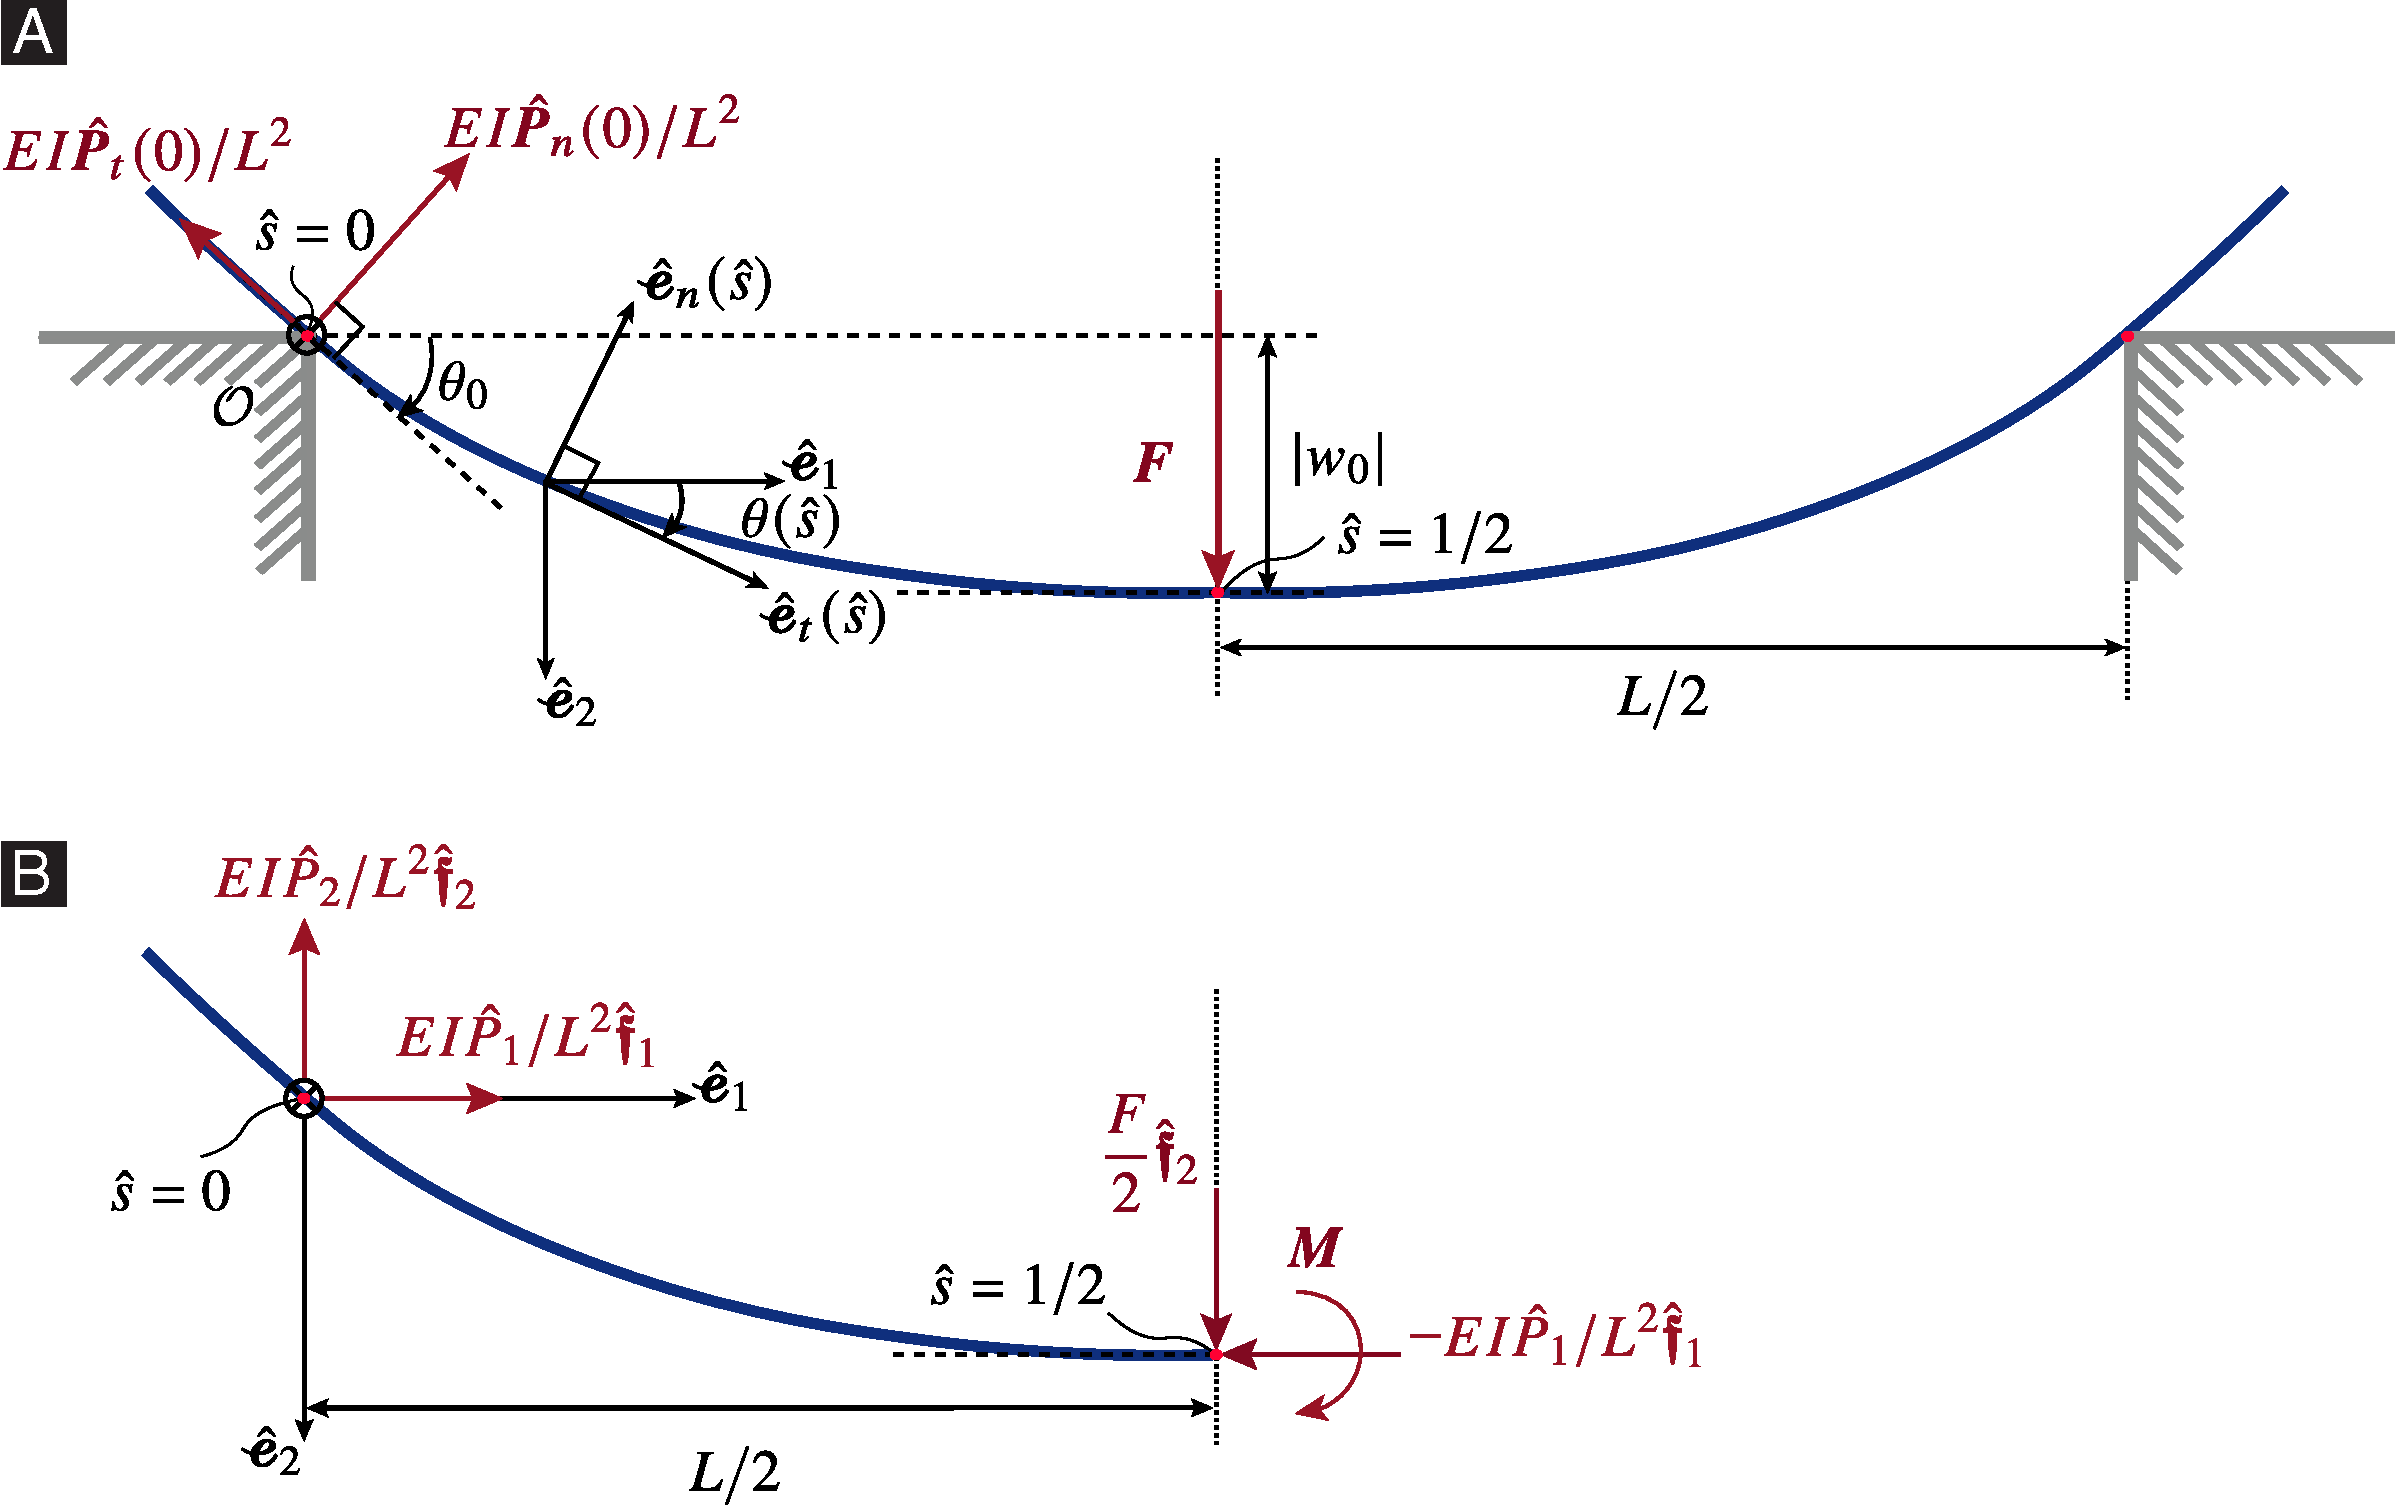
\includegraphics[width=1\textwidth]{../Figures_Submit/BeamSchematic_V15.pdf}
\caption{
\label{fig:BeamSchematic}
Geometry in our mechanics model. % hk done
$\subf{A}$ A schematic of a beam (blue) suspended over a trench (gray). % hk done
% The vectors $\physe_n (0)$ and $\physe_t (0)$, respectively, are normal and tangent to the deformed spicule at the left trench, i.e., at $\hat{s}=0$. % hk done
At~$\hat{s} = 0$ the beam  experiences the normal reaction
force~$E I\chat{\u{P}}_n(0)/L^2$ and the
frictional reaction force~$E I\chat{\u{P}}_t(0)/L^2$. % hk done
The force~$\u{F}$ acts at the spicule midpoint. % hk done
The magnitude of the beam's midpoint's deflection is~$|w_0|$. % hk done
The angle between~$\physe_1$ and~$\physe_{t}\pr{\hat{s}}$ is~$\theta\pr{\hat{s}}$, and~$\theta_0 :=\theta(0)$. % hk done
$\subf{B}$ A free body diagram of the left half of the beam (blue). % hk done
The beam is subject to the
forces~$E I\hat{P}_1/L^2\physf_1$, and $E I\hat{P}_2/L^2\physf_2$ at~$\hat{s} = 0$,
and the forces~$-E I\hat{P}_1/L^2\physf_1$, and $F/2\physf_{2}$ at $\hat{s}=1/2$. % hk done
At $\hat{s}=1/2$ the beam is also subject to a moment $\u{M}$. % hk done
}
\end{figure}

\section{Theory\label{sec:results}}

The goal of the model we develop in this section is to provide a prediction
for the measured force-displacement curves in the loading phase of the
SS experiments.

\subsection{Equations governing the spicule's equilibrium configurations\label{subsec:Governing-equations-of}}

{We denote the total length of the spicule specimen
lying between the supports in the deformed configuration}~{}{$S~\mu$m}{{}
(see Figure~\hypersetup{linkcolor=red}\ref{fig:slip2}\hypersetup{linkcolor=blue}}{$\subf{B}$$\subf{ii}.1$}{).}
We take our problem to be completely symmetric about the trench's
mid-plane. For a given total spicule length,~$S$, we define a spicule's
equilibrium configuration to be a kinematically admissible spicule
deformation map and a spicule-trench edge contact force. The map should
be such that the net force and the moment vanish on every one of the spicule's
material regions; the contact force should be such that it satisfies the
prescribed contact constitutive law between the spicule and the trench.

\subsubsection{Euler's elastica theory\label{subsec:Euler's-Elastica-theory}}

{We assume the spicule to be inextensible. Thus,~}{$S$}{{}
 denotes the total length of the spicule specimen lying between the
supports in its reference configuration as well. We call the length
of the spicule-section lying between a spicule material particle on
the spicule's central axis and the spicule cross-section contacting
the trench's left edge the particle's arc-length coordinate~$s\in (0,S)$
({see Figure~\hypersetup{linkcolor=red}\ref{fig:slip2}\hypersetup{linkcolor=blue}}{$\subf{B}.(ii).2$}).
When there is no risk of confusion, we will henceforth be referring
to a spicule material particle lying on the spicule's central axis
simply as a spicule material particle. We call

\begin{equation}
\label{eq:shat}
\hat{s}:=s/S,
\end{equation}the particle's scaled arc-length coordinate.{{} We
identify a} spicule material particle with either its arc-length or
scaled arc-length coordinate.

As mentioned before, we assume that our problem is completely symmetric
about the trench's mid-plane, i.e., the plane perpendicular to~$\physe_1$
and containing the point~$(\ndL/2,0,0)$. Therefore,
the spicule's deformed shape can be described using the (scaled) deformation
mapping

\begin{subequations}
\begin{equation}
\hat{\u{\alpha}}(\cdot):(0,1/2)\to\mathbb{E},
\end{equation}
where
\begin{equation}
\hat{\u{\alpha}}\pr{\cdot} =\frac{\u{\alpha}\pr{\cdot}}{\ndL} ,
\end{equation}
\label{eq:Alphahat}
\end{subequations}
and~$\u{\alpha}\pr{\xi}$ is the position vector
of the spicule material particle whose arc-length coordinate is~$\xi S$.

We can define a Frenet--Serret frame~\cite{forsyth1912lectures}
corresponding to the curve~$\hat{\u{\alpha}}(\cdot)$
at each spicule material particle. The unit tangent and normal vectors
in that frame at the material particle~$\hat{s}$ can be computed
as

\begin{subequations}
\begin{align}
\label{eq:Tvec}
\physe_{t}\pr{\hat{s}}&=\hat{\u{\alpha}}'\pr{\hat{s}}/\norm{\hat{\u{\alpha}}'\pr{\hat{s}}},\\
\label{eq:Nvec}
\physe_{n}\pr{\hat{s}}&=\physe_{t}'\pr{\hat{s}}/\norm{\physe_{t}'\pr{\hat{s}}},
\end{align}
\end{subequations}respectively, where~$\hat{\u{\alpha}}'\pr{\cdot}$ is the derivative
of~$\hat{\u{\alpha}}\pr{\cdot}$, and~$\physe_{t}'\pr{\cdot}$ is
the derivative of~$\physe_{t}\pr{\cdot}$. Using the definition of~$s$,
the equations~\eqref{eq:shat}, and~\eqref{eq:Alphahat}, it can
be shown that~$\norm{\hat{\u{\alpha}}'\pr{\hat{s}}} =\hat{S}${,
where}\begin{equation}\label{eq:Shat}
\hat{S} =\frac{S}{\ndL}  .\end{equation}

Let~$\theta\pr{\cdot}:(0,1/2)\to (-\pi,\pi]$
be defined such that~$\theta\pr{\hat{s}}$ is
the angle between~$\physe_1$ and~$\physe_{t}\pr{\hat{s}}$\footnote{To be clear, considering two vectors of unit magnitude~$\u{a} := a_1\physe_1 + a_2\physe_2$
and~$\u{b}:=b_1\physe_1 + b_2\physe_2$, the angle between them is
the real number~$\theta$ in~$(-\pi,\pi]$ such that~$a_1\cos(\theta)- a_2\sin(\theta) = b_1$
and~$a_2\cos(\theta) + a_1\sin(\theta) = b_2$.} (see Figure~\ref{fig:BeamSchematic}$\subf{A}$). We can express~$\physe_{t}\pr{\hat{s}},\,\physe_{n}\pr{\hat{s}}$
using~$\theta(\hat{s})$ as

\begin{subequations}
\begin{align}
\label{eq:Tangent}
\physe_{t}\pr{\hat{s}}&=\cos(\theta(\hat{s}))\physe_{1}+\sin(\theta(\hat{s}))\physe_{2},\\
\label{eq:Normal}
\physe_{n}\pr{\hat{s}}&=\sin(\theta(\hat{s}))\physe_{1}-\cos(\theta(\hat{s}))\physe_{2},
\end{align}
\end{subequations}respectively. Let~$\ndE\ndI\chat{\u{P}}(\hat{s})/\ndL^2\in\mathbb{F}$
be the force acting on the spicule cross-section containing the spicule
material particle~$\hat{s}$. Specifically,~$\ndE\ndI\chat{\u{P}}(0)/L^2$
is the force acting on the spicule due to its contact with the trench's
left edge. The vector~$\chat{\u{P}}\pr{0}$ can
be expressed as

\begin{equation}
\chat{\u{P}}\pr{0}
=
\hat{P}_{1}\physf_{1}
+
\hat{P}_{2}\physf_{2},
\label{eq:P12at0}
\end{equation} where~$\hat{P}_1,~\hat{P}_2\in\mathbb{R}$.

The spicule's high aspect ratio and the observation of large displacements
in our SS experiments motivates us to use the Euler's
elastica theory~\cite{euler1952methodus,Timoshenko2009Theory}
to model the spicule's deformation. The elastica theory is an extension
of the EB theory to the regime of large displacements and rotations.
As per the elastica theory, the spicule's cross-sectional rotation~$\theta(\cdot)$
needs to satisfy the non-linear differential equation

\begin{subequations}
\begin{equation}
\theta''(\hat{s})/\hat{S}^{2}+\hat{P}_{1}\sin(\theta(\hat{s}))-\hat{P}_{2}\cos(\theta(\hat{s}))=0,
\label{eq:Elastica}
\end{equation}
over the domain $(0,1/2)$ and satisfy the boundary conditions
\begin{align}
\label{eq:BC1}
\left.\theta'(\hat{s})\right|_{\hat{s}=0}&=0,\\
\label{eq:BC2}
\left.\theta(\hat{s})\right|_{\hat{s}=1/2}&=0.
\end{align}
\label{eq:BVP}
\end{subequations}In~\eqref{eq:BVP},~$\theta'(\cdot)$ and~$\theta''(\cdot)$
denote~$\theta(\cdot)$'s first and second derivatives,
respectively. The boundary condition~\eqref{eq:BC1} follows from
the fact that there is no bending moment acting on the spicule at~$\hat{s} = 0$,
and the boundary condition~\eqref{eq:BC2} follows from the problem's
symmetry about the trench's mid plane.

\subsubsection{Coulomb friction model}

Let

\begin{subequations}
\begin{align}
\label{eq:ftstau}
\physf_{t}(\hat{s}):=
&\mathfrak{F}\pr{\physe_{t}(\hat{s})}=\cos(\theta(\hat{s}))\physf_{1}+\sin(\theta(\hat{s}))\physf_{2},\\
\label{eq:fnstau}
\physf_{n}(\hat{s}):=
&\mathfrak{F}\pr{\physe_{n}(\hat{s})}=\sin(\theta(\hat{s}))\physf_{1}-\cos(\theta(\hat{s}))\physf_{2}.
\end{align}
\label{eq:TangentNormalForces}
\end{subequations}The linear map~$\mathfrak{F}$ appearing in~\eqref{eq:TangentNormalForces}
has been defined in~$\S$\ref{sec:notion}. Using~$\physf_{t}(\hat{s})$,~$\physf_{n}(\hat{s})$,
we can express~$\chat{\u{P}}(\hat{s})$ as the sum of~$\chat{\u{P}}_{t}(\hat{s})$
and~$\chat{\u{P}}_{n}(\hat{s})$, where~$\chat{\u{P}}_{t}(\hat{s})=\hat{P}_{t}(\hat{s})\physf_{t}(\hat{s})$,~$\chat{\u{P}}_{n}(\hat{s})=\hat{P}_{n}(\hat{s})\physf_{n}(\hat{s})${,
and}~$\hat{P}_{t}(\cdot),~\hat{P}_{n}(\cdot): (0,1/2)\to\mathbb{R}$.
We refer to~$\chat{\u{P}}_t(\hat{s})$ and~$\chat{\u{P}}_n(\hat{s})$
as, respectively, the (scaled) tangential and normal forces at the
material particle~$\hat{s}$. We call~$\chat{\u{P}}_t(0)$ and~$\chat{\u{P}}_n(0)$
the (scaled) tangential and normal contact forces (at the left trench
edge), respectively, and for brevity, denote their magnitudes, i.e.,~$\hat{P}_{t}(0)$
and~$\hat{P}_{n}(0)$, as~$\hat{P}_{t}$ and~$\hat{P}_{n}$, respectively.

We define the angle~$\beta_0\in (0,\pi)$ such that

\begin{equation}
\cot\pr{\beta_0} =\frac{\hat{P}_{t}}{\hat{P}_{n}}.
\label{eq:Beta0Def}
\end{equation}It follows from equations~\eqref{eq:P12at0},~\eqref{eq:TangentNormalForces},
and~\eqref{eq:Beta0Def}, and the definitions of~$\hat{P}_{t}$
and~$\hat{P}_{n}$ that

\begin{subequations}
\begin{align}
\hat{P}_{1}&=\hat{P}_{n}\csc\pr{\beta_0}\cos\pr{\theta_0-\beta_0},
\label{eq:P1}
\\
\hat{P}_{2}& =\hat{P}_{n}\csc\pr{\beta_0}\sin\pr{\theta_0-\beta_0},
\label{eq:P2}
\\
\intertext{where}
\label{eq:Theta0}
\theta_{0}&:=\theta(0).
\end{align}
\label{eq:P1P2intoPn}
\end{subequations}

Substituting~$\hat{P}_{1}$,~$\hat{P}_2$ from~\eqref{eq:P1P2intoPn}
into~\eqref{eq:Elastica} and simplifying, we get that

\begin{equation}
\label{eq:Elastica-Scaled}
\theta''(\hat{s})+\hat{S}^2\hat{P}_n\csc\pr{\beta_0}\sin(\theta(\hat{s})-\theta_{0}+\beta_{0})=0.
\end{equation}

We model contact between the spicule and the trench edges using the
Coulomb's law of friction~\cite{popov2017coulomb}. As per the Coulomb's
law, when~$\hat{P}_{n}\ge 0$,~$\left|\hat{P}_{t}\right|\le\mu\hat{P}_{n}$,
which in terms of~$\beta_0$ reads

\begin{equation}
-\mu\le\cot\pr{\beta_0}\le\mu,
\label{eq:CoulombLaw}
\end{equation}where~$\mu$ is the coefficient of friction. (As we
mentioned in~$\S$\ref{sec:Introduction}, in our problem we take
the static and kinetic coefficients of friction to have the same value).

\subsection{Equilibrium force-displacement curves\label{subsec:Equilibrium-force-displacement}}

\subsubsection{Solution to the boundary value problem~\eqref{eq:BVP} using the
solution to the nonlinear pendulum problem\label{subsec:Solution-to-the}}

Following Blasius~\cite[for accessible references, see, e.g.,][]{goldstein1938modern,klamkin1962transformation},
we construct the solution to our boundary value problem (BVP)~\eqref{eq:BVP}
using the solution of an auxiliary initial value problem (IVP).

The IVP we consider is as follows. The function~$\beta:(0,1/2)\to (-\pi,\pi]$
satisfies the nonlinear ordinary differential equation (ODE)


\begin{subequations}
\begin{equation}
\label{eq:pendulum}
\beta''(\hat{s})+\omega^{2}\sin(\beta(\hat{s}))=0,
\end{equation}
and the initial conditions
\begin{align}
\label{eq:PenIC1}
\left.\beta(\hat{s})\right|_{\hat{s}=0}&=\beta_{0},\\
\label{eq:PenIC2}
\left.\beta'(\hat{s})\right|_{\hat{s}=0}&=0,
\end{align}
\label{eq:IVP}
\end{subequations}where~$\omega > 0 $ and~$\beta_0\in (0,\pi)$. The IVP~\eqref{eq:IVP}
is related to the problem of a simple pendulum executing finite angle
motions in a plane. The complete solution to the IVP~\eqref{eq:IVP}
is commonly attributed to Euler~\cite{euler1750novo}. For more modern
references of the solution, see, e.g.,~\cite{whittaker1937treatise,belendez2007exact}.
In order to explicitly note the dependence of the solution to the
IVP~\eqref{eq:IVP}, i.e.,~$\beta(\cdot)$, on the parameters~$\omega$
and~$\beta_{0}$, we denote~$\beta(\cdot)$ in the remainder of this
paper as~$\beta(\cdot;\omega,\beta_0)$ and express it as

\begin{equation}
\beta\left(\hat{s};\omega,\beta_{0}\right)=2\arcsin\left(\sin\frac{\beta_{0}}{2}\ \text{cd}\left(\omega\,\hat{s};\sin^{2}\frac{\beta_{0}}{2}\right)\right),\label{eq:PendulumSol}
\end{equation}
where~$\text{cd}(u; m) :=\cos(\psi(u;m))\pr{1 - m\sin^2(\psi(u;m))}^{-1/2}$
is the Jacobi elliptic function. Here,~$\psi(u;m)$ is the Jacobi
amplitude, which is the inverse of the elliptic integral of the first
kind, i.e.,~$\psi,\, u ,\,m$ satisfy the equation~$u =\int_0^\psi\pr{1 - m^2\sin(\zeta)^2}^{-1/2}\, d\zeta$.

It can be shown that the solution to our BVP,~$\theta(\cdot)$, can
be constructed using~$\beta\left(\cdot;\omega,\beta_{0}\right)$
as

\begin{subequations}
\begin{align}
&\theta(\hat{s})
=
\beta\left(\hat{s};\omega\pr{\hat{S},\hat{P}_{n},\beta_0},\beta_{0}\right)-\beta\left(\frac{1}{2};\omega\pr{\hat{S},\hat{P}_{n},\beta_0},\beta_{0}\right),
\intertext{where}
&\omega\pr{\hat{S},\hat{P}_{n},\beta_0} :=\hat{S}\pr{\hat{P}_n\csc\pr{\beta_0}}^{1/2}.\label{eq:omegaP1}
\end{align}
\label{eq:ThetaSolP1}
\end{subequations}

It can be deduced from~\eqref{eq:ThetaSolP1} that~$\theta(\cdot)$
depends on the independent parameters~$\hat{S}$,~$\hat{P}_n$,
and~$\beta_0$. We will explicitly note this dependence by denoting~$\theta(\cdot)$
as~$\theta(\cdot;\hat{S},\hat{P}_n,\beta_0)$. In order to make our
results look less cumbersome, we will denote the sequence of independent
parameters~$\hat{S}$,~$\hat{P}_n$, and~$\beta_0$ simply as~$\idp$.
In terms of~$\idp$, the solution~$\theta(\cdot;\hat{S},\hat{P}_{n},\beta_0)$
will appear as~$\theta(\cdot;\idp)$, and the result~\eqref{eq:ThetaSolP1}
will read

\begin{subequations}
\begin{align}
\theta(\hat{s};\idp)
&=
\beta\left(\hat{s};\omega\pr{\idp},\beta_{0}\right)-\beta\left(\frac{1}{2};\omega\pr{\idp},\beta_{0}\right),
\intertext{where}
\omega\pr{\idp} &:=\hat{S}\pr{\hat{P}_n\csc\pr{\beta_0}}^{1/2}.
\label{eq:omegaNew}
\end{align}
\label{eq:ThetaSol}
\end{subequations}

\subsubsection{{Midpoint deflection and force}}

In this section, we present formulae for calculating the midpoint deflection~$\hat{w}_{0}$
and force~$\hat{F}$. As we did with~$\theta(\cdot)$, when we want
to note the dependence of~$\hat{w}_0$,~$\hat{F}$,~$\theta_0$,
and~$\hat{\u{\alpha}}\pr{\cdot}$ on the independent parameters~$\hat{S}$,~$\hat{P}_n$,
and~$\beta_0$ explicitly, we will denote them as~$\hat{w}_0\pr{\idp}$,~$\hat{F}(\idp)$,~$\theta_0(\idp)$
and~$\hat{\u{\alpha}}\pr{\cdot;\idp}$, respectively.

We can express~$\hat{\u{\alpha}}(\hat{s};\idp)$ as~$\hat{x}_1(\hat{s};\idp)\physe_1+\hat{x}_2(\hat{s};\idp)\physe_2$,
where~$\hat{x}_1(\cdot;\idp)$,~$\hat{x}_2(\cdot;\idp)$ are smooth
real valued functions on~ $(0,1/2)$. It follows from~(\ref{eq:Tvec})
and~(\ref{eq:Tangent}) that

\begin{subequations}
\begin{align}
\label{eq:x1p}
\hat{x}_{1}'(\hat{s};\idp)&=\hat{S}\cos(\theta(\hat{s};\idp)),\\
\label{eq:x2p}
\hat{x}_{2}'(\hat{s};\idp)&=\hat{S}\sin(\theta(\hat{s};\idp)).
\end{align}
\end{subequations}

\paragraph{Midpoint deflection}

Integrating~(\ref{eq:x2p}) from~$\hat{s}=0$ to~$\hat{s} = 1/2$,
simplifying the expression~$\int_{0}^{1/2}\hat{x}_{2}'(\hat{s};\idp)\, d\hat{s}$
that appears on the left hand side (LHS) of the resulting equation as~$\hat{x}_{2}(1/2;\idp)-\hat{x}_{2}(0;\idp)$,
and then noting that~$\hat{x}_{2}(1/2;\idp)=\hat{w}_0(\idp)$ and~$\hat{x}_{2}(0;\idp)=0$,
we get that

\begin{align}
\hat{w}_0\pr{\idp}=\hat{S}\int_{0}^{1/2}\sin\pr{\theta\pr{\hat{s};\idp}}\, d\hat{s}.
\label{eq:w0hat}
\end{align}

\paragraph{Midpoint force}

From the balance of external forces acting on the left half of the
spicule specimen (Figure~\ref{fig:BeamSchematic}$\subf{B}$) in
the~$\physf_2$ direction, we get that

\begin{equation}
\hat{F}+2\hat{P}_{2}=0.
\label{eq:ForceBalance0}
\end{equation}Substituting~$\hat{P}_2$ in~\eqref{eq:ForceBalance0} from~\eqref{eq:P2}
and then using~\eqref{eq:omegaNew} and substituting the factor~$\hat{P}_n\csc\pr{\beta_0}$
as~$\omega(\idp)^2/\hat{S}^{2}$, we get\begin{equation}
\hat{F}(\idp)=-2\omega(\idp)^2\sin\pr{\theta_0(\idp)-\beta_0}\frac{1}{\hat{S}^2}.
\label{eq:Fhatpenultimate}
\end{equation} Integrating~\eqref{eq:x1p} from~$\hat{s}=0$ to~$\hat{s} = 1/2$,
simplifying the expression~$\int_{0}^{1/2}\hat{x}_{1}'(\hat{s};\idp)\, d\hat{s}$
that appears on the LHS as~$\hat{x}_{1}(1/2;\idp)-\hat{x}_{1}(0;\idp)$,
noting that~$\hat{x}_{1}(1/2;\idp)=1/2$ and~$\hat{x}_{1}(0;\idp)=0$,
multiplying the resulting equation with~$2/\hat{S}$, and then squaring
the result, we get that

\begin{equation}
\frac{1}{\hat{S}^2}=4\pr{\int_{0}^{1/2}\cos\pr{\theta\pr{\hat{s};\idp}}\, d\hat{s}}^{2}.
\label{eq:LS}
\end{equation}
Substituting the factor~$1/\hat{S}^2$ in~\eqref{eq:Fhatpenultimate}
from~\eqref{eq:LS} and simplifying, we get that

\begin{equation}
\hat{F}\pr{\idp}=8\omega\pr{\idp}^{2}\left(\int_{0}^{1/2}\cos\pr{\theta\pr{\hat{s};\idp}}\ d\hat{s}\right)^{2}\sin\left(\beta_{0}-\theta_{0}\pr{\idp}\right).
\label{eq:FhatSol}
\end{equation}

\begin{figure}
\centering{}
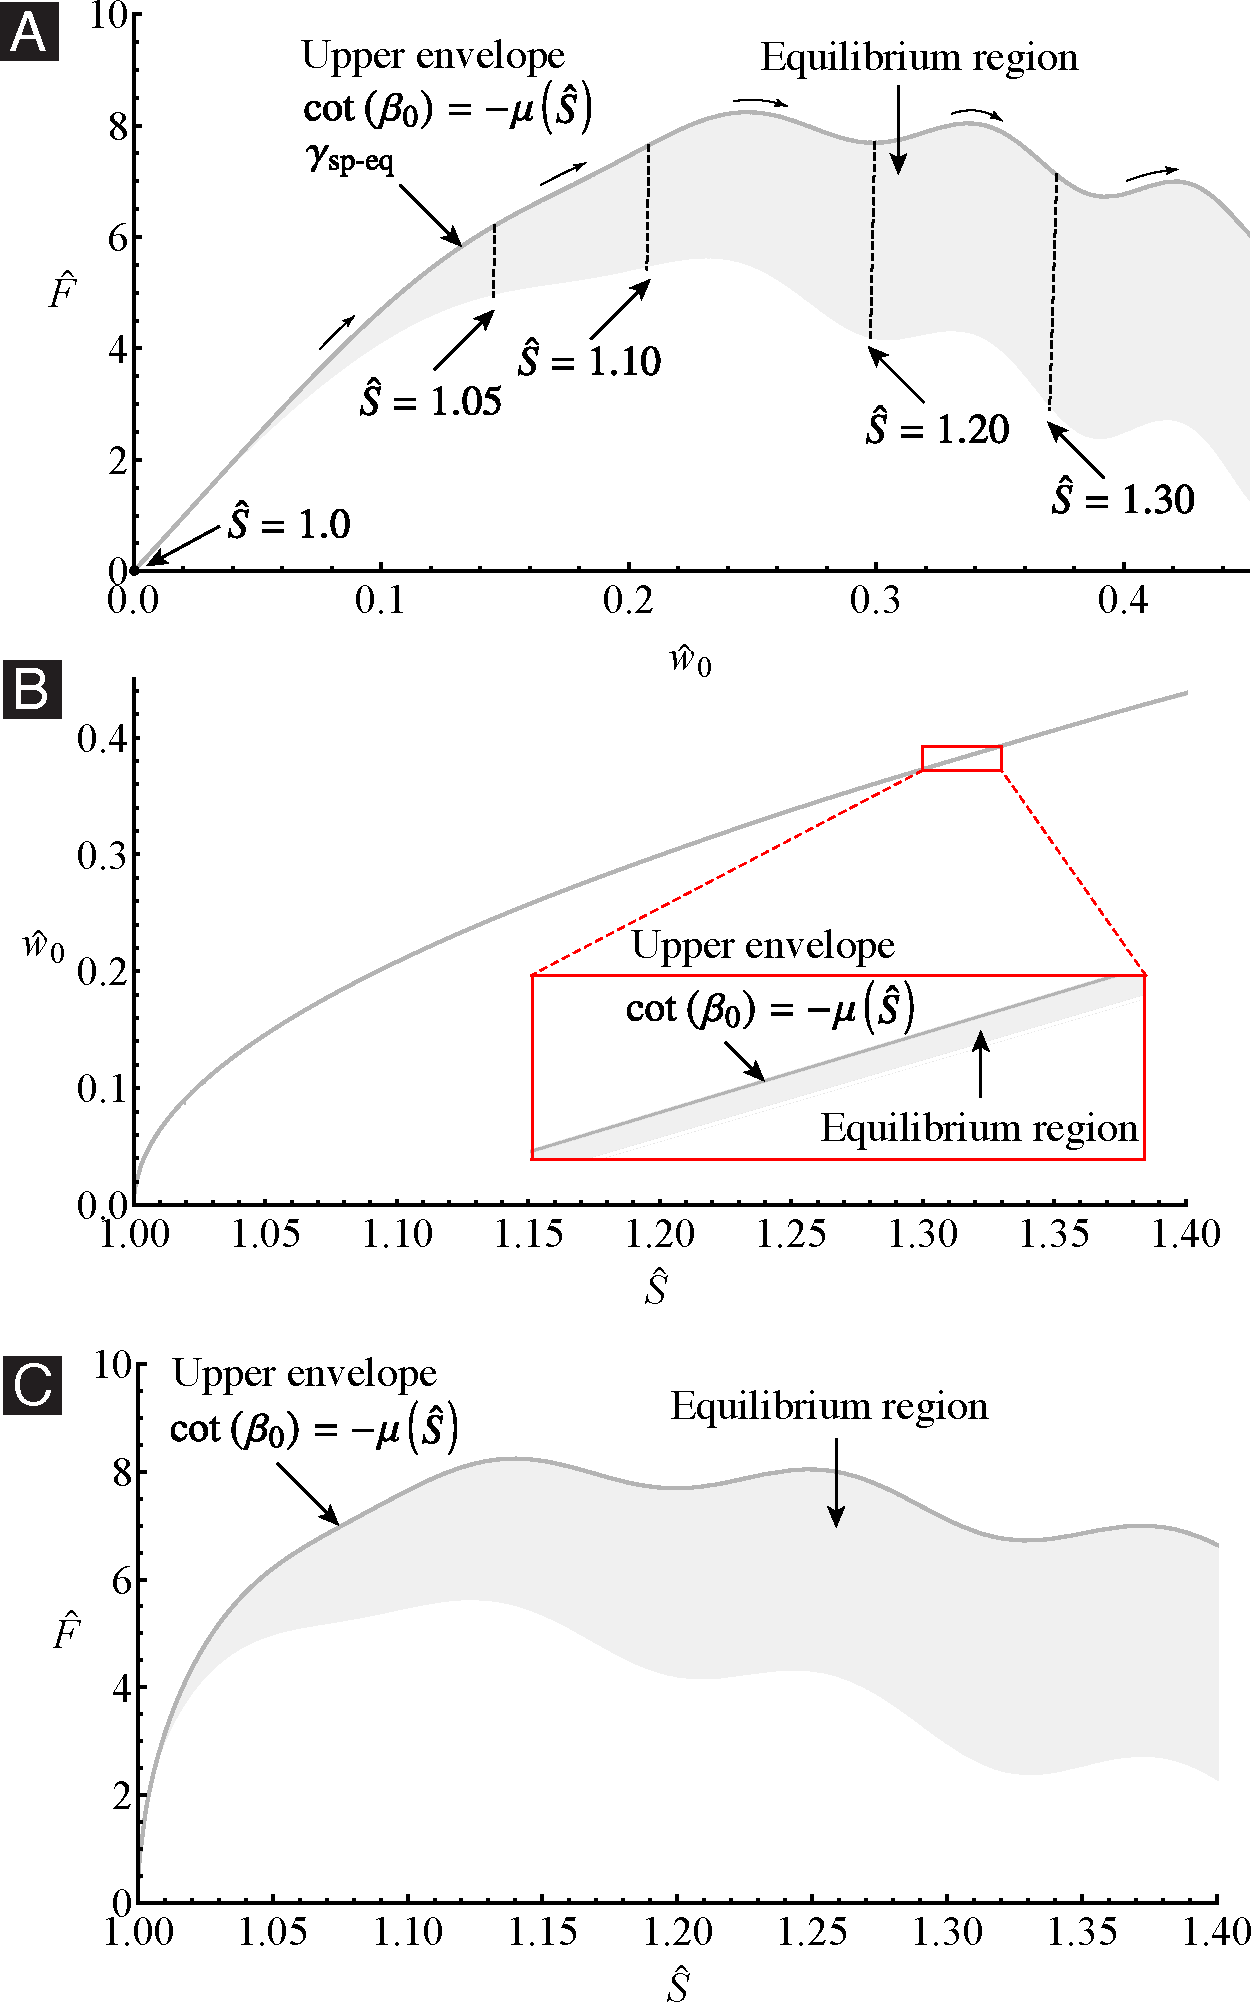
\includegraphics[width=0.9\textwidth]{../Figures_Submit/EquilibriumRegion_V2.pdf}
\caption{(Caption continued on next page)}
\label{fig:EquilibriumRegions}
\end{figure}
\begin{figure}
\centering{}
\contcaption{
The equilibrium region in the~$\hat{w}_0$-$\hat{F}$, $\hat{S}$-$\hat{w}_0$, and $\hat{S}$-$\hat{F}$  space for a representative case. % hk done
We consider the case in which the coefficient
of friction varies as in \eqref{eq:muofS} with $\mu_0=0.3$, $A=0.2$, $\hat{\lambda}=0.02 \pi$, and $\phi=0$, i.e., in which $\mu(\hat{S})=0.3\left(1+0.2\cos\pr{\hat{S}/0.02}\right)$. % hk done
For this case we computed the equilibrium regions using the procedure detailed in Algorithm \ref{algo:equilibrium}. % hk done
Subfigures $\subf{A}$, $\subf{B}$, and $\subf{C}$ show the
  equilibrium region in the~$\hat{w}_0$-$\hat{F}$, $\hat{S}$-$\hat{w}_0$, and $\hat{S}$-$\hat{F}$  space, respectively. % hk done
In each of the subfigures the equilibrium region is shown
in light gray,  while the upper envelope of the equilibrium region (i.e., the equilibrium curve) is shown as a dark-gray curve. % hk done
In~$\subf{A}$ we mark a locus of configurations in which $\hat{S}$ is constant using a dashed black curve. % hk done
The solid arrows above the equilibrium curve indicate that~$\hat{S}$ strictly increases as we travel along the curve starting from the  origin. % hk done
}
\end{figure}

\subsubsection{Compatibility\label{subsec:Compatibility}}

Substituting~$\theta\pr{\cdot;\idp}$ in~\eqref{eq:LS} from~\eqref{eq:ThetaSol}
and rearranging, we get

\begin{equation}
\hat{S}=
\frac{1}{2}\left(\int_{0}^{1/2}\cos\left(\beta\left(\hat{s};\omega(\idp),\beta_{0}\right)-\beta\left(\frac{1}{2};\omega(\idp),\beta_{0}\right)\right)\ d\hat{s}\right)^{-1}.\label{eq:Compatibility}
\end{equation}

\subsubsection{Upper envelope of the equilibrium region and the closing equation\label{subsec:equilibrium}}

In order to derive our model's predictions for the force-displacement
curves measured by the SS experiments in the loading phase, \sout{we need
to first extract} the spicule-specimen's equilibrium configurations \textcolor{red}{first need to be extracted}.
We define what we physically mean by the spicule specimen's equilibrium
configuration at the beginning of~$\S$\ref{subsec:Governing-equations-of}
(when the spicule specimen is in one of its equilibrium configurations,
that does not necessarily mean that the MTS's cantilever wedge is
also in one of its equilibrium configurations, i.e., that our entire
mechanical system is in equilibrium. See~$\S$\ref{subsec:Force-displacement-curves-that}
for further discussion of this issue). Mathematically, a spicule's
equilibrium configuration can be described as an ordered set~$\pr{\hat{S},\hat{P}_{n},\beta_0}$
that satisfies the contact constitutive law~\eqref{eq:CoulombLaw}
and the compatibility condition~\eqref{eq:Compatibility}. We mark
the equilibrium configurations, which \sout{we}\textcolor{red}{were} determined numerically using
Algorithm~\ref{algo:equilibrium}, in the~$\hat{w}_0$-$\hat{F}$,~$\hat{S}$-$\hat{w}_0$,
and~$\hat{S}$-$\hat{F}$ spaces for a representative case in Figures{~\ref{fig:EquilibriumRegions}}$\subf{A}$,~$\subf{B}$,
and~$\subf{C}$, respectively. For a given~$\hat{S}$, there can
exist more than one equilibrium configuration. This is partly because
as can be seen from~\eqref{eq:Beta0Def} and~\eqref{eq:CoulombLaw},
the number~$\cot\pr{\beta_0}$ only needs to lie between certain
bounds, specifically between~$\pm\mu$. Therefore, in general, the
sets of equilibrium states have non-zero measures in the~$\hat{w}_0$-$\hat{F}$,~$\hat{S}$-$\hat{w}_0$
or~$\hat{S}$-$\hat{F}$ spaces.

However, it can be argued that in the loading portion of the SS experiments,~$\hat{P}_{n}\ge 0$.
Under some mild assumptions on the loading rate, it can be further
argued\footnote{The mathematical analysis underlying this assertion is quite involved
and therefore we plan on publishing it elsewhere.} that~$\cot\pr{\beta_0}$ in fact achieves its lower bound, i.e.,
that

\begin{equation}
\cot\pr{\beta_0}=-\mu.
\label{eq:MoreRestrictiveCoulombLaw}
\end{equation}As \sout{we} discussed in~$\S$\ref{sec:Introduction}, it is reasonable
to assume that~$\mu$ varies along the spicule's length\sout{. That is,}\textcolor{red}{~so that}
the value of~$\mu$ depends on the contact position between the spicule
and the trench's left edge, which\sout{, of course,} depends on~$\hat{S}$.
We assume that the dependence of~$\mu$ on~$\hat{S}$ can be expressed
as

\begin{equation}
\mu\pr{\hat{S}}=\mu_{0}\left(1+A\cos\left(\frac{ \pi \hat{S}}{\hat{\lambda}}+\phi\right)\right),\label{eq:muofS}
\end{equation}
where $\hat{\lambda}:=\lambda/L$, $\lambda \in \mathbb{R}_{\ge0}$. Here, $\lambda~\mu$m is the wavelength of the assumed periodic variation of the coefficient of friction. Note that the value of the phase~$\phi$, depending on the positions
of contacting points between the spicule specimens and the trench
edges at the beginning of the experiments, may not be the same as
the value of~$\phi$ in~\eqref{eq:muofS1}.

Therefore, in an equilibrium state, the value of~$\beta_0$ is fully
determined by the value of~$\hat{S}$ in that state. More specifically,
it follows from~\eqref{eq:MoreRestrictiveCoulombLaw} that~$\beta_0$
is equal to the value of~$\beta_0\pr{\hat{S}}$ , where the function~$\beta_0(\cdot):[1,\infty)\to (0,\pi)$
is defined by equations

\begin{subequations}
\begin{align}
\sin\pr{\beta_0\pr{\hat{S}}}&=\frac{1}{\sqrt{1+\mu\pr{\hat{S}}^2}},\\
\cos\pr{\beta_0\pr{\hat{S}}}&=\frac{-\mu\pr{\hat{S}}}{\sqrt{1+\mu\pr{\hat{S}}^2}}.
\end{align}
\label{eq:FrictionLaw}
\end{subequations}As \sout{we }mentioned in~$\S$\ref{sec:Introduction}, for simplicity,
we take~$\mu(\cdot)$ to be of the form given by~\eqref{eq:muofS}.

It now follows from~\eqref{eq:Compatibility} that in the state mentioned
above, the value of~$\hat{P}_n$ is also fully determined by the
value of~$\hat{S}$\textcolor{red}; \sout{. That is, it follows from~\eqref{eq:Compatibility}
that} the value of~$\hat{P}_n$ has to be a root of~$f\pr{\cdot;\hat{S},\beta_0\pr{\hat{S}}}$,
and the function~$f\left(\cdot;\hat{S},\beta_0\right):\mathbb{R}_{\ge 0}\to\mathbb{R}$
is defined by equation

\begin{equation}
f\left(\ensuremath{\cdot};\hat{S},\beta_0\right)=1-2\hat{S}\int_{0}^{1/2}\cos\left(\beta\left(\hat{s};\omega(\hat{S},\cdot,\beta_{0}),\beta_{0}\right)-\beta\left(\frac{1}{2};\omega(\hat{S},\cdot,\beta_{0}),\beta_{0}\right)\right)\ d\hat{s}.
\label{eq:ClosingEquation}
\end{equation}
In general,~$f\pr{\cdot;\hat{S},\beta_0\pr{\hat{S}}}$ will have multiple
roots. However, using practical considerations, it can be deduced
that only the smallest of~$f\pr{\cdot;\hat{S},\beta_0\pr{\hat{S}}}$'s
roots is relevant in the context of the SS experiments. We denote
the value of that smallest root as~$\hat{P}_n\pr{\hat{S}}$, which
can be computed using the Newton-Raphson method.


The results put forward in the last three paragraphs can be summarized
by stating that, during the loading portion of the SS experiments,
the equilibrium states have the form~$\pr{\hat{S},\hat{P}_n\pr{\hat{S}},\hat{\beta}_0\pr{\hat{S}}}$.
We call the set of the equilibrium states having this form the upper
envelope of the equilibrium region (shown as gray curves in Figure~\ref{fig:EquilibriumRegions}).
The upper envelope of the equilibrium region in the~$\hat{w}_0$-$\hat{F}$
space can be expressed as the parametric curve

\begin{subequations}
\begin{align}
\gamma_{\text{sp-eq}}&:=
\left\{\pr{w_{0}^+\pr{\hat{S}},\hat{F}^+\pr{\hat{S}}}~|~\hat{S}\ge 1\right\},
\label{def:GammaEq}
\intertext{where $\hat{w}_0^+(\cdot):[1,\infty)\to\mathbb{R}_{\ge0}$ is defined by the equation}
\hat{w}_0^+\pr{\hat{S}}&=\hat{w}_0\pr{\hat{S},\hat{P}_n\pr{\hat{S}},\hat{\beta}_0\pr{\hat{S}}},
\label{def:hatw0plus}
\intertext{and $\hat{F}^+:[1,\infty)\to\mathbb{R}_{\ge 0}$ is defined by the equation}
\hat{F}^+\pr{\hat{S}}&=\hat{F}\pr{\hat{S},\hat{P}_n\pr{\hat{S}},\hat{\beta}_0\pr{\hat{S}}}.
\label{def:hatFplus}
\end{align}
\label{def:UpperEnvelope}
\end{subequations} We will be referring to~$\gamma_{\text{sp-eq}}$ simply as the spicule
equilibrium curve. The equilibrium curve can be numerically constructed using Algorithm~\ref{algo:equilibrium} after changing line number
5 in it to \textquotedbl Compute~$\beta_{0}^+\leftarrow\text{arccot}\pr{-\mu\pr{\hat{S}}}$,
then~$\beta_{0}^-\leftarrow\beta_{0}^+$\textquotedbl{}

\begin{algorithm}[ht!]
\caption{Procedure for computing the equilibrium region}
\label{algo:equilibrium}
\noindent\begin{minipage}{\textwidth}\renewcommand\footnoterule{}
\begin{algorithmic}[1]
\State{\textbf{Input:} $\mu_0, A,\hat{\lambda},\phi,\hat{S}^*$\footnote{The parameter $\hat{S}^*>1$ specifies the maximum value of $\hat{S}$ among all the computed equilibrium configurations.}, and natural numbers $n_{\hat{S}}$, and $n_{\beta_0}$\footnote{The parameters  $n_{\hat{S}}$ and $n_{\beta_0}$, respectively, specify the number of different  $\hat{S}$ and  $\beta_0$ values among the computed equilibrium configurations.}
}
\State{\textbf{Initialization:} $\hat{S} = 1$, $\hat{P}_n = 0$, $\hat{w}_0 = 0$, $\hat{F} = 0$, $\Delta\hat{S} =\hat{S}^*/n_{\hat{S}}$}
\For{$\hat{S} = 1,1+\Delta\hat{S},1+2\Delta\hat{S},\dotsc,\hat{S}^*$}
\State Compute~$\mu\pr{\hat{S}}\leftarrow\mu_{0}\left(1+A\cos\left(\pi\hat{S}/\hat{\lambda}+\phi\right)\right)$
\State Compute~$\beta_{0}^+\leftarrow\text{arccot}\pr{-\mu\pr{\hat{S}}} $ and $\beta_{0}^-\leftarrow\text{arccot}\pr{\mu\pr{\hat{S}}} $
\State Compute~$\Delta\beta_0\leftarrow\pr{\beta_0^+ -\beta_0^-}/n_{\beta_0}$\For{$\beta_{0}  =\beta_0^-,\beta_0^-+\Delta\beta_0,\beta_0^-+2\Delta\beta_0,\dotsc\beta_0^+$}
\State Solve for~$\hat{P}_{n}$ as the smallest root of~$f(\cdot;\hat{S},\beta_{0})$\footnote{defined in~\eqref{eq:ClosingEquation}}
\State Construct~$\theta(\cdot;\idp)$ from~\eqref{eq:ThetaSol} using $\hat{S}$, $\hat{P}_{n}$,and $\beta_0$
\State Determine~$\hat{w}_0(\idp)$ and~$\hat{F}(\idp)$ from~\eqref{eq:w0hat},~\eqref{eq:FhatSol},~\eqref{eq:omegaNew} and~\eqref{eq:Theta0}
\State Save the points $(\hat{S},\hat{w}_0(\idp))$, $(\hat{S},\hat{F}(\idp))$, and $(\hat{w}_0(\idp),\hat{F}(\idp))$ as respective members of the equilibrium regions in the $\hat{S}$-$\hat{w}_0$, $\hat{S}$-$\hat{F}$, and $\hat{w}_0$-$\hat{F}$ spaces
\EndFor
\EndFor
\State{\textbf{Output:} A collection of $n_{\hat{S}}\times n_{\beta_0}$ equilibrium points in each of the  $\hat{S}$-$\hat{w}_0$, $\hat{S}$-$\hat{F}$, and $\hat{w}_0$-$\hat{F}$ spaces}
\end{algorithmic}
\end{minipage}
\end{algorithm}

\paragraph{Remarks}
\begin{enumerate}
\item \label{enu:Remark1}As can be noted from~\eqref{def:UpperEnvelope},
the curve~$\gamma_{\text{sp-eq}}$ is parameterized by the total
length~$\hat{S}$. The left end of the curve, i.e., the point~$(0,0)$,
corresponds to~$\hat{S}=1$ (see Figure~\ref{fig:EquilibriumRegions}$\subf{A}$).
Thus, the value of~$\hat{S}$ strictly increases as we travel along
the curve starting from the origin.
\item The equilibrium curves from our model for the cases in which~$\mu_0=0.0$
or~0.6 and~$A=0.0$ or~0.4 are shown in Figure~\ref{fig:NBSComparison}$\subf{A}$.
In all cases, as expected, the equilibrium curves predicted by our
model asymptote to the one predicted by the EB theory (see equation~(5) in~\cite{Sayaka2021Sawtooth}) as the midpoint
deflection becomes small.
\item When~$A=0.0$, the most noticeable aspect of the equilibrium curves
from our model is that the force initially increases and \sout{then }later
decreases with the midpoint deflection. In contrast, in the equilibrium
curve predicted by the EB theory (see Figure~\ref{fig:NBSComparison}$\subf{A}$),
the force always increases with the deflection.
\item When~$A\neq0.0$, the equilibrium curves from our model have an undulatory
nature. The sawtooth pattern in our model is a consequence of these
undulations. The undulations appear to become more pronounced as the
values of~$\hat{S}$ and~$\hat{w}_0$ increase, starting from when~$\hat{F}$
is about to reach its maximum value. As noted from Figure~\ref{fig:sawtooth}
in the SS experiments, the sawtooth-pattern appears or is pronounced
in this very same region.
\end{enumerate}

\subsection{Force-displacement curves that will be measured in the simply-supported
experiments\label{subsec:Force-displacement-curves-that}}

\begin{figure}
\centering{}
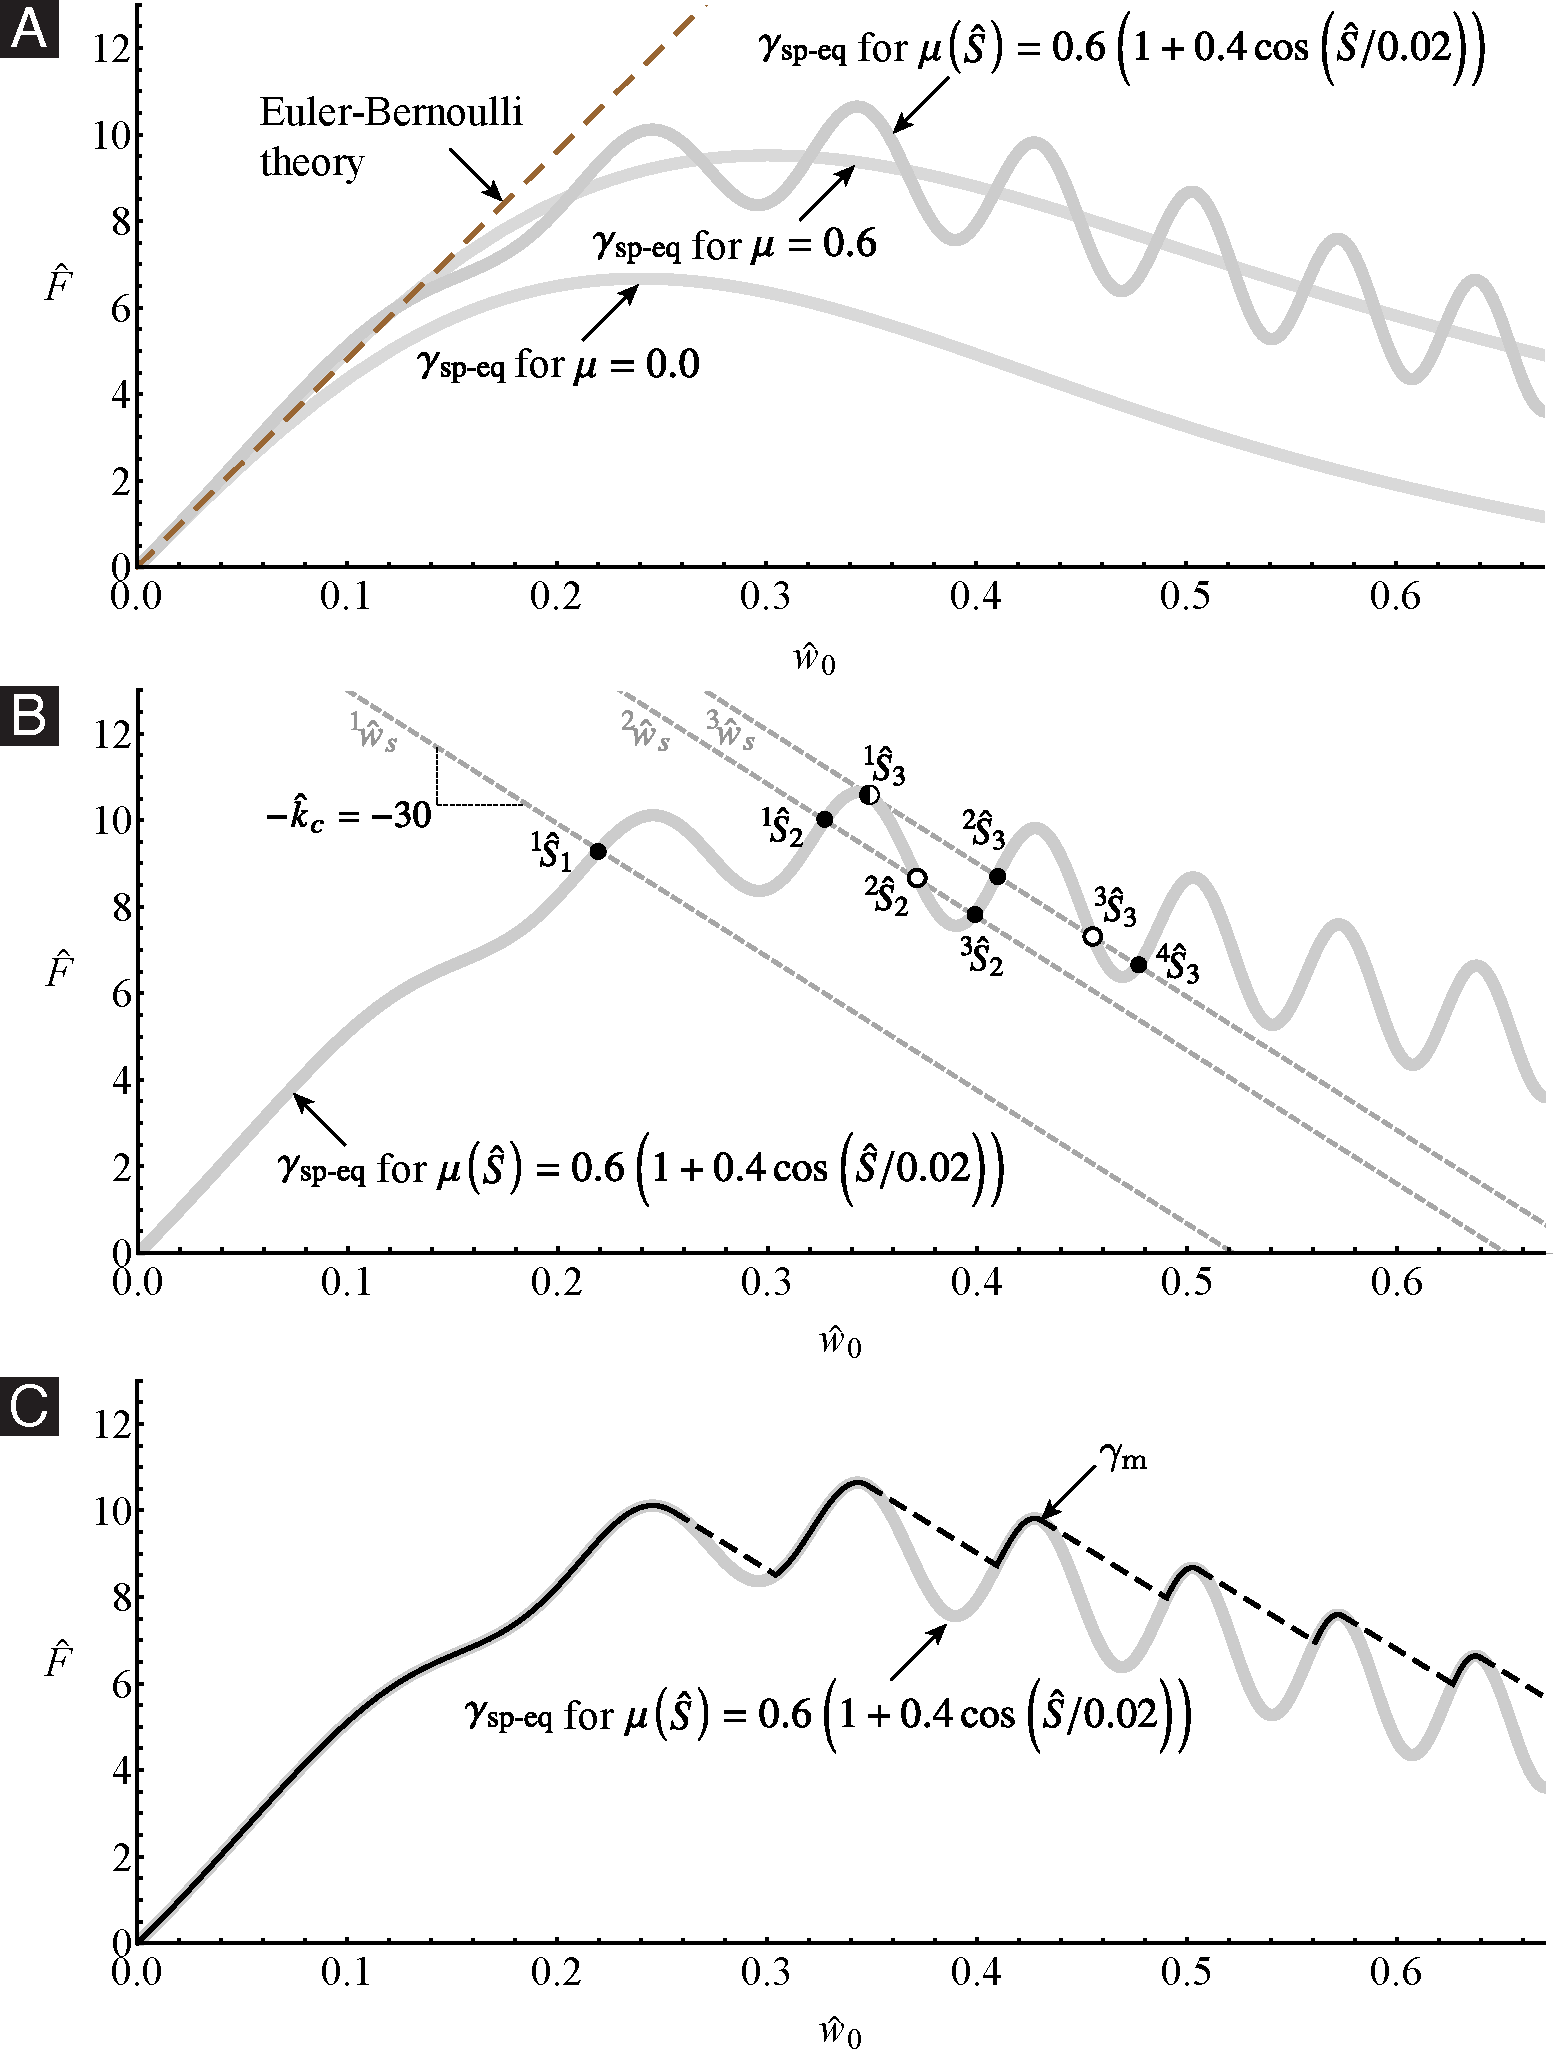
\includegraphics[width=1\textwidth]{../Figures_Submit/Model_V2.pdf}
\caption{(Caption continued on next page)}
\label{fig:NBSComparison}
\end{figure}

\begin{figure}
\centering{}
\contcaption{
Equilibrium and measured force-displacement curves.
$\subf{A}$ shows the equilibrium curves, $\gammaeq$, for the cases $\mu\pr{\hat{S}}=0.6\left(1+0.4\cos\pr{\hat{S}/0.02}\right)$,
$\mu\pr{\hat{S}}=0.6$, and $\mu\pr{\hat{S}}=0.0$, using
gray lines.
The equilibrium curve predicted by the Euler-Bernoulli theory is also shown for reference, using dashed brown lines.
$\subf{B}$ and $\subf{C}$ again show the equilibrium curve corresponding to $\mu\pr{\hat{S}}=0.6\left(1+0.4\cos\pr{\hat{S}/0.02}\right)$.
They only consider this equilibrium curve and a cantilever stiffness of $\hat{k}_c=30$  and show the measured curves for two different $\hat{w}_s(\cdot)$.
$\subf{B}$ considers the $\hat{w}_s(\cdot)$ given in \eqref{eq:DiscontinuousWs} for $\lsc[1]{w}_s$, $\lsc[2]{w}_s$, and $\lsc[3]{w}_s$ equal to 0.52, 0.65, and 0.69, respectively.
In $\subf{B}$, on the equilibrium curve, we mark the  overall-equilibrium configurations at  some three time instances that, respectively, belong to the intervals $(0,\tau_1]$, $(\tau_1,\tau_2]$, and $(\tau_2,\tau_3]$, which appear in \eqref{eq:DiscontinuousWs}.
The stable overall-equilibrium configurations are shown as  filled circles; the unstable configurations as open circles; and the partially-stable  configurations as semi-filled circles.
All overall-equilibrium configurations corresponding to the same time instance are connected using a dashed gray line.
The three dashed gray lines are the graphs of the function~\eqref{def:Fcant} at the three previously mentioned time instances.
The graph of the measured curve in this case consists of  just the three points that are shown marked as $\lsc[1]{\hat{S}}_1$, $\lsc[1]{\hat{S}}_2$, and $\lsc[2]{\hat{S}}_3$.
$\subf{C}$ shows the measured curve~$\gamma_{m}$ for the case  in which $\hat{w}_s(\cdot)$ is some continuous, monotonically increasing function of time.
The measured curve in this case  is the discontinuous curve that is shown using thin black lines.
The straight line segments that span the discontinuities of this curve signify the slip instabilities  occurring at the trench edges.}
\end{figure}

In~$\S$\ref{subsec:equilibrium}, we discussed that only a subset
(specifically, the upper envelope) of the spicule's equilibrium configurations
is relevant in the loading phase of the SS experiments. In the~$\hat{w}_0$-$\hat{F}$
space, we termed that upper envelope~\eqref{def:UpperEnvelope} the
spicule-equilibrium curve,~$\gamma_{\text{sp-eq}}$. The spicule
configurations sampled by the experiment have to necessarily lie on~$\gamma_{\text{sp-eq}}$.
However, not all the configurations in~$\gamma_{\text{sp-eq}}$ will
be sampled during the loading portion of the SS experiment. This is
because the spicule being in equilibrium does not necessarily
mean that the MTS's wedge is in one of its equilibrium configurations.
The force acting on the spicule's midpoint has to be provided by the
wedge's apex (shown marked in Figure~\ref{fig:SSsetup}$\subf{C}$).
However, that force may not necessarily be balanced by the force acting
on the wedge's base due to the MTS's cantilever's deformation.

To be more precise, we analyze the force balance on the wedge of the MTS.
We assume that in the SS experiments, the total length~$\hat{S}$
evolves in the manner dictated by the function~$\hat{S}:[0,\tau^*]\to [1,\infty)$.
As \sout{we} mentioned \textcolor{red}{previously}, the experiment will only sample configurations on~$\gamma_{\text{sp-eq}}$.
At the time instance~$\tau$, the measured midpoint deflection will
be~$\hat{w}_0^{+}\pr{\hat{S}\pr{\tau}}$, i.e.,~$\hat{w}_0(\tau)=\hat{w}_0^{+}\pr{\hat{S}\pr{\tau}}$,
and the measured force acting on the spicule's midpoint will be~$\hat{F}^+\pr{\hat{S}(\tau)}\physf_{2}$,
i.e.,~$\hat{F}(\tau)=\hat{F}^+\pr{\hat{S}(\tau)}$. This force needs
to be provided by the wedge's apex. Therefore, the force acting on the wedge's
apex will be~$-\hat{F}^+\pr{\hat{S}(\tau)}\physf_{2}$. It follows
from~\eqref{eq:dispND} and~\eqref{eq:disp} that the force acting
on the wedge's base is~$\hat{k}_{c}\left(\hat{w}_{s}(\tau)-\hat{w}_{0}^+\pr{\hat{S}\pr{\tau}}\right)\physf_2$,
where\sout{, recall that,}~$\hat{w}_{s}(\cdot)$ prescribes how the stage-displacement
evolves with time during the experiment. Therefore, the equilibrium
condition for the wedge gives that~$\hat{S}(\tau)$ be a root of
the function~$R(\cdot;\tau):[1,\infty)\to\mathbb{R}$,

\begin{subequations}
\begin{align}
R\pr{\hat{S};\tau}&:=\hat{F}_{\rm cant}(\hat{w}_0^{+}\pr{\hat{S}};\tau)-\hat{F}^+\pr{\hat{S}},\\
\intertext{where}
\hat{F}_{\rm cant}(\hat{w}_0;\tau)&:=\hat{k}_c (\hat{w}_s(\tau)-\hat{w}_0).
\label{def:Fcant}
\end{align}
\label{eq:NonDimObliqueLine}
\end{subequations}We will be referring to the point~$\pr{\hat{w}_{0}^{+}\pr{\hat{S}\pr{\tau}},\hat{F}^{+}\pr{\hat{S}\pr{\tau}}}$,
where~$\hat{S}\pr{\tau}$ is a root of~$R(\cdot;\tau)$, an overall-equilibrium
configuration at the time instance~$\tau$. The overall-equilibrium
configurations at the time instance~$\tau$ can be visualized in
the~$\hat{w}_0$-$\hat{F}$ space (see, e.g., Figure~\ref{fig:NBSComparison}$\subf{B}$)
as the intersection points between~$\gamma_{\text{sp-eq}}$ and the
graph of~$\hat{F}_{\rm cant}(\cdot;\tau)$.

\subsubsection{Evolution postulate and our model's prediction for the measured force-displacement
curves\label{subsec:Evolution-postulate-and}}

In order to derive our model's prediction for the measured force-displacement
curve, we consider a thought experiment in which\begin{equation}
\hat{w}_s(\tau)=\left\{
\begin{array}{ll}
\lsc[1]{\hat{w}}_s,&\tau\in(0,\tau_1],\\
\lsc[2]{\hat{w}}_s,&\tau\in(\tau_1,\tau_2],\\
\lsc[3]{\hat{w}}_s,&\tau\in(\tau_2,\tau_3].\\
\end{array}
\right.
\label{eq:DiscontinuousWs}
\end{equation}

In Figure~\ref{fig:NBSComparison}$\subf{B}$, considering a representative~$\hat{k}_c$,
we mark and label the overall-equilibrium configurations at the three
different stage displacements~$\lsc[1]{\hat{w}}_s$,~$\lsc[2]{\hat{w}}_s$,
and~$\lsc[3]{\hat{w}}_s$. As noted from the figure, there can exist
more than one overall-equilibrium configurations at a given stage
displacement. At the stage displacement~$\lsc[1]{\hat{w}}_s$, there
exists only one overall-equilibrium configuration. We denote the total
length in that configuration as~$\lsc[1]{\hat{S}}_1$ and label the
configuration as~$\lsc[1]{\hat{S}}_1$ in Figure~\ref{fig:NBSComparison}$\subf{B}$.
However, at~$\lsc[2]{\hat{w}}_s$, there exist three overall-equilibrium
configurations. As before, we label these configurations in Figure~\ref{fig:NBSComparison}$\subf{B}$
using their total lengths, i.e., as~$\lsc[1]{\hat{S}}_2$,~$\lsc[2]{\hat{S}}_2$,
and~$\lsc[3]{\hat{S}}_2$. At~$\lsc[1]{\hat{w}}_s$, it is clear
that the experiment will measure the total length~$\lsc[1]{\hat{S}}_1$,
i.e.,~$\hat{S}(\tau)=\lsc[1]{\hat{S}}_1$ for all~$\tau\in (0,\tau_1]$.
However, at~$\lsc[2]{\hat{w}}_s$, which one of the three total lengths
will the experiment measure? From a theoretical mechanics perspective,
the question just posed is the same as the one analyzed in~\cite[Section 3 in][]{deng2019effect,kesari2011effective,deng2020angle},
though the mechanical system investigated in~\cite{deng2019effect,kesari2011effective,deng2020angle}
is different from the one studied in this paper. Following the analysis
presented in~\cite{deng2019effect,kesari2011effective,deng2020angle},
a prerequisite for an overall-equilibrium configuration to be measurable
is that it is~$\textit{stable}$. The overall equilibrium state with
total length~$\lsc[j]{\hat{S}}_i$ is stable, iff

\begin{equation}
R'\pr{\lsc[j]{\hat{S}}_i;\tau}=-\hat{k}_c\left.\hat{w}_{0}^{+}\right.'\pr{\lsc[j]{\hat{S}}_i}
-\left.\hat{F}^{+}\right.'\pr{\lsc[j]{\hat{S}}_i}<0.
\label{eq:StabilityCriteria}
\end{equation}

Using~\eqref{eq:StabilityCriteria}, it can be deduced from Figure~\ref{fig:NBSComparison}$\subf{B}$
that~$\lsc[1]{\hat{S}}_2$ and~$\lsc[3]{\hat{S}}_2$ are stable,
while~$\lsc[2]{\hat{S}}_2$ is unstable. However, the question still
remains as to which of~$\lsc[1]{\hat{S}}_2$ and~$\lsc[3]{\hat{S}}_2$
will be measured. \sout{In order to}\textcolor{red}{To} answer this question, as done in~\cite{kesari2011effective},
we postulate that among the different measurable configurations, the
system will evolve into the one that is closest to the last measured
configuration. In the current case, this evolution postulate implies
that the configuration that the system will chose among the measurable
configurations will be the one whose total length is closest to the
one in the last measured configuration. The last measured configuration
in our thought experiment\sout{, of course,} is~$\lsc[1]{\hat{S}}_1$. Therefore,
when the stage displacement is~$\lsc[2]{\hat{w}}_s$, amongst~$\lsc[1]{\hat{S}}_2$
and~$\lsc[3]{\hat{S}}_2$, the experiment will measure the one that
is closer to~$\lsc[1]{\hat{S}}_1$. It follows from remark{~\ref{enu:Remark1}} in~$\S$\ref{subsec:equilibrium}
and Figure~\ref{fig:NBSComparison}$\subf{B}$ that~$\lsc[1]{\hat{S}}_1<\lsc[1]{\hat{S}}_2<\lsc[3]{\hat{S}}_2$.
Therefore, at~$\lsc[2]{\hat{w}}_s$, the experiment will measure
the configuration~$\lsc[1]{\hat{S}}_2$, i.e.,~$\hat{S}\pr{\tau}=\lsc[1]{\hat{S}}_2$
for all~$\tau\in (\tau_1,\tau_2]$. When the stage displacement is~$\lsc[3]{\hat{w}}_s$,
there are four overall equilibrium configurations. We label those
as~$\lsc[j]{\hat{S}}_3$,~$j=1,..,4$, in Figure~\ref{fig:NBSComparison}$\subf{B}$.
Through similar analysis, it can be deduced that the system will
measure~$\lsc[2]{\hat{S}}_3$ at~$\lsc[3]{\hat{w}}_s$, implying
that~$\hat{S}\pr{\tau_3}=\lsc[2]{\hat{S}}_3$ for all~$\tau\in (\tau_2,\tau_3]$.

Now we consider the measured force-displacement curve for arbitrary~$\gamma_{\text{sp-eq}}$,~$\hat{w}_s(\cdot)$,
and~$\hat{k}_{c}$. The given~$\hat{w}_s(\cdot)$ can be approximated
using a function of the form~\eqref{eq:DiscontinuousWs}. For example,
we consider a large number of equally spaced time instances in~$[0,\tau^*]$,
say~$\tau_0$,~$\tau_1$,~$\tau_2$, etc., and define the value
of the approximate-$\hat{w}_s(\cdot)$ for any time instance in~$(\tau_i,\tau_{i+1}]$
to be the constant value~$\lsc[i+1]{\hat{w}}_s:=\hat{w}_s(\tau_{i+1})$.
We can construct the evolution of the measured approximate-$\hat{S}\pr{\cdot}$
by carrying out analysis similar to the one presented in the previous
paragraph. By increasing the number of time instances,~$\hat{S}(\cdot)$
can be approximated to any desired degree.

After determining the evolution of the measured configuration, i.e.,~$\hat{S}\pr{\cdot}$,
the measured force-displacement curve can be constructed as

\begin{align}
\gamma_{\text{m}}=\left\{\pr{\hat{w}_0^{+}\pr{\hat{S}(\tau)},\hat{F}^{+}\pr{\hat{S}(\tau)}}~|~\tau\in [0,\tau^*)\right\}.
\label{eq:PredictedMeasuredCurve}
\end{align}We provide a systematic procedure for numerically constructing~$\gamma_{\text{m}}$
in Algorithm~~\ref{algo:measured}. In Figure~\ref{fig:NBSComparison}$\subf{C}$,
we show a representative~$\gamma_{\text{m}}$ (black) by considering
a continuous, monotonically increasing~$\hat{w}_s(\tau)$. The corresponding
spicule equilibrium curve~$\gamma_{\text{sp-eq}}$ (gray) and cantilever
stiffness~$\hat{k}_c$ are the same as those in Figure~\ref{fig:NBSComparison}$\subf{B}$.
As can be seen in~$\subf{C}$, the curve~$\gamma_{\rm m}$ is discontinuous,
i.e., it is a union of non-intersecting smooth curves. We connect
the nearest terminal ends of adjoining smooth curve segments in~$\gamma_{\rm m}$
using dashed line segments. The dashed line segments physically denote
mechanical instabilities. The quantities~$\hat{w}_0$,~$\hat{F}$,
and~$\hat{S}$ all change by a finite amount during the occurrence
of those instabilities. With its discontinuities,~$\gamma_{\text{m}}$,
at least qualitatively, captures the sawtooth pattern observed in
the SS experiments.

\begin{algorithm}[ht!]
\caption{Procedure for computing the measured force-displacement curve}
\label{algo:measured}
\noindent\begin{minipage}{\textwidth}\renewcommand\footnoterule{}
\begin{algorithmic}[1]
\State{\textbf{Input:} $\gamma_{\text{sp-eq}}$, $\hat{w}_s (\cdot)$, $\hat{k}_c$, $\tau^*$, and a natural number $n$\footnote{The parameter $n$ specifies the number of computed points on the measured force-displacement curve.}
}
\State{\textbf{Initialization:} $\tau_0 = 0$, ${\hat{S}}_{0} = 1$, $\Delta\tau  =\tau^*/n$}
\For{$ i = 0 , 1,2,\dotsc,n $}
\State Compute $\tau_{i+1}\leftarrow\tau_{i} +\Delta\tau$
\State Construct~$R\pr{\cdot;\tau_{i+1}}$ from~\eqref{eq:NonDimObliqueLine} using $\gamma_{\text{sp-eq}}$, $\hat{w}_s (\cdot)$, and $\hat{k}_c$
\State Solve for the roots of ~$R\pr{\cdot;\tau_{i+1}}$. We denote those roots as $\lsc[j]{\hat{S}}_{i+1}$, where $j\in\mathcal{J}:=\left\{ 1,2,\dots,n_{i+1}\right\}$
\State Set $\hat{S}_{i+1}\leftarrow\lsc[k^*]{\hat{S}}_{i+1}$, where $ k^* =\argmin_{k\in\mathcal{K}}\left|\lsc[k]{\hat{S}}_{i+1} -  {\hat{S}}_{i}\right|$, $\mathcal{K}:=\left\{p\in\mathcal{J}~|~R'(\lsc[p]{\hat{S}}_{i+1};\tau_{i+1})<0\right\}$\footnote{$R'(\cdot;\tau)$ is defined in~\eqref{eq:StabilityCriteria}.}
\State Save  $\pr{\hat{w}_0^{+}\pr{\hat{S}_{i+1}},\hat{F}^{+}\pr{\hat{S}_{i+1}}}$ as a point belonging to the measured force-displacement curve
\EndFor
\State{\textbf{Output:} A collection of $n$ points that belong to  the measured force-displacement curve
}
\end{algorithmic}
\end{minipage}
\end{algorithm}

\section{Comparing theoretical predictions for the force-displacement curves
with their experimental measurements\label{sec:comparison}}

In~$\S$\ref{subsec:Evolution-postulate-and}, we discussed how the
force-displacement curves predicted by our model qualitatively capture
the sawtooth pattern (see Figure~\ref{fig:NBSComparison}$\subf{C}$).
In this section, we discuss how the predictions from our model for
the force-displacement curves compare with their measurements reported
in~\cite{Sayaka2021Sawtooth}.

Kochiyama et al.~\cite{Sayaka2021Sawtooth} reported measurements of force-displacement
curves from 38 SS experiments. We place those curves in the following
three categories based on the nature of the sawtooth pattern observed
in them.

\begin{enumerate}[label=\textit{C.\arabic*}]
\item  Curves displaying a clear sawtooth pattern.
\item  Curves displaying a nominal sawtooth pattern.
\item  Curves displaying almost no sawtooth pattern.
\end{enumerate}

\paragraph{Category~\textit{C.1}}

This category consists of curves from the SS experiments which Kochiyama
et al. labeled as SS4, SS8, SS11, SS12, SS14, SS16, SS18, SS20, SS25,
SS30, SS32, SS33, SS35, and SS38 (see Figure~\ref{fig:Cat1}). There
are 14 curves in total in this category.

\paragraph{Category~\textit{C.2}}

This category consists of curves from the SS experiments which Kochiyama
et al. labeled as SS5, SS7, SS17, SS19, SS22, SS24, SS26, and SS29
(see Figure~\ref{fig:Cat2}). There are eight curves in total in
this category.

\paragraph{Category~\textit{C.3}}

This category consists of curves from the SS experiments which Kochiyama
et al. labeled as SS1, SS2, SS3, SS6, SS9, SS10, SS13, SS15, SS21,
SS23, SS27, SS28, SS31, SS34, SS36, and SS37 (see Figure~\ref{fig:Cat3}).
These are 16 curves in total.

We compare our model's predictions with each of the measured curves
in Figures~\ref{fig:Cat1} (Category~\textit{C.1}),~\ref{fig:Cat2}
(Category~\textit{C.2}), and~\ref{fig:Cat3} (Category~\textit{C.3}).
\sout{We tried to get our model's predictions to match the measured curves
as closely as possible by manually adjusting the values of the parameters~$\mu_0$,~$A$,~$\lambda$,
and~$\phi$.}\textcolor{red}{The values of the parameters~$\mu_0$,~$A$,~$\lambda$,
and~$\phi$ were manually adjusted so that our model's predictions matched the measured curves as closely as possible.} These manually chosen values are shown alongside each
comparison (see top right hand corner of each subfigure in Figures~\ref{fig:Cat1}--\ref{fig:Cat3}).
In each of the subfigures of Figures~\ref{fig:Cat1}--\ref{fig:Cat4},
our model's prediction for the measured curve is shown in black (consisting
of solid and dashed segments). The measured curve is shown in blue.
For reference, we also include the prediction from the EB theory,
as well as from our model for the case~$\mu_0=0$. The prediction
from the EB theory (brown dashed) appears as a straight line, while
that from our model for the case~$\mu_0=0$ (brown solid) appears
as a section of an upside down parabola.

When comparing our model to the curves from~\textit{C.1} and~\textit{C.2},
\sout{we adjusted} the values of~$\mu_0$,~$A$,~$\lambda$, and~$\phi$ \textcolor{red}{were adjusted},
whereas when comparing to the curves from~\textit{C.3}, \sout{we only adjusted} \textcolor{red}{only}
the value of~$\mu_0$ \textcolor{red}{was adjusted}. We will explain this difference shortly after
we discuss the former. The values chosen for~$\phi$ \sout{are not of}\textcolor{red}{do not have} much
experimental significance, since they primarily correlate with the
position of contacting points between the spicule specimens and the
trench edges at the beginning of the experiments. The values of~$A$
and~$\lambda$ do have experimental significance, as we expect their
values to correlate with the variation in spicules' surface friction.
The mean-range of the values chosen for~$\lambda$ when comparing
to curves from~\textit{C.1} and~\textit{C.2} are, in the format
of mean-(minimum, maximum), 10.883-(5.498, 25.133) and 44.670-(23.562,
58.905), respectively (see Figure~\ref{fig:Distribution}$\subf{A}$).
The mean-range of the values chosen for~$A$ when comparing to curves
from~\textit{C.1} and~\textit{C.2} are 0.145-(0.030, 0.333) and
0.074-(0.040, 0.135), respectively. A graphical representation of
the distribution of the values chosen for~$A$ is shown as error
bars in Figure~\ref{fig:Distribution}$\subf{B}$.

We would consider the chosen values for~$A$ and~$\lambda$ to be
reasonable if they were, respectively, close to other estimates of~$A$
and~$\lambda$ that were arrived at independently. For ascertaining
how reasonable the values chosen for~$A$ and~$\lambda$ are, it
would be ideal if we could directly measure the variation of the coefficient
of friction along the spicules' lengths, perhaps using an Atomic Force
Microscope (AFM). Unfortunately, we currently do not have such AFM
data available to us (see~$\S$\ref{sec:Remark} for further discussion).

We considered the possibility of evaluating the values chosen for~$A$
and~$\lambda$ using the spicules' SEM images, such as those shown
in Figure~\ref{fig:SEM}. Though we believe that the parameter~$A$
depends on the spicules' surface topography, we do not currently have
an insight into the mathematical nature of that dependence. Consequently,
we are unable to gauge the reasonableness of the values chosen for~$A$
from the spicules' SEM images. We are more confident of evaluating~$\lambda$'s
chosen values using the SEM images. We denote the projected thickness
of a spicule on an image as~$z$, and define the topography map:~$s\mapsto z(s)$.
If we calculate the Fourier spectrum of~$z(s)$, we expect the dominant
angular frequency in that spectrum to be a good estimate for{~}$2\pi/\lambda$.
However, we were unable to successfully carry out such an evaluation.
The reason behind this can be explained through a rough estimation
as follows. As mentioned previously, the means of the values chosen
for~$\lambda$ when comparing to the curves from~\textit{C.1} and~\textit{C.2}
are{~}$\approx$ 11 and 45 micrometers, respectively.
In order to \textcolor{red}{evaluate} \sout{check} the soundness of these values using the aforementioned
Fourier analysis, \sout{we would need }SEM images with a horizontal field
width (HFW) of ideally 10 times the expected wavelength (around
450 micrometers) \textcolor{red}{would be needed}. The resolution in our SEM images with such HFW would
be limited to around 0.29 micrometers. Considering that the outer-layer
thickness of a spicule is typically 0.4 micrometers~\cite{monn2015new}
and assuming that at least 10 pixels are needed on an image for describing
the undulation in a spicule's lateral surface, a resolution of ideally
0.04 micrometers is required. Therefore, the competition between the
HFW and the resolution of SEM images prevents us from evaluating the
reasonableness of the values chosen for~$\lambda$ from the spicules'
SEM images.

When comparing to the curves from category~\textit{C.3}, we only adjusted
the value of~$\mu_0$. Our model predicts the lack of any sawtooth
pattern when~$A=0$, i.e., when the coefficient of friction is constant
along the spicule's length. Since the curves in~\textit{C.3} displayed
almost no sawtooth-pattern, we took~$A=0$ when comparing to the
curves from this category. Due to the form of~$\mu(\cdot)$ given
in~\eqref{eq:muofS}, with~$A=0$, the values of~$\lambda$ and~$\phi$
become irrelevant.

We show the values we chose for~$\mu_0$ when comparing to the curves
from~\textit{C.1}--\textit{C.3} in Figure~\ref{fig:Distribution}$\subf{B}$.
The mean-range of the values chosen for~$\mu_0$ when comparing our
model's predictions to the curves from~\textit{C.1},~\textit{C.2},
and~\textit{C.3} are 0.656-(0.284, 1.3), 0.688-(0.52, 1.07), and
0.520-(0.0,1.0), respectively. We consider a final category of curves,~\textit{C.4},
which consists of the curves SS8 and SS32 from~\textit{C.1}, SS24
from~\textit{C.2}, and SS13 and SS36 from~\textit{C.3}. We believe that
the curves from~\textit{C.4} are suspect. Within the context of
beam models, the EB theory provides an upper bound for the force,
while our model for the case~$\mu_0=0$ provides a lower bound. As
can be seen from Figure~\ref{fig:Cat4}, the forces in the curves
from~\textit{C.4} sometimes exceed the force predicted by the EB
theory. We speculate that the spicules in the experiments related
to~\textit{C.4} were unable to slide due to some reason, perhaps
due to a protrusion on the spicule's surface getting stuck at the
trench's edge. On excluding the curves from~\textit{C.4}, we get the
mean-range of the values chosen for~$\mu_0$ to be 0.584-(0.284,
0.93), 0.633-(0.52, 0.77), and 0.457-(0.0, 0.7) for~\textit{C.1},~\textit{C.2},
and~\textit{C.3}, respectively. The mean-range considering all
curves except those from~\textit{C.4} is 0.541-(0.0, 0.93).

As \sout{we }mentioned previously, we were unable to directly characterize
the~$\mu(\cdot)$ in our experiments. Note that the contact in our
experiments is between silica (spicule) and stainless steel (trench
edge). Therefore, as an alternative, we compare the values we chose
for~$\mu_0$ to the values reported in literature for the coefficient
of friction between glass and different types of steel, see Table~\ref{tab:mu0}.
We mark the minimum and the maximum of the values shown in Table~\ref{tab:mu0},
which are respectively 0.5 and 0.721, as green dashed lines in Figure~\ref{fig:Distribution}$\subf{B}$.

As can be noted from Figure~\ref{fig:Distribution}$\subf{B}$, the
values we chose for~$\mu_0$ are quite reasonable.

\begin{figure}
\begin{centering}
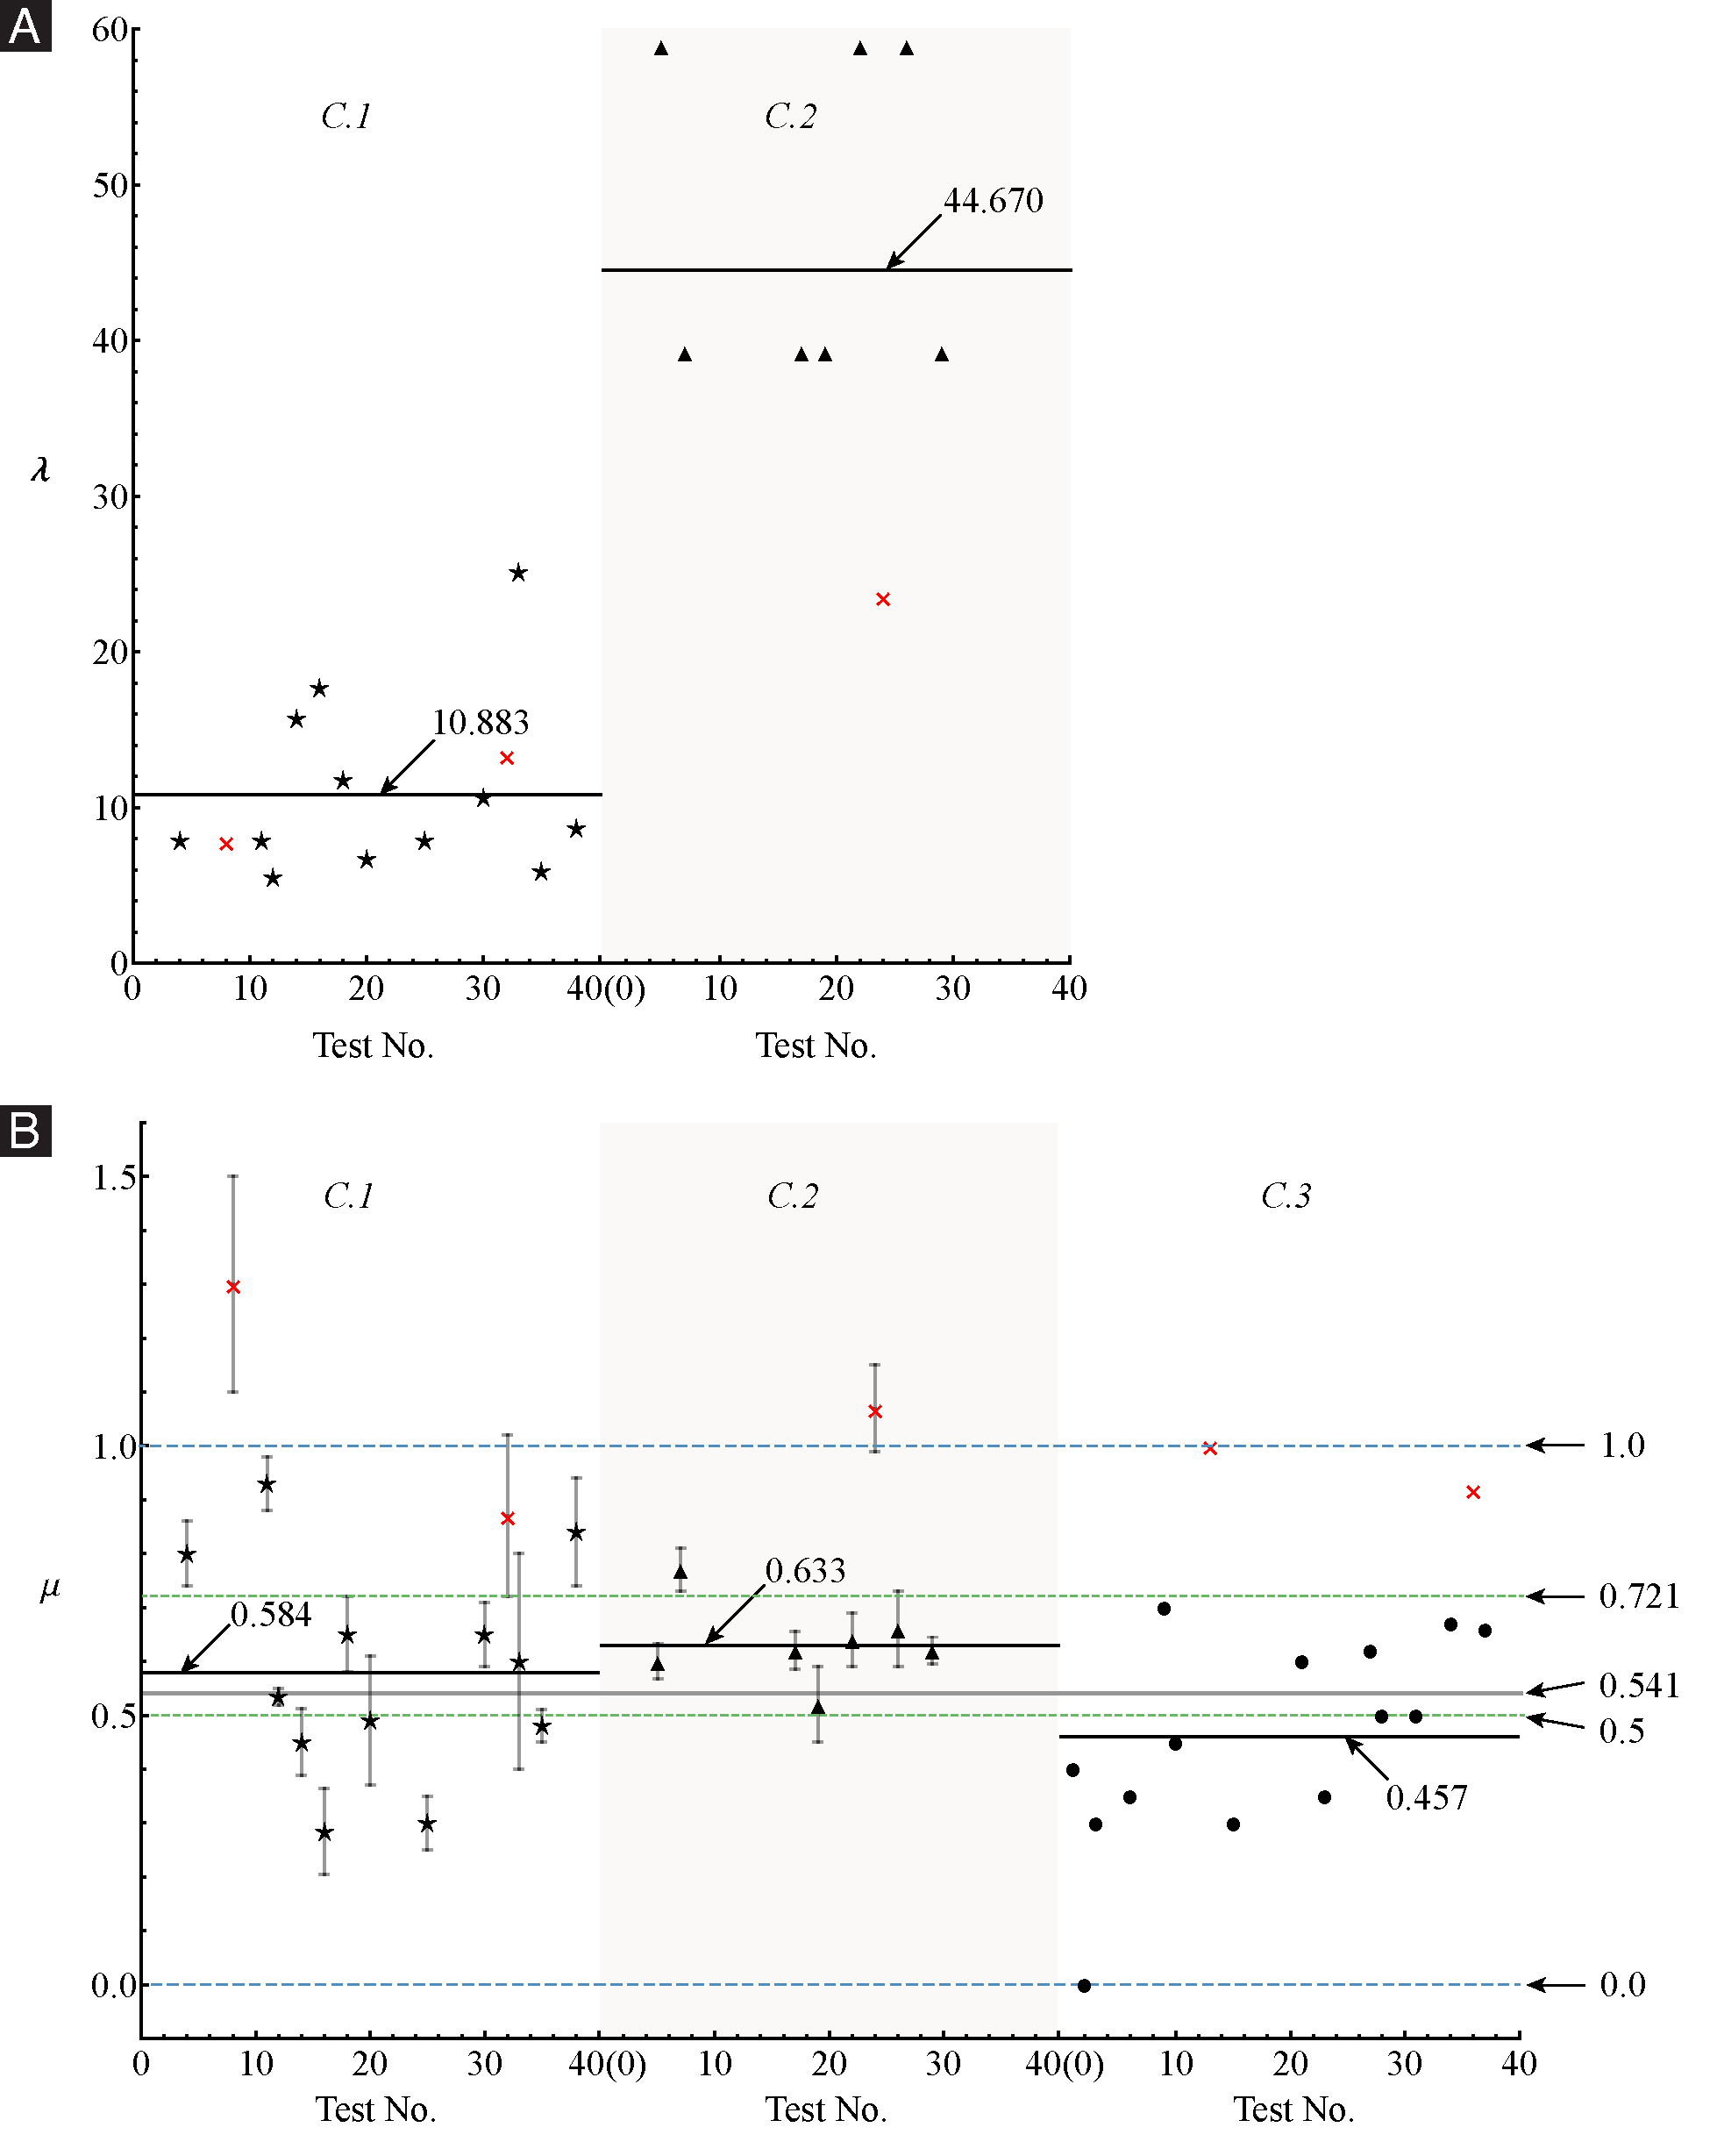
\includegraphics[width=1\textwidth]{../Figures_Submit/Distribution_V2.pdf}
\par\end{centering}
\centering{}
\caption{(Caption continued on next page)}
\label{fig:Distribution}
\end{figure}

\begin{figure}[t]
\centering
\contcaption{Distribution of the values we chose for~$\lambda$
and~$\mu_0$ to get the predictions from our model for the force-displacement curves to compare favorably with their experimental  measurements.
Subfigure $\subf{A}$ consists of two  plots, which show the chosen values for $\lambda$ that we arrived at when comparing to curves from
\textit{C.1} and \textit{C.2}, respectively.
Subfigure $\subf{B}$ consists of three  plots, which show the chosen values for $\mu_0$ that we arrived at when comparing to curves from
\textit{C.1}, \textit{C.2}, and \textit{C.3}, respectively.
All plots belonging to either $\subf{A}$ or $\subf{B}$  share the same $y$-axis.
The $x$-axis in all plots in both $\subf{A}$ and $\subf{B}$ gives the test number, which ranges from 0 to 40.
We use black five-pointed star, black up-pointing triangle, and black
circle to mark the values we chose when comparing, respectively, to curves from~\textit{C.1},~\textit{C.2}, and~\textit{C.3}.
However, if the curve corresponding to a chosen value also  belonged to  \textit{C.4} then we show that chosen value using a red cross.
In each plot a black horizontal line is used to mark the mean of the chosen values in that plot.
In computing the means, we excluded a chosen value if the curve that it  corresponds to also belonged to  \textit{C.4}.
The remainder of the statements in this caption pertain only to $\subf{B}$.
The gray horizontal line (labeled as 0.541) that runs across all plots in $\subf{B}$ marks the mean of values we chose for~$\mu_0$ when
comparing to all curves not from \textit{C.4}.
We  mark the
maximum  (labeled as 0.721) and the minimum  (labeled as 0.5) of the   measured values for the coefficient of friction between glass and steels that are shown in Table \ref{tab:mu0}.
In general, the coefficient of friction is expected to lie between 0 and 1.
These two values are  shown marked using blue dashed lines.
The size of the error bar around each value chosen for $\mu_0$ when comparing to a curve from either \textit{C.1} or \textit{C.2}  is proportional to the value chosen for $A$ in that comparison.
Note that there are no error bars in the plot corresponding to \textit{C.3}, since when comparing to curves from that category we took $A=0$ (see \S\ref{sec:comparison} for details).
}
\end{figure}

\begin{table}[ht!]
\centering
\begin{tabular}{p{0.35\textwidth} p{0.3\textwidth} p{0.24\textwidth} p{0.12\textwidth}}
\toprule
Materials                                        & Geometry      & Surface condition    & Coefficient of friction\\
\midrule
Glass--Hard steel~\cite{Tomlinson1929friction}   & plane--spherical end of a rod (of diameter 2.54mm) & polished, clean, dry & 0.605\\
\addlinespace[0.5em]
Glass--Mild steel~\cite{Tomlinson1929friction}    & plane--spherical end of a rod (of diameter 2.54mm) & polished, clean, dry & 0.721\\
\addlinespace[0.5em]
Glass--Mild steel~\cite{beare1935physical}        & plane--sphere (of diameter 5 mm)  & polished, clean, dry & 0.51-0.61\\
\addlinespace[0.5em]
Glass--Stainless steel~\cite{deulin2010mechanics} & ---          & polished, in vacuum  & 0.5\\
\addlinespace[0.5em]
Stainless steel (with silica coating)--Stainless steel~\cite{marsal2013mechanical} & plane--sphere (of diameter 10 mm) & in air & 0.7\\
\bottomrule
\end{tabular}
\caption{Estimates for the coefficient of friction between glass and steel from literature}
\label{tab:mu0}
\end{table}

\pagebreak{}

\section{Concluding remarks\label{sec:Remark}}
\begin{enumerate}
\item As can be noted from Table~\ref{tab:mu0} and Figure~\ref{fig:Distribution}$\subf{B}$, \sout{
the values chosen for~$\mu_0$, while comparing our model's predictions
to the measurements of~\cite{Sayaka2021Sawtooth},} \textcolor{red}{the values of $\mu_0$, which were chosen to match our model's predictions closely with the measurements of~\cite{Sayaka2021Sawtooth},} are quite
consistent with the values reported in literature for the coefficient
of friction between glass and steel (note that the contact in our
experiments is between silica (spicule) and stainless steel (trench
edge)). This consistency supports the view that it is valid to use
the developed model to interpret Kochiyama et al.'s SS experiments.
\item In order to further gauge the validity of applying the developed model
to interpret the SS experiments, it would be ideal if~$\mu(\cdot)$,
the variation of the coefficient of friction between the spicule and
the trench when different cross-sections of the spicule are in contact
with the trench, could be measured directly and independently of the
SS experiments. In the future, we plan on characterizing~$\mu(\cdot)$
using an Atomic Force Microscope~\cite{kesari2010role,kesari2011effective,deng2019depth}.
Those experiments will provide alternate estimates for~$A$ and~$\lambda$,
which can then be, respectively, compared with the chosen values for
them. That comparison would allow us to further gauge the validity
of applying our model to the SS experiments.
\item It is \sout{quite} unlikely that the friction coefficient varies in a sinusoidal
fashion along the spicule's length. It is even more unlikely\sout{, as we
have assumed in our model,} that the coefficient of friction varies
in the exact same manner at both the left and the right trench edges
during the experiment\textcolor{red}{, as assumed in our model}. The goal of assuming that the variation of
the coefficient of friction along the spicule's length was symmetric
about the spicule's midpoint was \sout{simply }to make the problem tractable.
\sout{The}\textcolor{red}{However, the} decision to model the variation of the coefficient of friction
using a single sinusoid was\sout{, however,} more deliberate. We have compared
the predictions from other versions of our model that incorporate
more realistic variations for the friction coefficient with the experimental
curves. These more realistic variations involved superposition of
multiples sinusoids, and consequently involved a larger number of
free parameters than the presented single sinusoidal variation, which
contains four free parameters, namely~$\mu_0$,~$A$,~$\lambda$,
and~$\phi$. Unsurprisingly, the predictions from those other versions
of our model match the experimental curves better than those from
the presented version of the model. Despite the above fact, we chose
to focus this paper on the version based on the single sinusoidal
variation, since our primary goal was to present insight into the
potential mechanism(s) underlying the sawtooth pattern, rather than
to analytically reproduce the measured curves. And among the different
versions of our model that we studied, we believe that the one based
on the single sinusoidal variation illustrates the sawtooth mechanism
captured by our model in the \sout{most clear}\textcolor{red}{clearest} manner.
\item The mechanism underlying the sawtooth patterns in our experiments
is similar to the surface topography (roughness) based mechanism put
forward for explaining the stick-slip phenomenon~\cite{rabinowicz1966friction,mora1994simulation,berman1996origin}.
The controlling factors in the surface topography mechanism of stick-slip
are the surface's roughness and the stiffness of the loading system,
which are the same as the ones in our model's mechanism for the sawtooth
pattern if we assume that the friction variation in our work is primarily
due to the spicule's surface roughness. One difference in the mechanics
of the SS experiments and the stick-slip phenomenon is that in the
SS experiments, the spicule is slipping both before and after the occurrence
of an instability, while in the stick-slip phenomenon, the specimen
is stationary before the occurrence of an instability, and is sliding
afterwards.
\item Our preliminary research suggests that there can exist a different
model for the SS experiments, which is also capable of capturing the
sawtooth patterns in the measured force-displacement curves. Interestingly,
in that model, it is not required to assume that the coefficient of
friction varies along the spicule's length. Since we were unable to
experimentally ascertain that the coefficient of friction indeed varied
along the spicule's length, a model that does not require the assumption
of a varying friction coefficient may seem preferable to the
one that does. However, \sout{that different}\textcolor{red}{this} model also contains assumptions
that cannot be readily justified through experiments. Furthermore,
we were unable to derive any quantitative predictions from that different
model for the measured force-displacement curves. For these reasons,
we gave preference to the variable friction based model that we presented
in this paper.
\end{enumerate}


\begin{figure}
\centering{}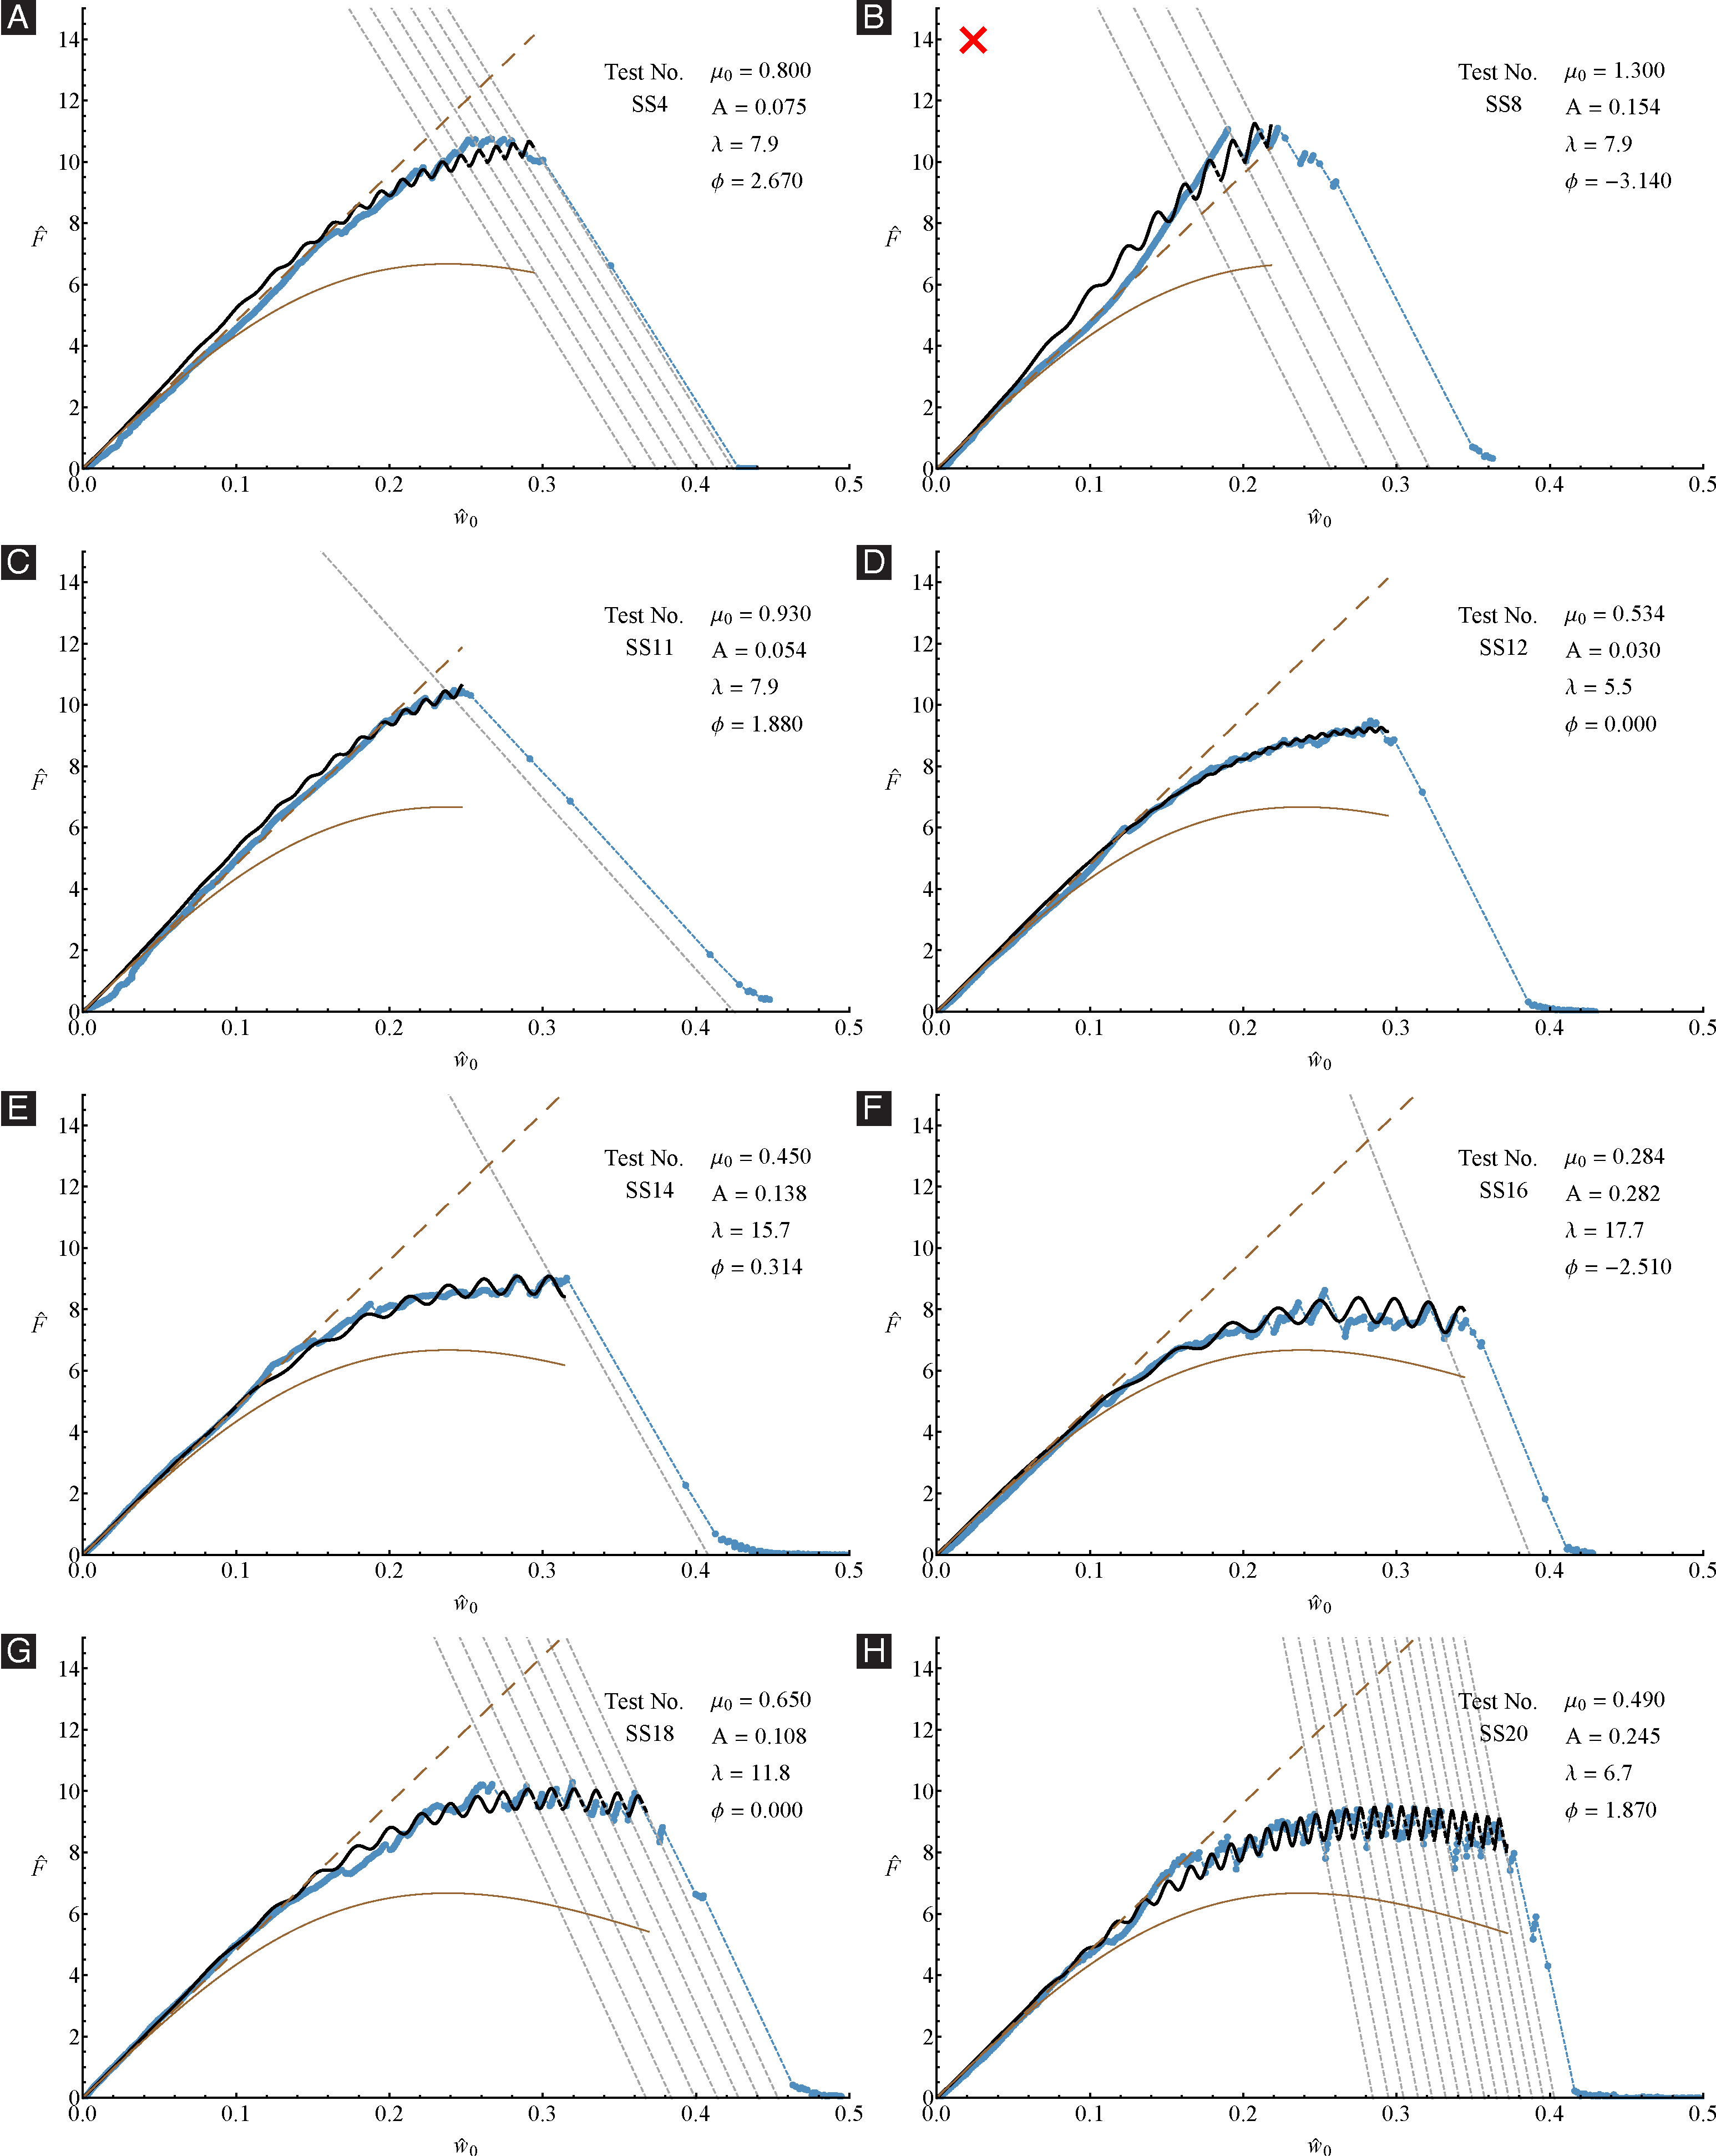
\includegraphics[width=1\textwidth]{../Figures_Submit/Cat1Sub1.pdf}
\end{figure}

\begin{figure}
\begin{centering}
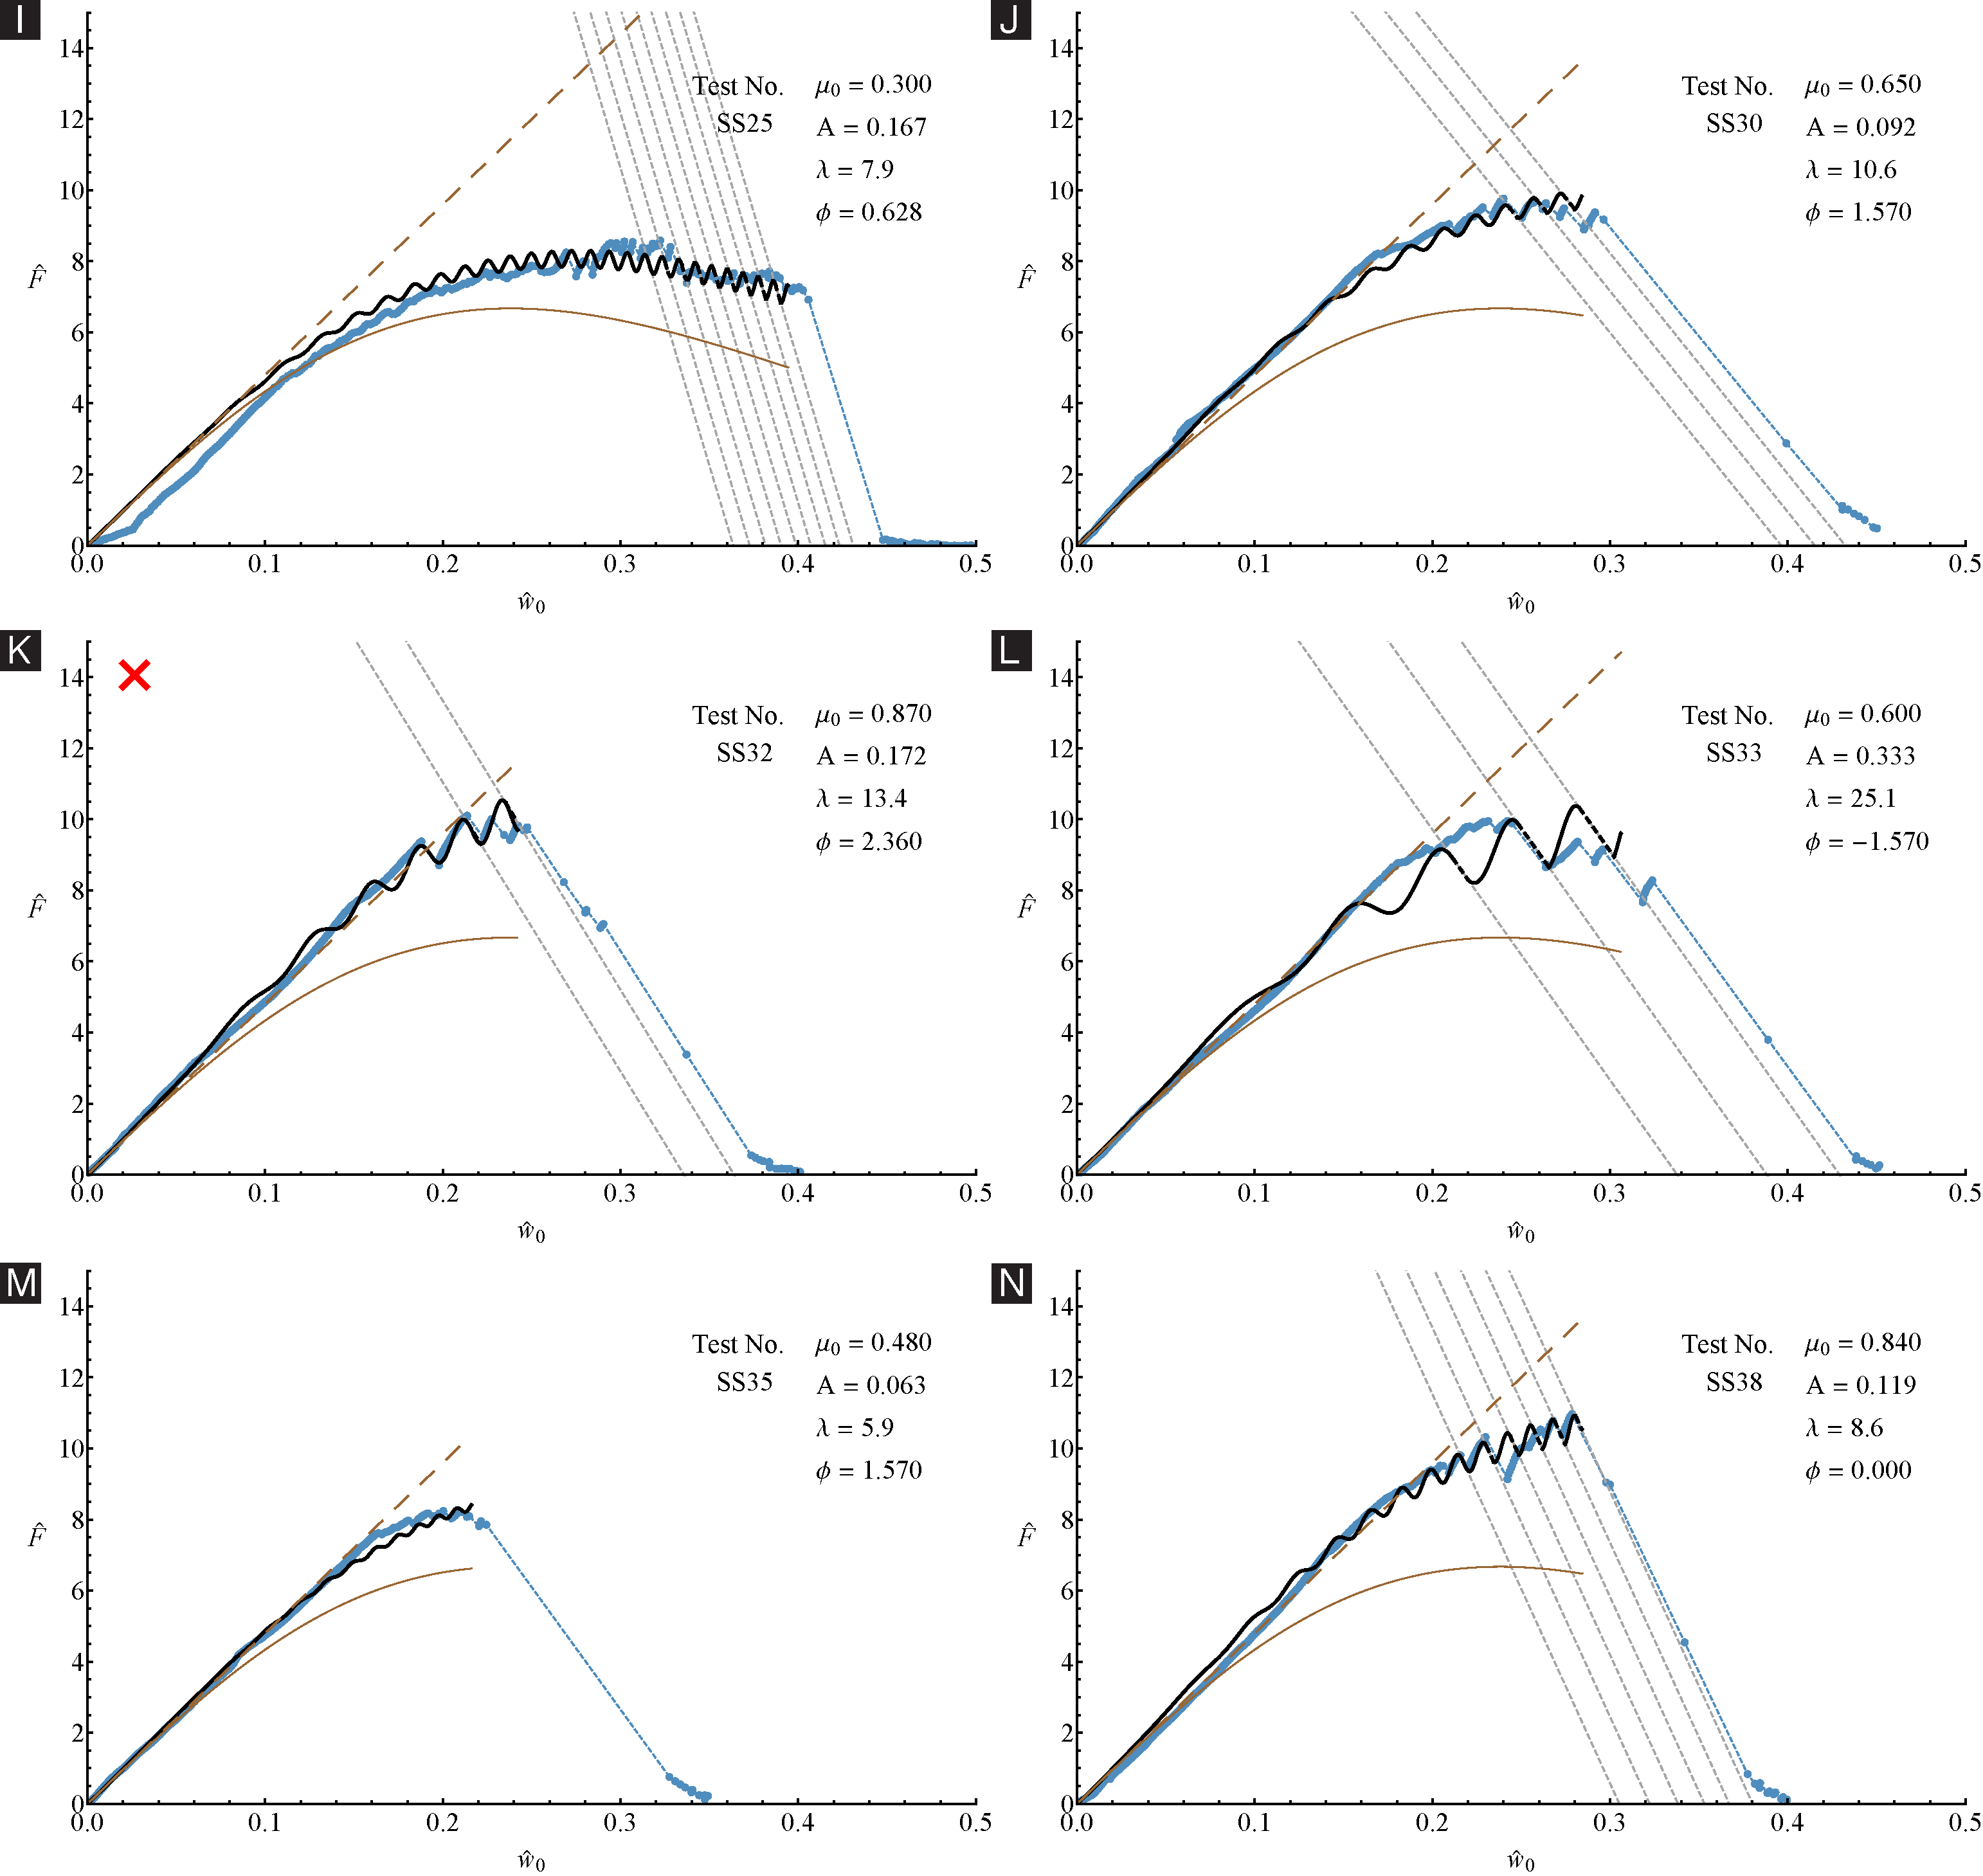
\includegraphics[width=1\textwidth]{../Figures_Submit/Cat1Sub2.pdf}
\par\end{centering}
\caption{
\label{fig:Cat1}
Comparing measured force-displacement curves from the SS tests belonging to category~\textit{C.1} with their theoretical predictions.
Each subfigure corresponds to a different test.
The subfigures with a red cross mark at their top left corners correspond to tests that also belong to category~\textit{C.4}.
The following statements apply to each subfigure separately.
The experimentally measured force-displacement curve is shown in blue.
The prediction from our model for that curve is shown in black.
The values we chose for the parameters~$\mu_0$,~$A$,~$\lambda$, and~$\phi$ in our model for generating that prediction are shown at the top right corner.
The predictions from the Euler-Bernoulli theory and from our model for the case~$\mu_0 = 0$ are shown using brown-dashed and brown-solid lines, respectively.
The gray dashed oblique lines are the graphs of the  function~\eqref{def:Fcant} at the time instances at which we noted a sudden drop in the measured force.
In  generating these graphs, in the function ~\eqref{def:Fcant} we used the $\hat{k}_c$  and $\hat{w}_s(\cdot)$ that we constructed using the experimental details of the  test.
}
\end{figure}

\begin{figure}
\begin{centering}
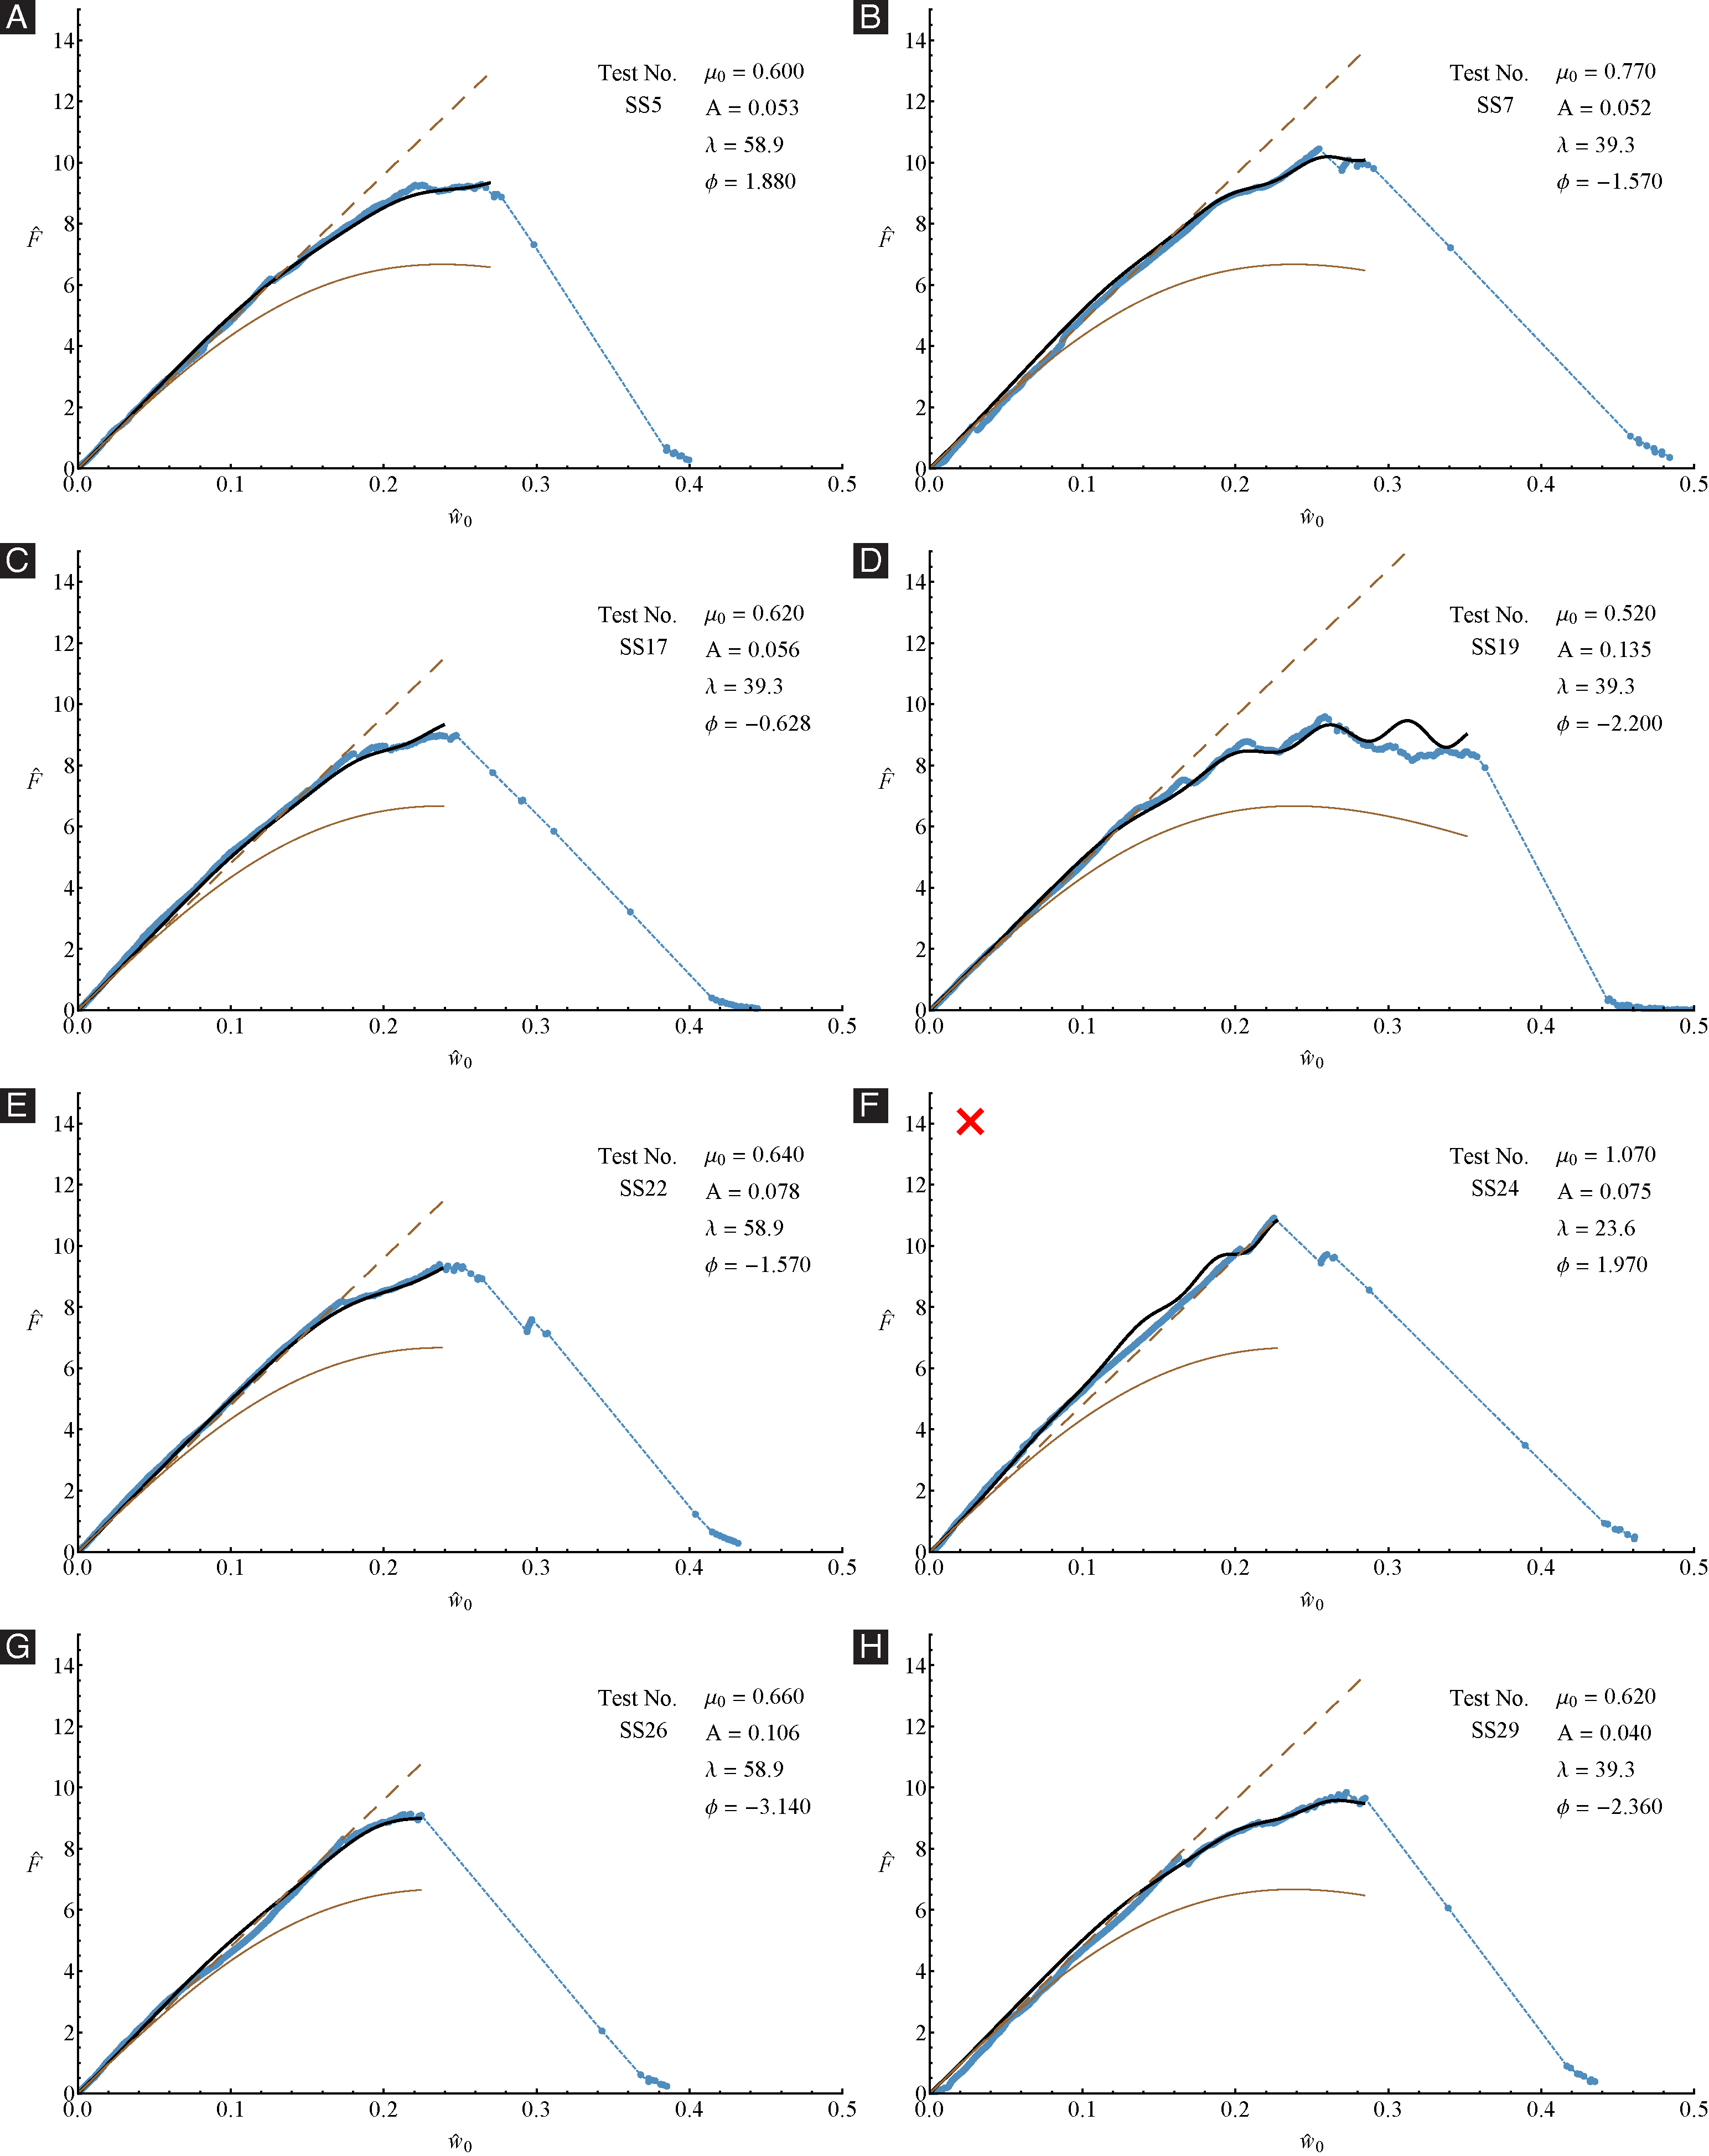
\includegraphics[width=1\textwidth]{../Figures_Submit/Cat2.pdf}
\par\end{centering}
\centering{}
\caption{
\label{fig:Cat2}
Comparing measured force-displacement curves from the SS tests belonging to category~\textit{C.2} with their theoretical predictions.
Each subfigure corresponds to a different test.
The subfigures with a red cross mark at their top left corners correspond to tests that also belong to category~\textit{C.4}.
The statements made in the caption of Figure~\ref{fig:Cat1} that apply  to its subfigures individually apply to the subfigures of this figure individually as well.
}
\end{figure}

\begin{figure}
\centering{}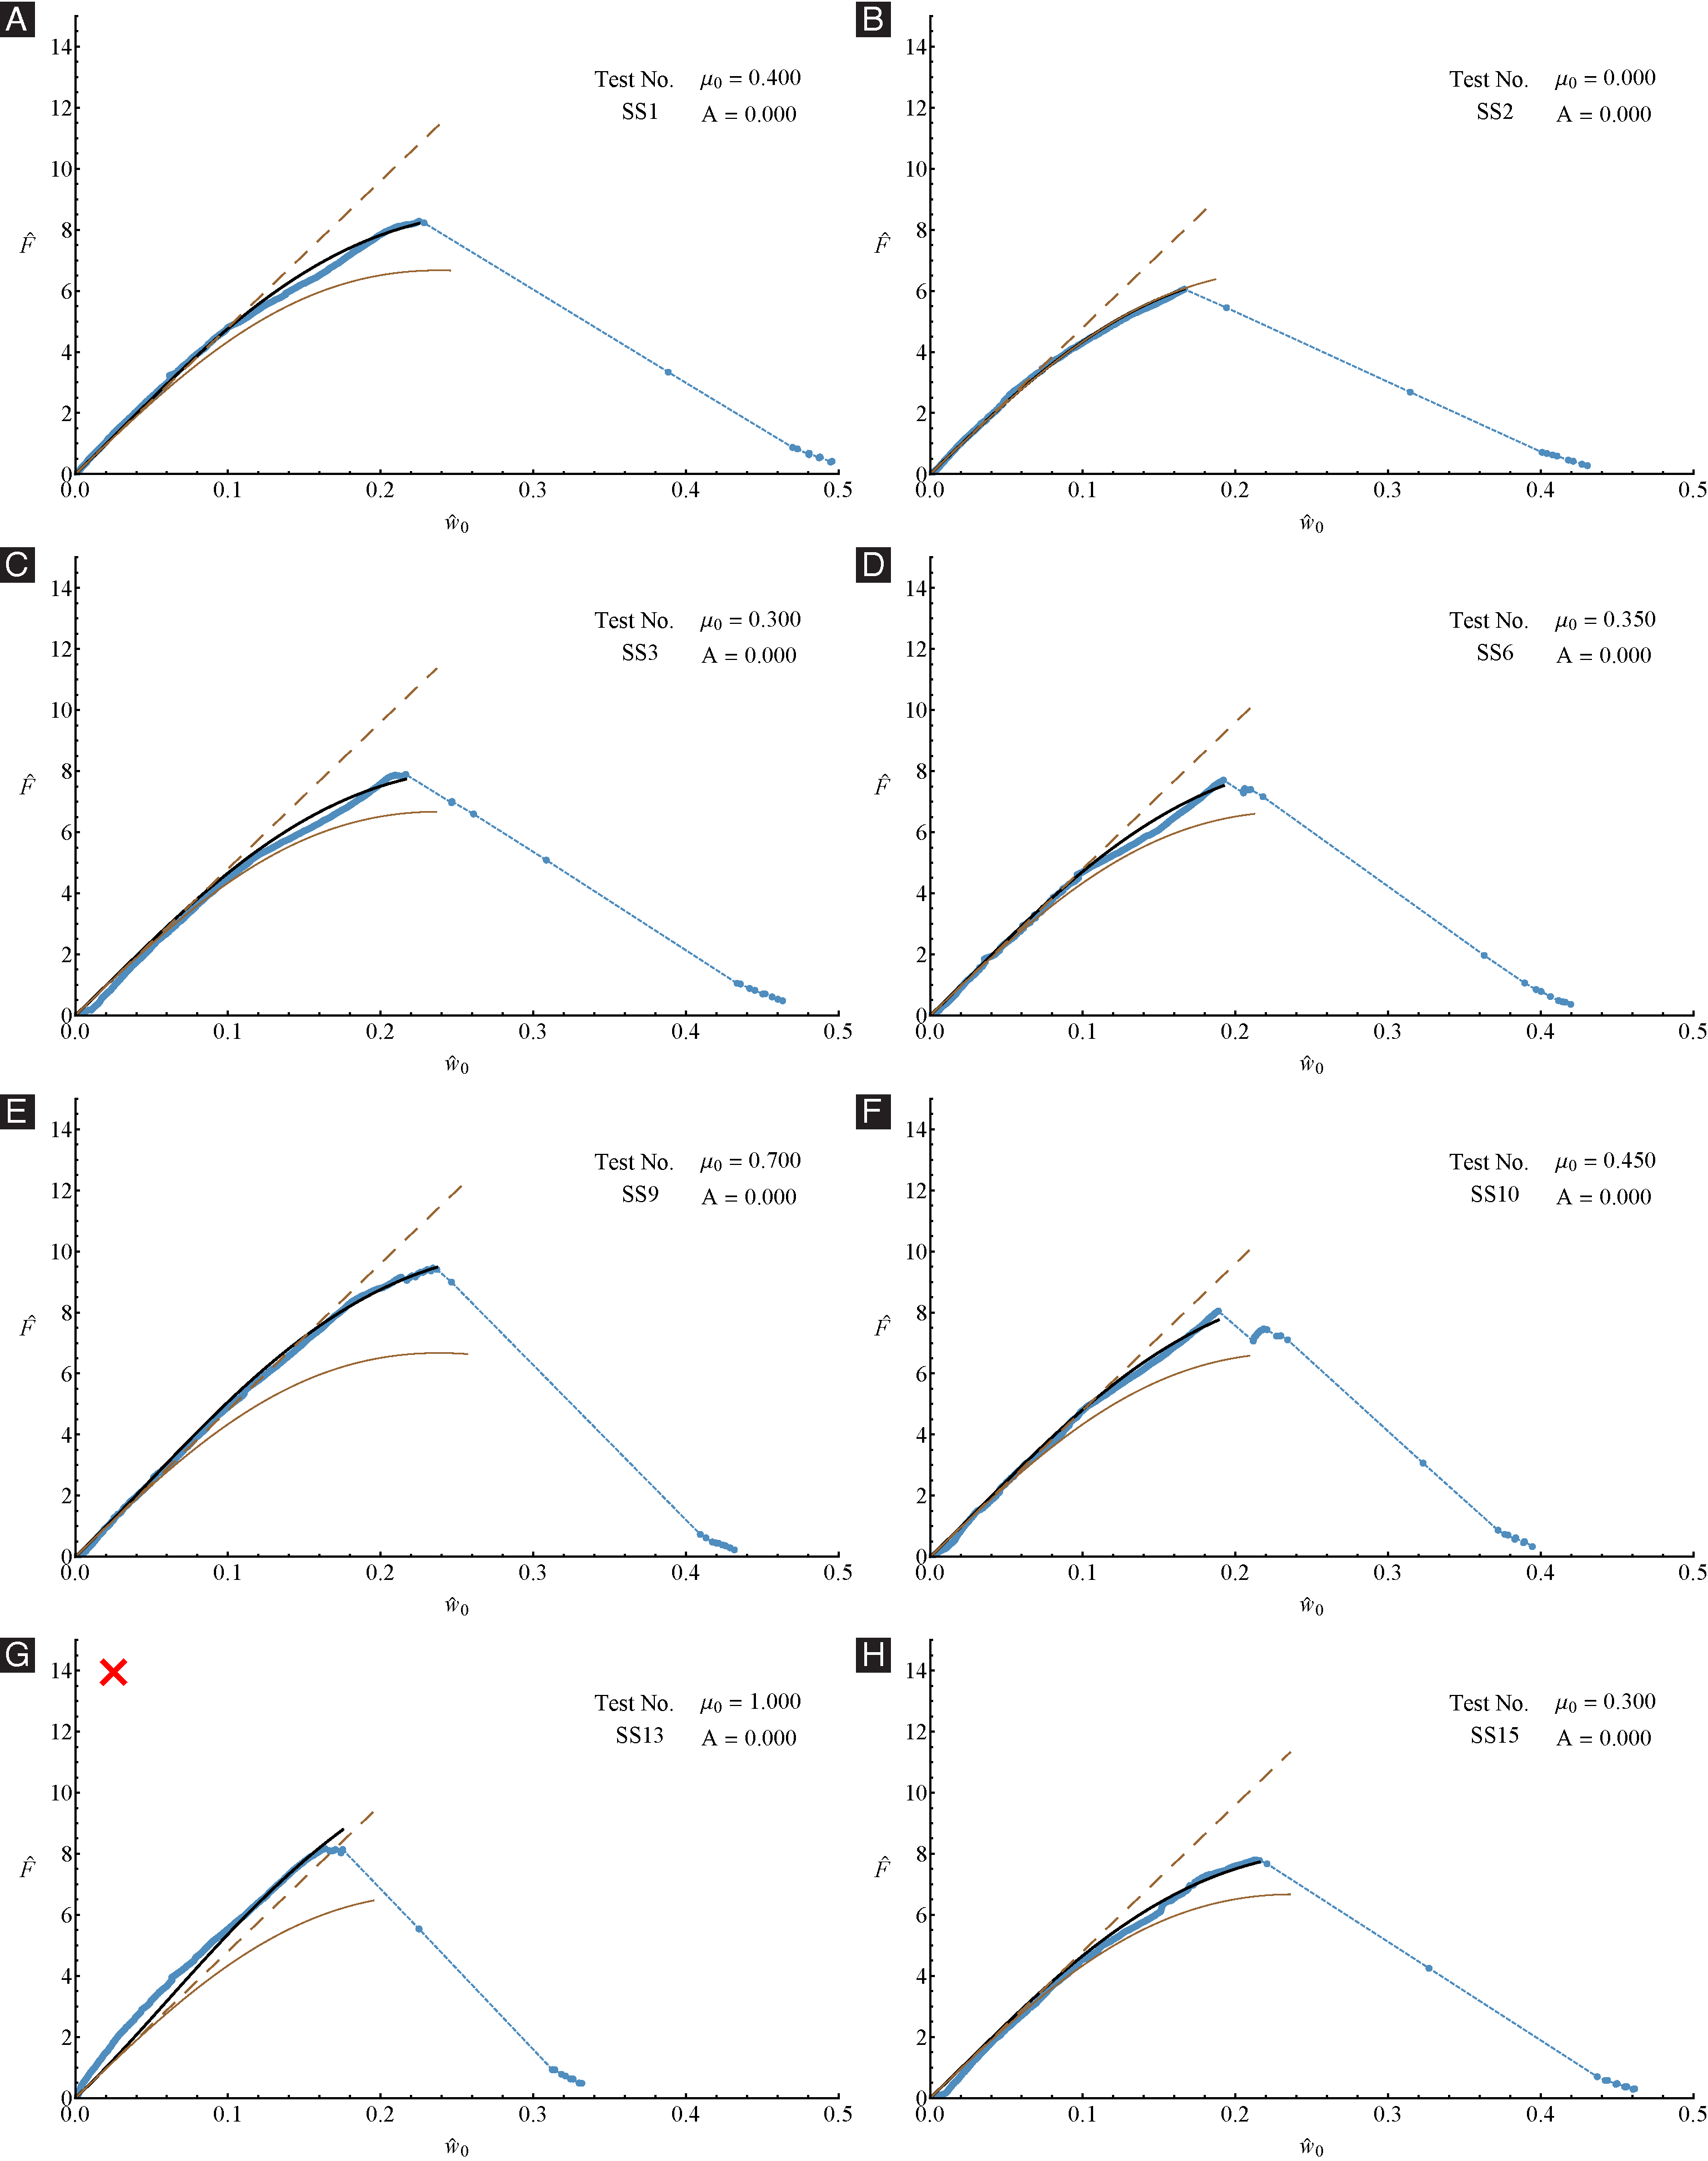
\includegraphics[width=1\textwidth]{../Figures_Submit/Cat3Sub1.pdf}
\end{figure}

\begin{figure}
\begin{centering}
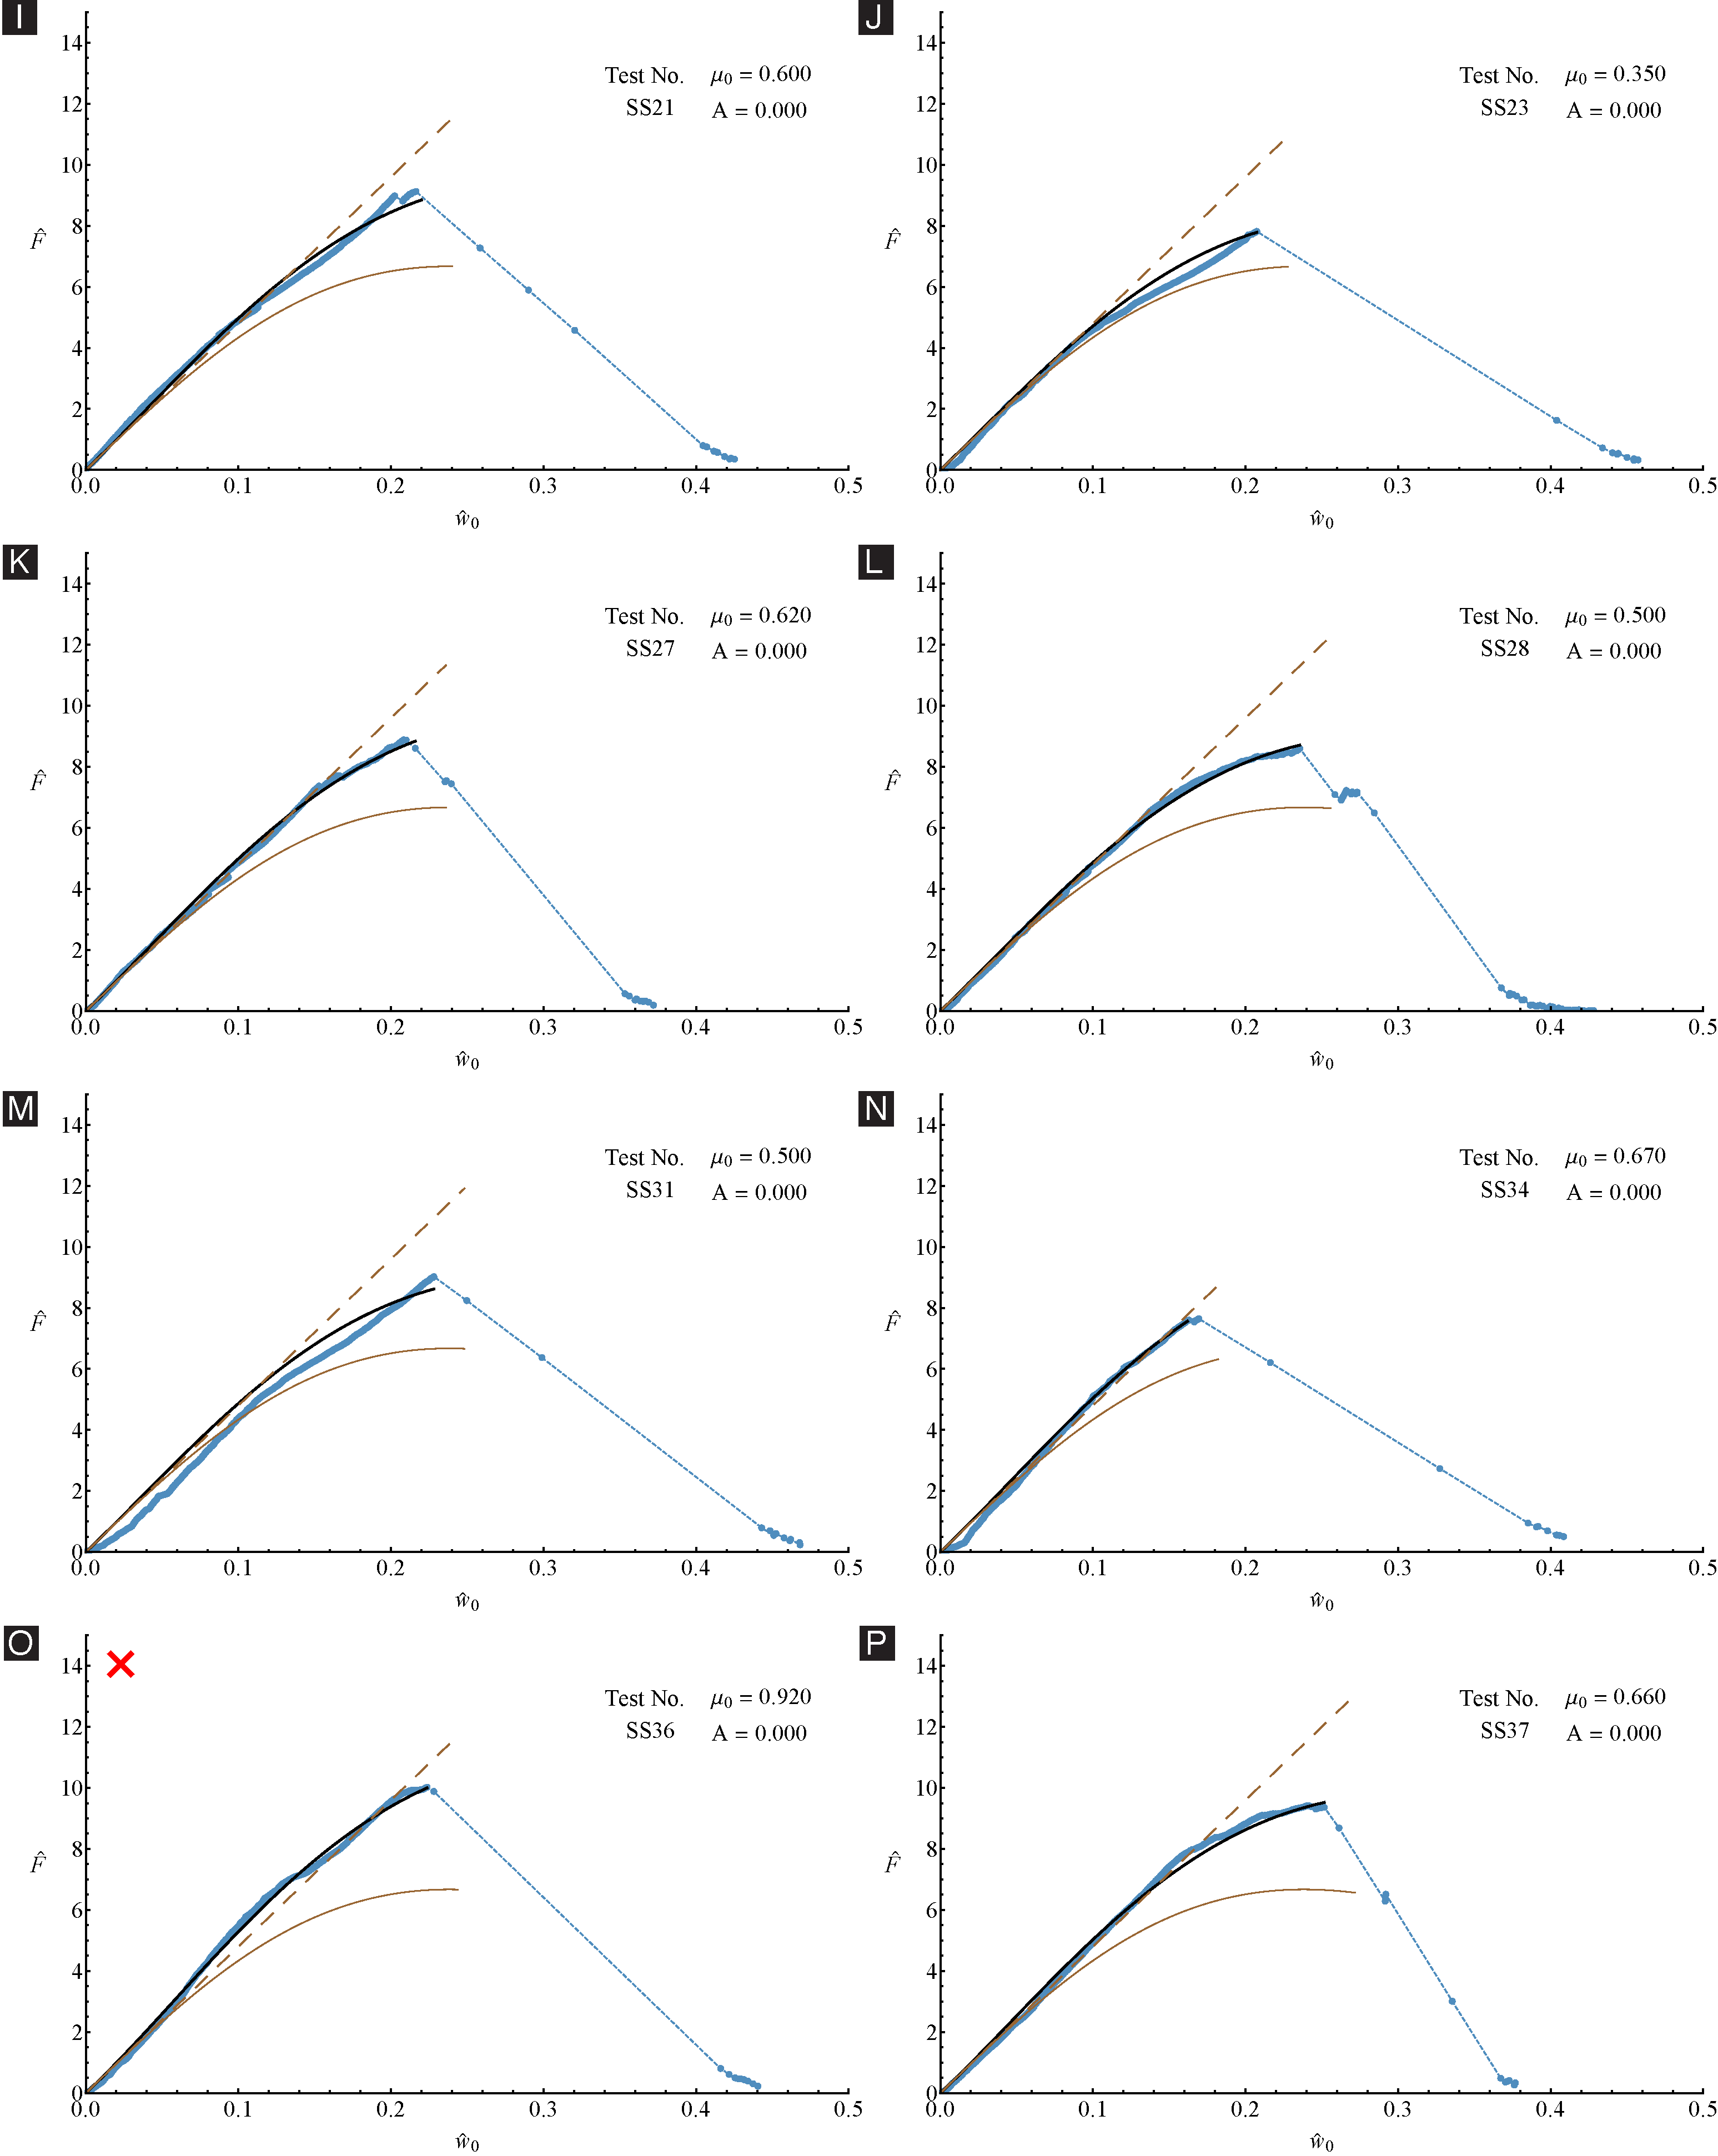
\includegraphics[width=1\textwidth]{../Figures_Submit/Cat3Sub2.pdf}
\par\end{centering}
\caption{\label{fig:Cat3}Comparing measured force-displacement curves from the SS tests belonging to category~\textit{C.3} with their theoretical predictions.
Each subfigure corresponds to a different test.
The subfigures with a red cross mark at their top left corners correspond to tests that also belong to category~\textit{C.4}.
The statements made in the caption of Figure~\ref{fig:Cat1} that apply  to its subfigures individually apply to the subfigures of this figure individually as well.}
\end{figure}

\begin{figure}
\begin{centering}
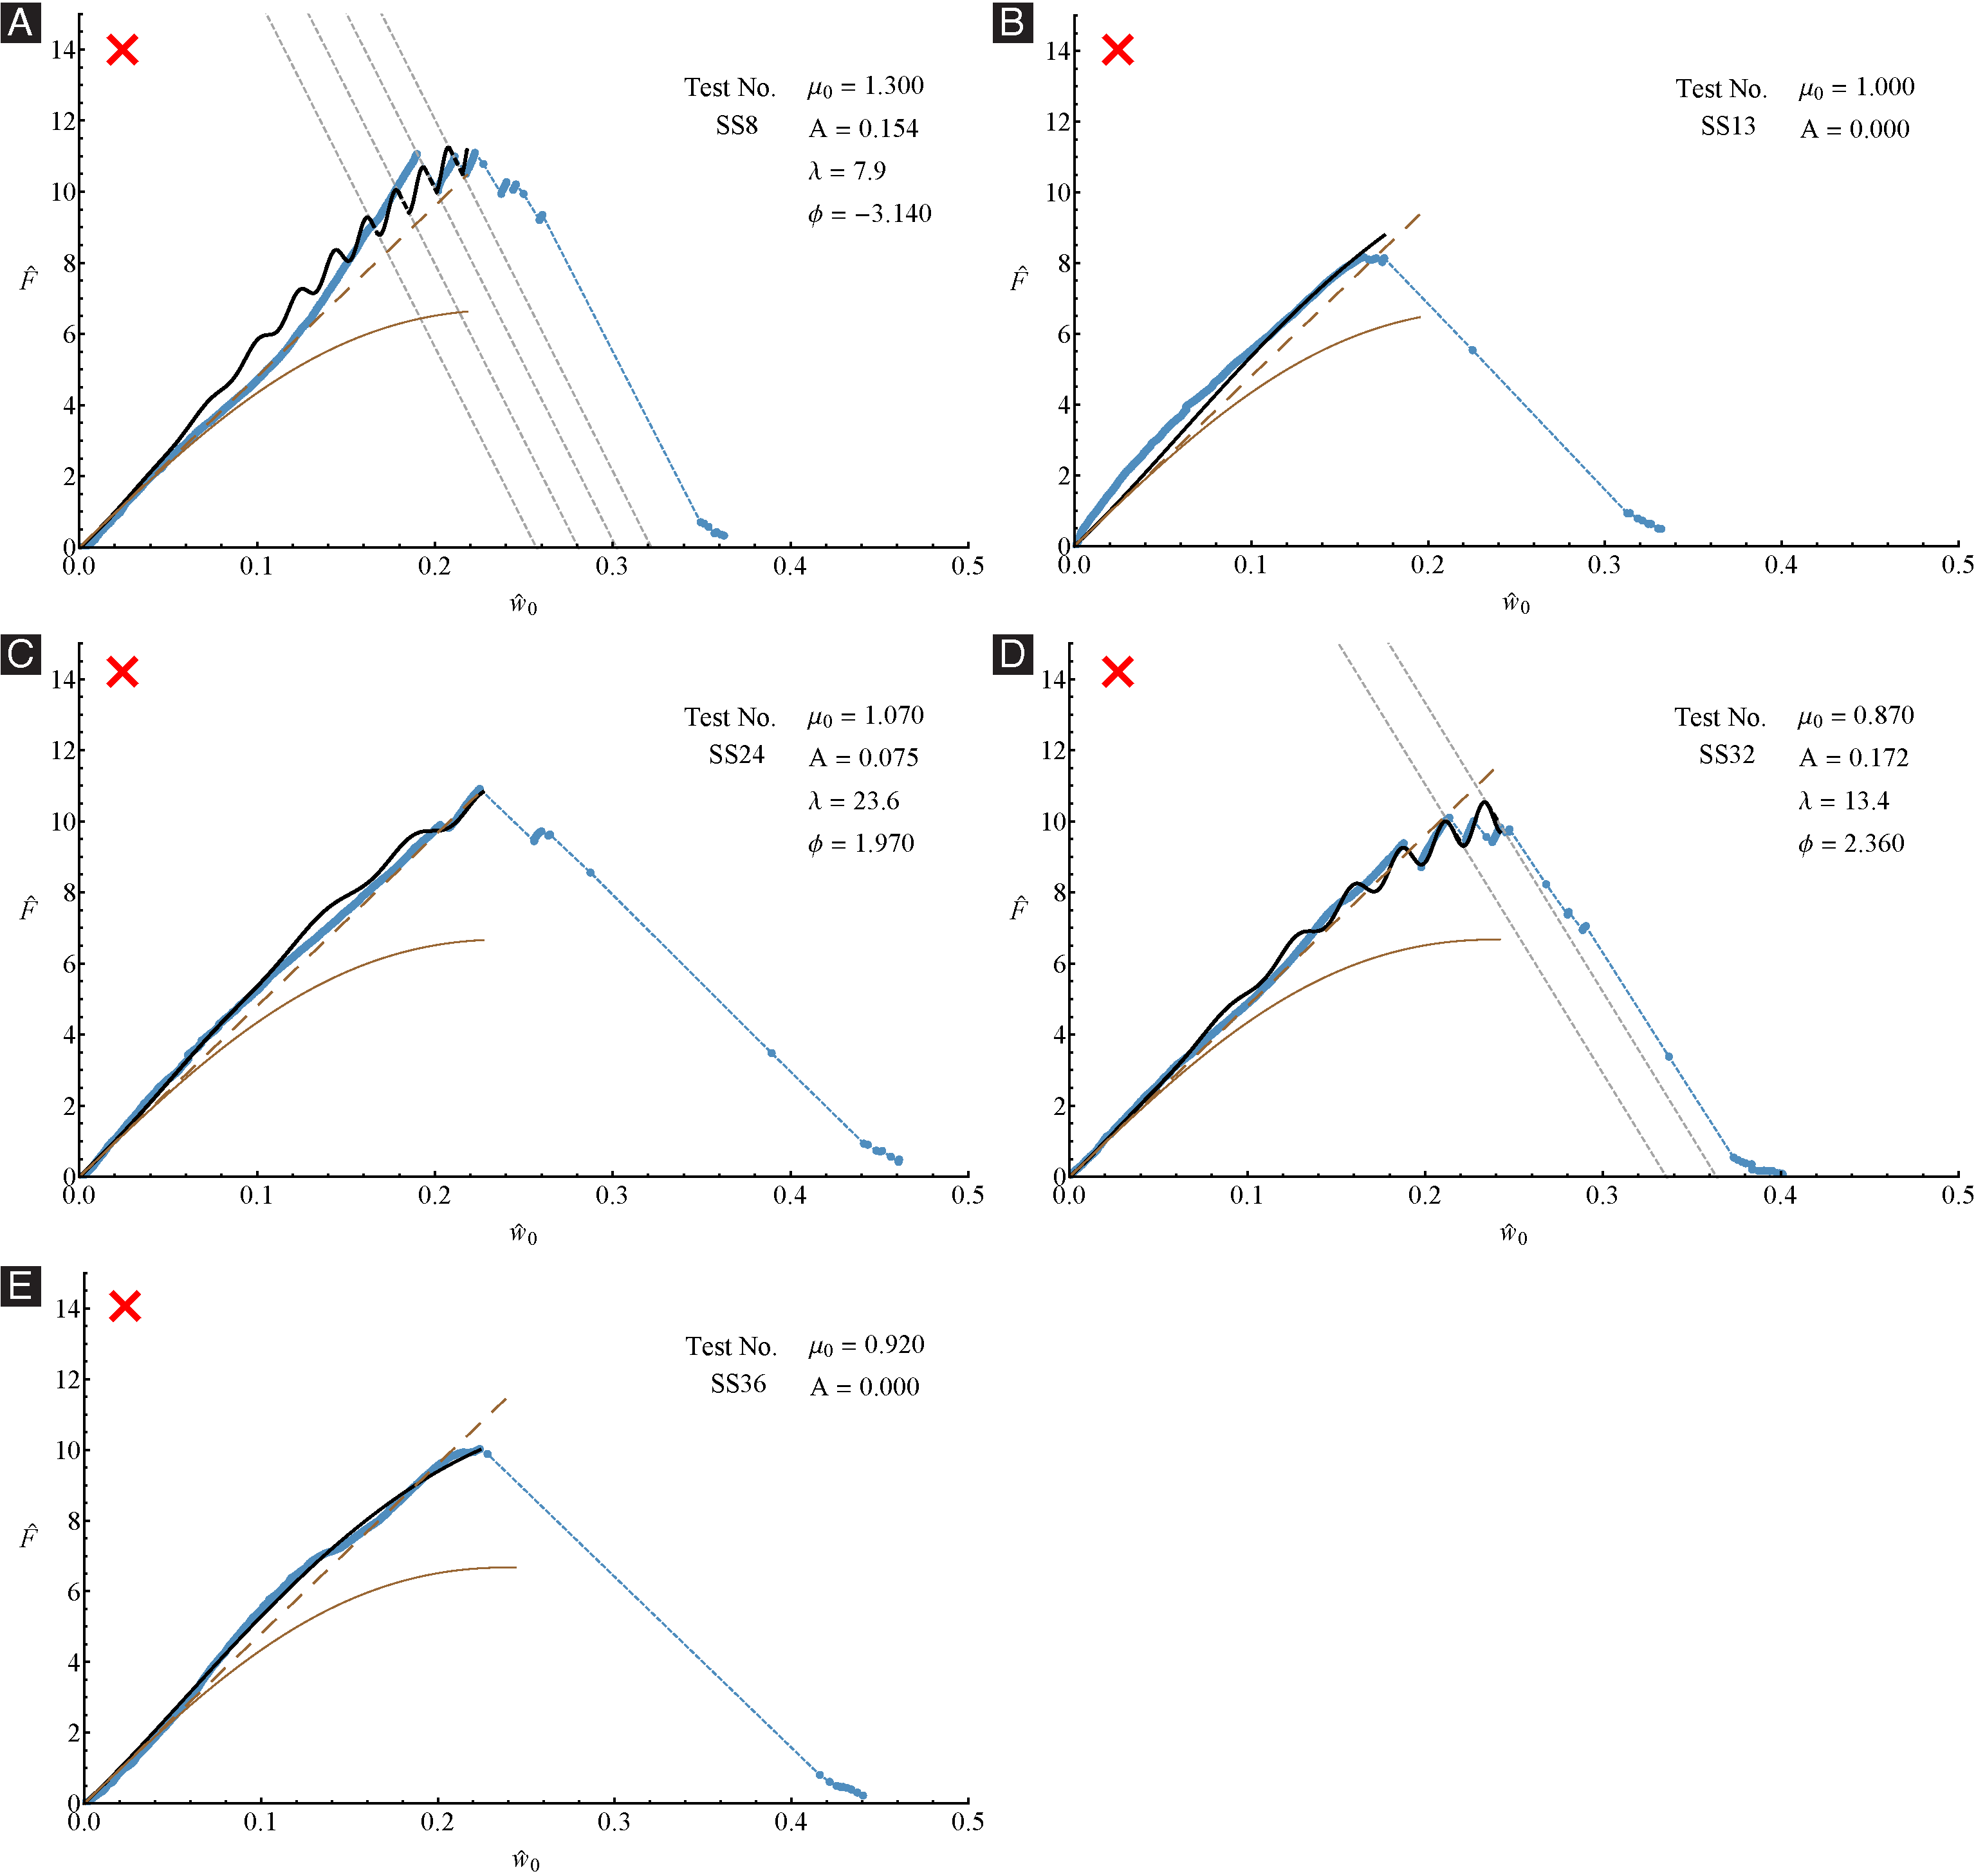
\includegraphics[width=1\textwidth]{../Figures_Submit/Cat4.pdf}
\par\end{centering}
\centering{}\caption{\label{fig:Cat4}Comparing measured force-displacement curves from the SS tests belonging to category~\textit{C.4} with their theoretical predictions.
Each subfigure corresponds to a different test.
The statements made in the caption of Figure~\ref{fig:Cat1} that apply  to its subfigures individually apply to the subfigures of this figure individually as well.}
\end{figure}


\newpage

\bibliographystyle{elsarticle-num}
\bibliography{../refm_V2}


\end{document}

lks;lask;lskd;lk%%
%% End of file `elsarticle-template-num.tex'.
$this $
Note that the chosen~$A$ value is non-zero when comparing to the curves
from~\textit{C.1} and~\textit{C.2}, while~$A$ vanishes when
comparing to the curves from~\textit{C.3}.
